\documentclass[11pt]{article}

% Change "review" to "final" to generate the final version.
% Change to "preprint" to generate a non-anonymous version with page numbers.
\usepackage[review]{acl}

\usepackage{times}
\usepackage{latexsym}
\usepackage{booktabs}
\usepackage{longtable}
\usepackage{makecell}
\usepackage{multirow}
\usepackage{amssymb}
\usepackage{amsmath}
\usepackage{xcolor}
\usepackage{subcaption}
\usepackage[T1]{fontenc}
\usepackage[utf8]{inputenc}
\usepackage{microtype}
\usepackage{inconsolata}
\usepackage{graphicx}
\graphicspath{{figures/}}

% Float packing. ACL's defaults leave large slack around the six full-width
% floats in the main text; these values keep the layout legible while removing
% the unused vertical space that pushed numbered content onto a ninth page.
\setlength{\textfloatsep}{12pt plus 2pt minus 2pt}
\setlength{\dbltextfloatsep}{12pt plus 2pt minus 2pt}
\setlength{\floatsep}{10pt plus 2pt minus 2pt}
\setlength{\dblfloatsep}{10pt plus 2pt minus 2pt}
\setlength{\intextsep}{10pt plus 2pt minus 2pt}
\captionsetup{skip=4pt}
\renewcommand{\topfraction}{0.9}
\renewcommand{\dbltopfraction}{0.85}
\renewcommand{\bottomfraction}{0.5}
\renewcommand{\floatpagefraction}{0.8}
\renewcommand{\dblfloatpagefraction}{0.8}
\renewcommand{\textfraction}{0.1}

\title{Semantic Matching in Medieval Latin: A Benchmark, Layerwise Analysis, and Geometric Repair}

\author{First Author \\
  Affiliation / Address line 1 \\
  Affiliation / Address line 2 \\
  Affiliation / Address line 3 \\
  \texttt{email@domain} \\\And
  Second Author \\
  Affiliation / Address line 1 \\
  Affiliation / Address line 2 \\
  Affiliation / Address line 3 \\
  \texttt{email@domain} \\}

\begin{document}
\maketitle

\begin{abstract}
Medieval canon law before the twelfth century survives in many compilations, whose manuscripts differ in spelling and in the selection and arrangement of their elements. We introduce a Medieval Latin benchmark of 840 labelled canon-law fragments with 1,705 manuscript witnesses, and we define two tasks on it: pairwise duplicate detection and open-set directory routing. Our question is where inside a pre-trained encoder the retrieval signal lives, why it disappears, and what recovers it. A layerwise analysis of six pre-trained models from three architectures separates two effects that are easy to conflate. Anisotropy is universal across the six models: every model has a layer where the mean cosine between randomly selected passages reaches 0.23 to 0.95, and no baseline layer in any model separates equivalent from non-equivalent passages by more than 0.29 in mean cosine. Catastrophic mid-depth collapse is not universal: the Latin and multilingual T5 encoders fall to AUROC 0.496, 0.538, and 0.654 in their middle layers, while LaBSE, Qwen3-0.6B, and KaLM-mini improve close to monotonically with depth. All-but-the-Top post-processing, fit only on training embeddings, repairs all six. Best-layer AUROC moves into a 0.971 to 0.987 band, the cosine gap rises to between 0.525 and 0.611, and the spread in directory accuracy at rank 1 across models falls from 39.3 points to 3.3. Under the repair, integrated gradients and retrieval-adapted MaRC give a narrow answer: ABTT improves leave-one-out rank faithfulness in five of six LaTa, PhilTa, and mT5-base model-method cells, the sixth a tie, while ERASER-style rationale metrics show mixed effects.
\end{abstract}

\section{Introduction}

\begin{figure*}[!t]
\centering
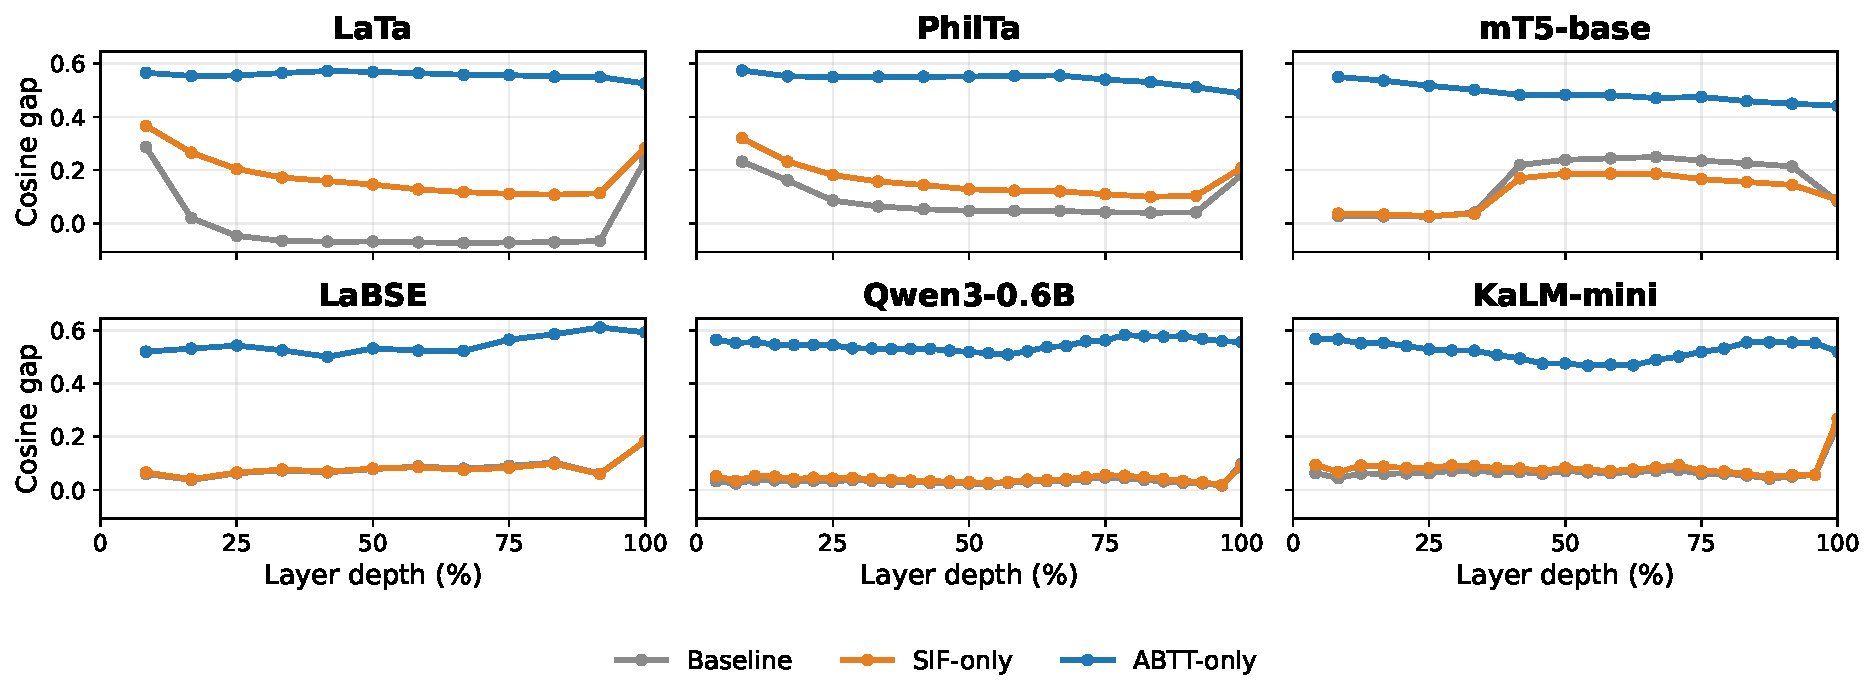
\includegraphics[width=0.96\textwidth]{fig_release_gap_6model.pdf}
\caption{Cosine gap against layer depth for all six models: mean cosine of same-directory pairs minus mean cosine of different-directory pairs, the margin a threshold works with, so larger is better. Gray is baseline mean pooling, blue is ABTT-only with $D$ tuned on train, orange is SIF-only. Baseline stays under 0.29 at every layer of every model, and under 0.11 for Qwen3-0.6B. Mid-depth in the top row, the LaTa and PhilTa baseline gap collapses toward zero with their retrieval; the mT5-base gap rises as its ranking fails, which only AUROC (Figure~\ref{fig:dip}) shows. ABTT lifts all six near 0.5 at every depth. SIF-only helps LaTa and PhilTa and leaves the other four near baseline.}
\label{fig:gap}
\end{figure*}

Medieval canon law preserves early records of legislation and judicial opinions in Western Europe. Before the twelfth century it survives not as one stable text but in many compilations, whose manuscripts differ in spelling, wording, fragment boundaries, and transmission history. Deciding whether two passages express the same legal content despite those surface changes drives editorial work: identifying duplicates, analyzing witnesses, and tracing how a text was transmitted.

We study this problem as semantic matching on a benchmark of 840 labelled fragments of Medieval Latin canon law, each a canon or excerpt with one or more manuscript witnesses, 1,705 in all. Task A asks whether two passages express the same meaning. Task B turns the same embeddings into an open-set workflow: route a new passage to an existing directory, or mark it as new. Our question is where inside a pre-trained encoder the retrieval signal lives, why it disappears, and what recovers it.

A final-layer vector cannot answer that, so we work layer by layer, and the layerwise view of six models separates two effects that are often reported together. Anisotropy is universal on this corpus: every model has a layer where pooled passages crowd into a narrow cone, with mean cosine between randomly selected passages reaching 0.23 to 0.95, and no baseline layer of any model separates equivalent from non-equivalent passages by more than 0.29 in mean cosine (Figure~\ref{fig:gap}). A catastrophic mid-depth collapse of retrieval is not universal. LaTa and PhilTa fall to chance in their middle layers and mT5-base loses more than half of its above-chance separation, while LaBSE, Qwen3-0.6B, and KaLM-mini improve close to monotonically with depth.

Anisotropy motivates our use of All-but-the-Top (ABTT) post-processing \citep{mu2018allbutthetop}. We apply it after pooling with no update to model parameters: fit the dominant principal components on training embeddings, remove them from train and test embeddings, then score by cosine. The repair, unlike the collapse, is universal: ABTT lifts every model into a narrow high-accuracy band on both tasks, and at each T5 encoder's worst baseline layer it recovers pairwise AUROC to within 1.0 point of that model's best ABTT layer. SIF weighting \citep{arora2017sif}, which reweights tokens by frequency before pooling, corrects part of the same direction but helps only the collapsed models, and SIF-only never matches ABTT-only.

Geometry diagnoses collapse and recovery but does not select the retrieval layer: a train-only rule (Section~\ref{sec:layers}) locks LaTa layer 7, PhilTa layer 1, and mT5-base layer 1 before any attribution metric is computed.

Finally, we compare local explanations of the score before and after the repair. Integrated gradients \citep{sundararajan2017axiomatic} gives a gradient view of token importance and retrieval-adapted MaRC \citep{brinnerzarriess2023marc} a learned-mask view, with MaRC's classification target replaced by the pairwise retrieval cosine; both explain a fixed query-candidate score and stay local diagnostics.

This paper makes four contributions:
(1) we introduce a benchmark for semantic matching in Medieval Latin canon law, together with a routing task that states the scholar's decision directly: file an unidentified witness under a known fragment, or flag it as new;
(2) we separate, across six models, universal anisotropy from the mid-depth retrieval collapse that only the three T5 encoders show, measuring both with top-PC dominance, effective rank, and cosine concentration;
(3) we show that ABTT repairs the anisotropy on this corpus without updating parameters, compressing a 39.3-point spread in directory accuracy at rank 1 to 3.3 points, with the largest gains on the T5 encoders; and
(4) we adapt token attribution to bi-encoder retrieval, comparing a MaRC-style learned mask with integrated gradients at predeclared retrieval-selected layers; on present evidence ABTT improves leave-one-out rank faithfulness in five of six model-view cells, the sixth a tie, while ERASER-style rationale metrics stay mixed.

\section{Related Work}
\label{sec:related}

\paragraph{Anisotropy, layer geometry, and repair.}
Pre-trained embedding spaces occupy narrow cones \citep{gao2019degeneration, ethayarajh2019contextual, godey2024anisotropy}, where a few coordinates dominate cosine similarity \citep{kovaleva2021bertbusters, timkey2021rogue}. Post-hoc corrections remove or rescale those directions \citep{mu2018allbutthetop, su2021whitening} or downweight frequent tokens before pooling \citep{arora2017sif}. Probing finds information spread across depth \citep{tenney2019pipeline, liu2019linguistic}, and intermediate layers can beat the last \citep{skean2025layer}. Multilingual analyses are rarer \citep{rajaee2022mbert}. We reuse ABTT unchanged on low-resource retrieval, using geometry to measure anisotropy and a train-only rule to pick layers.

\paragraph{Latin and classical-language NLP.}
Latin has dedicated encoders and encoder-decoders \citep{bamman2020latinbert, riemenschneider2023lata}, and appears in multilingual sentence encoders \citep{feng2022labse}, mT5 \citep{xue2021mt5}, and decoder-only LLM embedders \citep{qwen3embedding2025, kalm2025embedding}. Shared tasks target tagging \citep{sprugnoli2020evalatin}, retrieval work focuses on allusion \citep{riemenschneider2023sphilberta}, and work on charters looks at semantic change \citep{liu2024medieval}. No general embedding benchmark \citep{thakur2021beir, muennighoff2023mteb} covers medieval Latin retrieval.

\paragraph{Text reuse in digital humanities.}
Text-reuse systems match n-grams \citep{coffee2012tesserae}, align reprinted newspapers \citep{smith2013infectious}, and add distributional semantics for allusive reuse \citep{manjavacas2019allusive, burns2021intertextuality}, ranking candidates in a closed collection. Our routing task is open-set: a witness may match no labelled fragment in the collection.

\paragraph{Faithfulness of token attributions.}
Integrated gradients \citep{sundararajan2017axiomatic} and learned input masks \citep{brinnerzarriess2023marc} attribute a score to tokens, and much work asks whether attributions are faithful \citep{jain2019attention, jacovi2020faithfully}. Erasure and perturbation protocols \citep{deyoung2020eraser, atanasova2020diagnostic} target classification; retrieval explanation targets ranking \citep{anand2022xir}. We apply them to a bi-encoder cosine score and report where faithfulness improves and where it does not.


\section{Task and Dataset}

\subsection{Task Definition}
\label{sec:tasks}

The benchmark defines two tasks over the same witnesses and the same pooled embeddings. They differ in what the system has to decide.

\paragraph{Task A: pairwise duplicate detection.}
Let $p_1$ and $p_2$ be two passages and let $\equiv$ denote semantic equivalence. The label is $y=1$ if $p_1 \equiv p_2$ and $y=0$ otherwise. The model scores the pair by $\cos(e_{p_1}, e_{p_2})$ over pooled embeddings. Task A uses no directory structure and no threshold at scoring time, and evaluation uses the test $n \times n$ cosine matrix.

\paragraph{Task B: directory routing.}
Task B uses the same embeddings in a scholar-facing retrieval workflow: given a query passage $q$ and the existing labelled directories, the system routes $q$ to a directory or marks $q$ as new. In autonomous routing, a threshold $\tau$ fit on training same-directory and different-directory pairs decides whether the query enters its nearest neighbour's directory or the new class; in top-$k$ ranking, each directory receives its best document match score, a pseudo-option \texttt{\_\_NEW\_\_} receives score $\tau$, and the simulated expert succeeds when the labelled directory appears in the shortlist.

\subsection{Dataset Construction}

The corpus contains 1,705 Medieval Latin canon-law witnesses (manuscript copies of a text, each identified by its siglum: Place-Library-Shelfmark) from the Carolingian Canon Law project \citep[CCL;][]{firey2009ccl, eichbauer2014ccl}, an open-access digital edition founded in 2009.\footnote{Founding year, pre-2019 workflow, proofreading standard and the one HTR-transcribed manuscript: project director, personal communication, 2026.} Most manuscripts are ninth-century and unedited to modern standards. Transcription is manual, from manuscript images or, for some texts, eighteenth-century printings, with one exception: handwritten text recognition has been attempted on one manuscript (Paris, BnF, lat.\ 1454; 142 of the 1,705 witnesses), and its transcription is still in proofreading. Before 2019 transcribers worked from microfilm and CCL contributors converted the files to TEI-P5 (the Text Encoding Initiative's XML standard for scholarly editions). Since 2019 they transcribe in the CCL Transcription Desk beside a IIIF image of the folio (a zoomable web-served scan of the manuscript leaf); an approved proofreader then checks it against the image to the letter and adds TEI markup \citep{ccl2026desks}. The interface credits the transcriber and proofreader of each unit (one transcribed canon or excerpt) \citep{ccl2026about}. We hold the witnesses as plain text derived from the CCL TEI-P5 export, with the labels as supplied.

CCL keys every unit to its original source, such as a fourth-century council or a papal decretal, and our directories reuse that key. Most of our 840 directories are named by such keys; a minority by a modern edition citation or a biblical reference. A handful carry passages whose source is unidentified; each is a singleton and contributes no positive pairs. The files in a directory are the surviving witnesses to one labelled fragment, each free to vary from the others, so the benchmark asks whether an unidentified witness belongs to a known fragment. Directory sizes range from one to ten files: variants inside a directory count as positive matches, and files from different directories count as negatives.

\subsection{Train/Test Split}

We split the corpus into 847 training files and 858 test files with a leak-free protocol (Table~\ref{tab:split}). The 545 singleton directories are distributed at the file level. Doubleton directories are assigned as whole folders, 54 to train and 54 to test, so both files from a train doubleton contribute a positive training pair. For directories with at least three files, the train allocation varies inside each size class while keeping each class near a balanced file split, which avoids a rule where every size-three directory contributes no positive training pairs. The final split contains 565 positive training pairs and 596 positive test pairs.

\begin{table}[t]
\centering
\small
\begin{tabular}{lrrr}
\toprule
\textbf{Category} & \textbf{Dirs} & \textbf{Train} & \textbf{Test} \\
\midrule
Singletons (1 file) & 545 & 272 & 273 \\
Doubletons (2 files) & 108 & 108 & 108 \\
Multi-file ($\geq$3) & 187 & 467 & 477 \\
\midrule
\textbf{Total} & 840 & \textbf{847} & \textbf{858} \\
\bottomrule
\end{tabular}
\caption{Train and test split statistics under the v2 varied-allocation protocol. Doubleton directories are assigned as whole folders. The test set contains 535 existing files, with a same-directory partner in test, and 323 new files.}
\label{tab:split}
\end{table}

All fitting uses training data only: ABTT principal components, routing thresholds, ABTT dimensionality choices, and the operational layer rule used for attribution. We train no model parameters, so the protocol uses no development split; every choice above is made on train and evaluated once on test. The one exception is the supervised fine-tuning ceiling of Tables~\ref{tab:taskA_headline} and~\ref{tab:taskB_headline}, which carves its development slice out of the training files by directory, never out of test (Appendix~\ref{app:reference_systems}).

\section{Methodology}

Our pipeline has three stages: pool token states from one layer into a passage vector, correct the geometry, then score pairs by cosine.

\subsection{Models}

We evaluate six pre-trained models from three architectures. LaTa and PhilTa are T5-based models pre-trained on Latin, PhilTa with a philological orientation, each with 12 encoder layers \citep{riemenschneider2023lata}, and mT5-base is a multilingual T5 encoder-decoder, also with 12 encoder layers \citep{xue2021mt5}. LaBSE is a language-agnostic BERT sentence encoder covering 109 languages, with 12 encoder layers \citep{feng2022labse}. Qwen3-0.6B \citep{qwen3embedding2025} and KaLM-mini \citep{kalm2025embedding} are multilingual decoder-only embedding models with 28 and 24 layers.

\subsection{Embedding Extraction and Layer Selection}
\label{sec:layers}

We extract hidden-state representations from every transformer block, starting at layer 1 and skipping layer 0, the static embedding table. Token representations at each layer are pooled into one passage vector by plain mean pooling or SIF weighting \citep{arora2017sif}. Appendix~\ref{app:lasttok} compares last-token pooling, a common choice for decoder-only models, with mean pooling under ABTT.

The paper-facing pooling baseline removes only tokenizer artifacts with no lexical content, such as whitespace, padding, and tokenizer-prefix-only tokens; punctuation and numerals remain in the pooled representations. Attribution figures display original decoded tokens, even when a token contributes little.

Layer geometry and layer selection serve different roles. Label-free geometry diagnostics, including top-PC dominance, effective rank, and cosine concentration, identify the most anisotropic layers and test whether ABTT repairs them. For operational retrieval and attribution, we then apply a predeclared train-only retrieval rule: choose the earliest layer within 0.5 percentage points of the best training-set directory accuracy at rank 1 under ABTT. It selects LaTa layer 7, PhilTa layer 1, and mT5-base layer 1 for attribution, with $D=10$ ABTT components. The most anisotropic layers are LaTa layer 8, PhilTa layer 6, and mT5-base layer 5, and we keep those as mechanism checks rather than attribution layers.

\subsection{Post-Processing}
\label{sec:postproc}

\paragraph{ABTT.} Our main post-processing method is All-but-the-Top (ABTT) \citep{mu2018allbutthetop}. For each model and layer, we center the pooled training embeddings, compute the top $D$ principal components by SVD, and remove those components from both train and test embeddings. We search $D \in \{1,2,3,5,7,10\}$ and choose $D$ by training-set Task B directory accuracy at rank 1, and apply it as a retrieval-specific repair for anisotropic Latin manuscript representations.

\paragraph{SIF.} The main comparison also includes SIF weighting \citep{arora2017sif}, which divides each token weight by its estimated corpus frequency and so down-weights high-frequency tokens before the passage vector is formed. SIF and ABTT act on the same problem at different stages: SIF reweights tokens before pooling, ABTT removes dominant directions after pooling. Token probabilities for SIF come from training files only. We report four settings throughout: baseline mean pooling, SIF-only, ABTT-only, and SIF followed by ABTT.

\paragraph{PCA whitening (excluded).} PCA whitening \citep{su2021whitening} rescales principal directions rather than only removing the top components; on this corpus it degenerates the learned routing threshold, so we report its sweep only in Appendix~\ref{app:sif_variants}.

\subsection{Local Attribution Methods}

We evaluate local explanations for a fixed query-candidate retrieval score.
The design goal is a review aid: attributions are shown as highlights connecting matching tokens across the two witnesses, so a scholar judging a proposed match can see which words the score rests on.
Integrated gradients \citep{sundararajan2017axiomatic} gives a gradient-based attribution of pairwise cosine similarity to input tokens. We compute per-sequence token attributions for each side of the pair, and the derived heatmap in Figure~\ref{fig:pairmatrix} combines token-token cosine similarity with the marginal integrated-gradient scores from the two sequences.

Our learned-mask attribution is adapted from MaRC \citep{brinnerzarriess2023marc}. MaRC was proposed for classification, where a soft input mask preserves a target class score while sparsity and smoothness regularizers encourage concise rationales. We keep the per-instance mask-optimization idea and replace the classification target with pairwise retrieval cosine. The mask is optimized on one side of a query-candidate pair while the partner representation stays fixed, and swapping the two sides gives candidate-side attribution.

Let $\mathbf{E}(\mathbf{x}_q) \in \mathbb{R}^{T_q \times d_{\text{emb}}}$ denote the input-embedding lookup, $E_{>0}$ the encoder with the lookup removed, and $\mathbf{z}_c^{\star}$ the candidate representation held fixed during optimization. We parameterize $\mathbf{m} = \sigma(\boldsymbol{\zeta})$ with free logits $\boldsymbol{\zeta} \in \mathbb{R}^{T_q}$ and write $\mathcal{I}$ for content-token positions. For the ABTT variant, define $s_{\mathrm{ABTT}}(\mathbf{a},\mathbf{b})=\cos(\mathrm{ABTT}(\mathbf{a}),\mathbf{b})$. The retrieval-adapted MaRC loss is
\begin{equation}
\begin{aligned}
\mathcal{L}(\mathbf{m}) =
&\bigl(s_{\mathrm{ABTT}}(\tilde{\mathbf{z}}_q(\mathbf{m}), \mathbf{z}_c^{\star})
- s_{\mathrm{ABTT}}(\mathbf{z}_q, \mathbf{z}_c^{\star})\bigr)^2 \\
&+ \lambda \sum_{i\in\mathcal{I}} \frac{m_i}{|\mathcal{I}|}
+ \gamma \sum_{i,i+1\in\mathcal{I}} \frac{|m_{i+1}-m_i|}{|\mathcal{I}|-1},
\end{aligned}
\label{eq:retrieval_mark}
\end{equation}
where $\tilde{\mathbf{z}}_q(\mathbf{m}) = \mathrm{pool}(E_{>0}(\mathrm{diag}(\mathbf{m})\,\mathbf{E}(\mathbf{x}_q)), \mathbf{a}_q)$. The baseline variant uses raw cosine in place of the ABTT-corrected cosine in Equation~\ref{eq:retrieval_mark}. We run 200 Adam steps per pair, initialize $\boldsymbol{\zeta}_0 = \log 9$, and freeze logits outside $\mathcal{I}$ at $-\infty$.

\subsection{Evaluation Metrics}

\paragraph{Task A.}
Both Task A metrics come from the test $n \times n$ pairwise cosine matrix. AUROC treats same-directory test pairs as positives and different-directory pairs as negatives. Cosine gap is the mean same-directory cosine minus the mean different-directory cosine.

\paragraph{Task B.}
For autonomous routing, we report overall assignment accuracy, existing accuracy, and new accuracy. Assignment accuracy scores only the existing-versus-new decision: a file with a partner in test is correct when its maximum cosine to another test file is at least $\tau$, and a file without one is correct when that maximum falls below $\tau$. It never checks which directory the file would enter, so a degenerate threshold that routes everything as existing already attains the 62.4 percent class prior; read it next to directory accuracy at rank 1, which does require the correct directory. For top-$k$ ranking, cumulative top-$K$ accuracy is the fraction of test queries whose labelled directory appears among the top $K$ options.

\paragraph{Attribution.}
For attribution, we adapt ERASER-style sufficiency and comprehensiveness metrics \citep{deyoung2020eraser} to retrieval cosine. Sufficiency keeps the top-ranked query tokens and measures how much of the full pair cosine remains, and comprehensiveness removes those tokens and measures the score drop. MinFrac reports the smallest retained query-token fraction needed to recover a fixed share of the full cosine. We also report $\rho_{\mathrm{LOO}}$, the Spearman correlation between attribution magnitude and the leave-one-out drop in the same retrieval score. Every curve metric ranks tokens by attribution magnitude $|a|$ with ties broken by token position; Appendix~\ref{app:attribution_sweeps} states both conventions and their consequences.

\section{Results}
\label{sec:results}

\subsection{Task A: Pairwise Duplicate Detection}

% generated table
\begin{table*}[t]
\centering
\footnotesize
\setlength{\tabcolsep}{4.5pt}
\begin{tabular}{lrrrrrrrr}
\toprule
& \multicolumn{4}{c}{\textbf{Task A AUROC}} & \multicolumn{4}{c}{\textbf{Task A cosine gap}} \\
\cmidrule(lr){2-5}\cmidrule(lr){6-9}
\textbf{Model} & Base & SIF & ABTT & SIF+ABTT & Base & SIF & ABTT & SIF+ABTT \\
\midrule
LaTa & 0.938 & 0.948 & \textbf{0.971} & 0.966 & 0.237 & 0.366 & 0.525 & \textbf{0.580} \\
PhilTa & 0.939 & 0.955 & \textbf{0.983} & 0.982 & 0.231 & 0.319 & 0.540 & \textbf{0.573} \\
mT5-base & 0.838 & 0.845 & \textbf{0.975} & 0.974 & 0.081 & 0.036 & \textbf{0.536} & 0.519 \\
LaBSE & 0.956 & 0.956 & \textbf{0.987} & 0.976 & 0.183 & 0.184 & \textbf{0.611} & 0.580 \\
Qwen3-0.6B & 0.966 & 0.942 & \textbf{0.973} & 0.972 & 0.024 & 0.053 & \textbf{0.553} & 0.540 \\
KaLM-mini & 0.972 & 0.964 & 0.981 & \textbf{0.981} & 0.056 & 0.056 & \textbf{0.568} & 0.535 \\
\midrule
LaTa (fine-tuned) & \textbf{0.984} & -- & 0.970 & -- & 0.387 & -- & \textbf{0.548} & -- \\
Qwen3-0.6B (fine-tuned) & \textbf{0.996} & -- & 0.994 & -- & 0.684 & -- & \textbf{0.716} & -- \\
KaLM-mini (fine-tuned) & \textbf{0.997} & -- & 0.994 & -- & 0.636 & -- & \textbf{0.651} & -- \\
\bottomrule
\end{tabular}
\caption{Task A pairwise duplicate detection for all six models under four post-processing settings. Each cell is a test-set score at the layer chosen by training-set AUROC, listed in Table~\ref{tab:selected_layers}; ABTT uses $D$ tuned on train. Baseline AUROC spans 0.838 to 0.972, and ABTT lifts every model into a 0.971 to 0.987 band. Cosine gap is defined in Figure~\ref{fig:gap}. Per-layer grids: Appendix Tables~\ref{tab:taskA_main}, \ref{tab:taskA_appendix}, and~\ref{tab:taskA_appendix_sif}. Below the rule, reference systems on the same split with the same evaluation code: LaTa, Qwen3-0.6B, and KaLM-mini fine-tuned contrastively on 499 of the 565 positive train pairs (a 28-directory dev carve takes the rest), a ceiling at this training budget (setup: Appendix~\ref{app:reference_systems}). ABTT moves the fine-tuned encoders' AUROC 0.984 to 0.970 for LaTa (gap 0.387 to 0.548), 0.996 to 0.994 for Qwen3-0.6B (gap 0.684 to 0.716), and 0.997 to 0.994 for KaLM-mini (gap 0.636 to 0.651).}
\label{tab:taskA_headline}
\end{table*}


In Table~\ref{tab:taskA_headline}, baseline quality is uneven, with AUROC from 0.838 for mT5-base to 0.972 for KaLM-mini, and ABTT removes most of that unevenness: every model lands between 0.971 and 0.987, and the cosine gap rises from a baseline range of 0.024 to 0.237 to a range of 0.525 to 0.611. The gain is largest where the baseline is weakest: mT5-base gains 0.137 AUROC, LaTa 0.034, and KaLM-mini 0.009.

The cosine gap column explains why a strong AUROC is not enough: KaLM-mini has the best baseline AUROC, 0.972, but a gap of only 0.056, and Qwen3-0.6B ranks nearly as well, 0.966, with the smallest gap of all, 0.024, so both leave almost no margin for a threshold. ABTT raises every model's gap by at least 0.28, the margin a single learned threshold needs in Task B.

\paragraph{SIF as a frequency-based complement.}
Tables~\ref{tab:taskA_headline} and~\ref{tab:taskB_headline} show how far SIF, the frequency side of the same dominant direction, gets. On Task B assignment accuracy, SIF-only adds 9.4 points for LaTa, 8.2 for PhilTa, and 7.3 for mT5-base, the three models whose retrieval collapses; it adds 0.1 point for LaBSE and subtracts 1.9 for KaLM-mini and 6.3 for Qwen3-0.6B. SIF-only never matches ABTT-only on either task for any model, and adding SIF before ABTT moves best-layer assignment accuracy by at most 1.8 points either way. SIF is a partial account of the anisotropy, not a competing repair; the full sweeps are in Appendix~\ref{app:sif_variants}.

\subsection{Layerwise Geometry Diagnosis}

The layerwise profile separates the two effects: the collapse belongs to the T5 encoders. Baseline AUROC bottoms out at 0.496 for LaTa at layer 6, which is chance, at 0.538 for PhilTa at layer 10, and at 0.654 for mT5-base at layer 5, while ABTT at those layers gives 0.964, 0.982, and 0.978. For the other three, baseline AUROC rises with depth to a final-layer AUROC of 0.956 for LaBSE, 0.958 for Qwen3-0.6B, and 0.956 for KaLM-mini, with layer minima of 0.806, 0.858, and 0.861. Figure~\ref{fig:gap} plots the cosine gap across depth and Figure~\ref{fig:dip} (Appendix~\ref{app:layer_diagnostics}) plots AUROC over the same panels.

Anisotropy, in contrast, is present in all six. At each model's most anisotropic layer, the layer with the largest top-PC variance share, the mean pairwise cosine on the test split is 0.230 for LaTa, 0.584 for PhilTa, 0.314 for mT5-base, 0.878 for LaBSE, 0.953 for Qwen3-0.6B, and 0.887 for KaLM-mini. ABTT with $D=10$ drives all six to within 0.002 of zero and raises effective rank from as low as 1.00 to between 147.50 and 176.36 (Appendix~\ref{app:layer_diagnostics}). The T5 encoders concentrate variance in one direction, with top-PC shares of 0.956, 0.862, and 1.000, so the cone is low-rank and retrieval dies with it. The non-T5 models hold top-PC shares of 0.506, 0.167, and 0.396 but still carry a large common component, so passages sit close together without losing their relative order. ABTT removes that common component in both cases, which is why the repair generalizes even though the symptom does not.

At PhilTa's collapsed retrieval layer, equivalent and non-equivalent cosines overlap heavily before ABTT and separate after it (Figure~\ref{fig:density}, Appendix~\ref{app:score_distributions}).

In t-SNE \citep{vandermaaten2008tsne} and UMAP \citep{mcinnes2018umap} projections at the train-selected layers (Appendix~\ref{app:cluster_geometry}), ABTT-only with $D=10$ forms tighter same-directory groups than baseline mean pooling: the t-SNE silhouette of the 1,160 winnable witnesses rises by 0.07 to 1.16 on the three T5 encoders.

\subsection{Task B: Directory Routing}

% generated table
\begin{table*}[t]
\centering
\footnotesize
\setlength{\tabcolsep}{4.5pt}
\begin{tabular}{lrrrrrrrr}
\toprule
& \multicolumn{4}{c}{\textbf{Assignment accuracy}} & \multicolumn{4}{c}{\textbf{Directory accuracy @1}} \\
\cmidrule(lr){2-5}\cmidrule(lr){6-9}
\textbf{Model} & Base & SIF & ABTT & SIF+ABTT & Base & SIF & ABTT & SIF+ABTT \\
\midrule
LaTa & 73.8 & 83.2 & 88.5 & \textbf{90.2} & 72.1 & 81.8 & 86.1 & \textbf{88.2} \\
PhilTa & 70.9 & 79.0 & 91.1 & \textbf{91.4} & 69.3 & 77.7 & 88.3 & \textbf{88.9} \\
mT5-base & 47.2 & 54.5 & \textbf{90.3} & \textbf{90.3} & 46.6 & 54.1 & \textbf{88.5} & 87.5 \\
LaBSE & 83.3 & 83.4 & \textbf{90.8} & 89.6 & 81.5 & 81.9 & \textbf{88.5} & 86.9 \\
Qwen3-0.6B & 82.3 & 76.0 & \textbf{91.5} & 90.8 & 80.3 & 74.2 & \textbf{89.4} & 88.6 \\
KaLM-mini & 87.5 & 85.7 & \textbf{91.7} & 90.8 & 85.9 & 84.0 & \textbf{89.4} & 88.0 \\
\midrule
LaTa (fine-tuned) & 83.4 & -- & \textbf{87.8} & -- & 81.6 & -- & \textbf{85.2} & -- \\
Qwen3-0.6B (fine-tuned) & 91.4 & -- & \textbf{92.1} & -- & 90.8 & -- & \textbf{91.4} & -- \\
KaLM-mini (fine-tuned) & 92.4 & -- & \textbf{93.4} & -- & 91.7 & -- & \textbf{92.5} & -- \\
\bottomrule
\end{tabular}
\caption{Task B autonomous routing for all six models under four post-processing settings, in percent. Each cell is a test-set score at the layer chosen by training-set directory accuracy at rank 1, listed in Table~\ref{tab:selected_layers}. Assignment accuracy scores the existing-versus-new decision alone, comparing each file's maximum cosine against the train-fit threshold $\tau$; a degenerate threshold that routes everything as existing already attains the 62.4 percent class prior. Directory accuracy at rank 1 requires the correct directory, so read the two columns together. Per-layer grids: Appendix Tables~\ref{tab:taskB_routing_main}, \ref{tab:taskB_routing_appendix}, and~\ref{tab:taskB_routing_appendix_sif}. Below the rule, reference systems on the same split with the same evaluation code: LaTa, Qwen3-0.6B, and KaLM-mini fine-tuned contrastively on 499 of the 565 positive train pairs (a 28-directory dev carve takes the rest), a ceiling at this training budget (setup: Appendix~\ref{app:reference_systems}). The fine-tuned encoders with ABTT sit below every zero-shot ABTT cell for LaTa (87.8 and 85.2), above every zero-shot ABTT cell for Qwen3-0.6B (92.1 and 91.4), and above every zero-shot ABTT cell for KaLM-mini (93.4 and 92.5), against cells spanning 88.5 to 91.7 and 86.1 to 89.4.}
\label{tab:taskB_headline}
\end{table*}


In Table~\ref{tab:taskB_headline}, directory accuracy at rank 1 spans 39.3 points under the baseline, from 46.6 for mT5-base to 85.9 for KaLM-mini, so the model choice dominates. ABTT compresses that to 3.3 points, from 86.1 to 89.4. Assignment accuracy tracks it, moving from a 40.3-point spread to the range 88.5 to 91.7, with every ABTT cell above every baseline cell.

Tables~\ref{tab:taskb} and~\ref{tab:taskB_ranking_appendix_mseed} in Appendix~\ref{app:sif_variants} repeat the top-1 comparison under five query and reference reseedings at each method's own train-selected layer (the Base and SIF+ABTT subscripts of Table~\ref{tab:taskB_headline}), so the compression is not an artifact of one draw. The baseline spread of 36.6 points, from 50.7 for mT5-base to 87.3 for KaLM-mini, falls to 1.7 points under SIF+ABTT, from 88.9 for LaTa to 90.6 for LaBSE, with standard deviations of at most 1.0. Table~\ref{tab:taskb} gives the shortlist view (per-layer: Appendix~\ref{app:per_layer_headline}): every model exceeds 95\% by Top-2 and gains little after Top-3.

\paragraph{A parameter-free repair matches contrastive fine-tuning.}
Fine-tuning LaTa on the positive train pairs (499 after a directory-level dev carve; setup in Appendix~\ref{app:reference_systems}) gives the best uncorrected Task A row (AUROC 0.984) and 83.4 assignment accuracy; with ABTT on top it reaches 87.8 assignment accuracy and 85.2 directory accuracy at rank 1, below every zero-shot ABTT cell (88.5 to 91.7 and 86.1 to 89.4). ABTT also lowers that row's AUROC from 0.984 to 0.970 while widening its cosine gap from 0.387 to 0.548, consistent with fine-tuning having already removed part of the common component: the repair is not free on every row, and it matches what the available supervision buys at this training budget.

\subsection{Attribution at Retrieval-Selected Layers}

% generated table
% source run: ig_examples_200pos_v1/attribution_metrics_draws20
% Selection and wording follow the part B memo behind issue #120; the numbers come from the
% run stamped above (issue #187 re-sample). Regenerate from that summary rather than
% editing the numbers here.
\begin{table}[t]
\centering
\small
\setlength{\tabcolsep}{4pt}
\begin{tabular}{llrrrr}
\toprule
& & \multicolumn{2}{c}{$\rho_{\text{LOO}}$} & \multicolumn{2}{c}{DelAUC gap} \\
\cmidrule(lr){3-4}\cmidrule(lr){5-6}
Model & Method & base & ABTT & base & ABTT \\
\midrule
LaTa & IG & 0.003 & \textbf{0.370} & \textbf{0.859} & 0.181 \\
 & MaRC & 0.083 & \textbf{0.538} & \textbf{0.524} & 0.327 \\
\addlinespace[2pt]
PhilTa & IG & 0.329 & \textbf{0.614} & 0.113 & \textbf{0.403} \\
 & MaRC & \textbf{0.469} & 0.445 & 0.201 & \textbf{0.313} \\
\addlinespace[2pt]
mT5-base & IG & 0.143 & \textbf{0.686} & 0.061 & \textbf{0.561} \\
 & MaRC & 0.257 & \textbf{0.504} & 0.042 & \textbf{0.463} \\
\bottomrule
\end{tabular}
\caption{Attribution faithfulness at the predeclared operational layers, 200 positive pairs per model, for integrated gradients (IG) and retrieval-adapted MaRC. $\rho_{\text{LOO}}$ correlates attribution magnitude with the leave-one-out change in the cosine. DelAUC gap is the random-order minus attribution-order deletion-curve area, positive when attribution beats chance; the reference runs from 0.692 to 0.961 here, so zero is chance. Higher is better in both; boldface marks the better variant. ABTT wins 5/6 and 4/6. Ties, within 2 standard errors of zero: $\rho$ for PhilTa MaRC. Ratio metrics are undefined below a full-query cosine of 0.05, so the DelAUC columns average 195 to 199 ABTT pairs against 199 to 200 baseline pairs. Cross-variant comparisons are descriptive. Secondary metrics: Table~\ref{tab:attribution_metrics_secondary}.}
\label{tab:attribution_metrics_main}
\end{table}


Table~\ref{tab:attribution_metrics_main} compares baseline and ABTT variants of integrated gradients and retrieval-adapted MaRC on 200 positive query-candidate pairs per model for LaTa, PhilTa, and mT5-base. ABTT repairs the scores being explained at these layers: LaTa layer 7 moves from AUROC 0.498 to 0.962 and directory accuracy 0.302 to 0.868, PhilTa layer 1 from 0.939 to 0.977 and 0.693 to 0.883, and mT5-base layer 1 from 0.822 to 0.979 and 0.451 to 0.885.

ABTT improves rank faithfulness in five of six model-view cells ($\rho_{\mathrm{LOO}}$ 5/6, Kendall $\tau_b$ agreeing in the same five) by 10.3 to 22.5 standard errors, the sixth a tie at 1.5; chance-corrected deletion faithfulness improves in four of six, with one further tie. The sufficiency-side metrics fail our shuffled-attribution control in a baseline cell and stay in the appendix, so we claim better-ranked rationales, not a gain on every axis.

Masking acts on cached layer-$L$ hidden states, so every faithfulness statement is about the pooled read-out at that layer, not the encoder's input-to-output map. Appendix~\ref{app:attribution_sweeps} carries $\tau_b$, chance-corrected insertion faithfulness, the ERASER-style rationale metrics and their threshold sweeps (Table~\ref{tab:attribution_metrics_secondary}, Figure~\ref{fig:attribution_rho_loo_main}); Appendix~\ref{app:qual_attribution} shows one PhilTa retrieval case, with its integrated-gradient pair matrix before and after ABTT.

\section{Discussion}

Six models across three architectures narrow what we can claim. Anisotropy is universal on this corpus and so is the repair, but the mid-depth retrieval collapse is not. Layerwise profiles place the mid-depth anisotropy peak in decoder-only models and do not separate encoder-decoder encoders \citep{razzhigaev2024shape, godey2024anisotropy}, so, to our knowledge, this is the first report of the collapse for T5 encoders, and we do not read it as a property of the architecture. A single-architecture study could report that collapse as the general finding.

With a T5 encoder the middle layers are unusable without correction, so layer choice matters. With a non-T5 model the final layers already work, and ABTT still adds 3.5 to 9.1 points of directory accuracy at rank 1.

Geometry diagnoses the failure mode but does not select layers: we use it to locate where representations collapse and recover, and a train-only task signal to pick retrieval layers. The selected layers are not the most anisotropic ones. The attribution results at those locked layers need a narrow reading: ABTT changes the cosine being explained, so only the leave-one-out rank gain is broadly stable, and even it ties in one cell.

The repair also changes what a scholar sees. Under SIF+ABTT every model puts the correct directory in a two-item shortlist for more than 95\% of test queries, with token attributions ranking the words the score rests on. The existing-versus-new call is still wrong for roughly one file in ten, so the open-set decision stays with the scholar. All six encoders share the geometry. Only the T5 encoders let it cost them retrieval, and one SVD per layer, fit on 847 training files, removes that cost.

% Numbered content ends with the Discussion; start the unnumbered
% Limitations on a fresh page so the 8-page content limit is unambiguous.
\clearpage
\section*{Limitations}

The study covers one domain, medieval canon law, and one language, Latin. The 1,705-witness corpus is large for this field, but small by current NLP standards. We test six models; others may behave differently. The mid-depth retrieval collapse we document holds for the three T5 encoders in our set, and we cannot separate architecture, pre-training objective, and checkpoint as its cause. ABTT also needs enough text to estimate principal components, so smaller archives need separate study.

Task B simulates a human-in-the-loop workflow by counting a query as successful when its labelled directory appears in the shortlist. That measures ranking quality, not the full judgment load a working scholar carries. Our attribution analysis is also local to fixed query-candidate scores. It does not explain model behavior globally, and it does not replace expert reading of retrieved passages. The consistent attribution effect is improved leave-one-out rank faithfulness, in five of six cells with the sixth a tie; other rationale metrics remain threshold-dependent and should not be reported as a broad attribution-quality gain.

% ---------------------------------------------------------------------------
% ACKNOWLEDGMENTS placeholder. ACL/ARR: omit under [review], restore under
% [final] or [preprint]. Uncomment the block below when de-anonymising.
%
% \section*{Acknowledgments}
% The corpus in this paper is drawn from the Carolingian Canon Law project
% (CCL), directed by Abigail Firey at the University of Kentucky. We thank
% the CCL transcribers and proofreaders, credited individually in the CCL
% interface, whose to-the-letter work makes this benchmark possible.
%
% ---------------------------------------------------------------------------

\bibliography{custom}

\appendix

\section{Layer Diagnostics and Attribution Layer Selection}
\label{app:layer_diagnostics}

This appendix separates the most anisotropic layers, where geometry collapses, from the operational attribution layers, which are selected by training-set retrieval accuracy. Table~\ref{tab:layer_diagnostics_main} lists both for the three T5 encoders, together with the top-PC share and effective rank before and after ABTT. Figure~\ref{fig:dip} completes the layerwise view of Figure~\ref{fig:gap} by plotting Task A AUROC against depth for all six models; it is the view that shows the mT5-base collapse, a ranking failure that the cosine gap does not register because that gap rises in the middle layers.

\begin{figure*}[t]
\centering
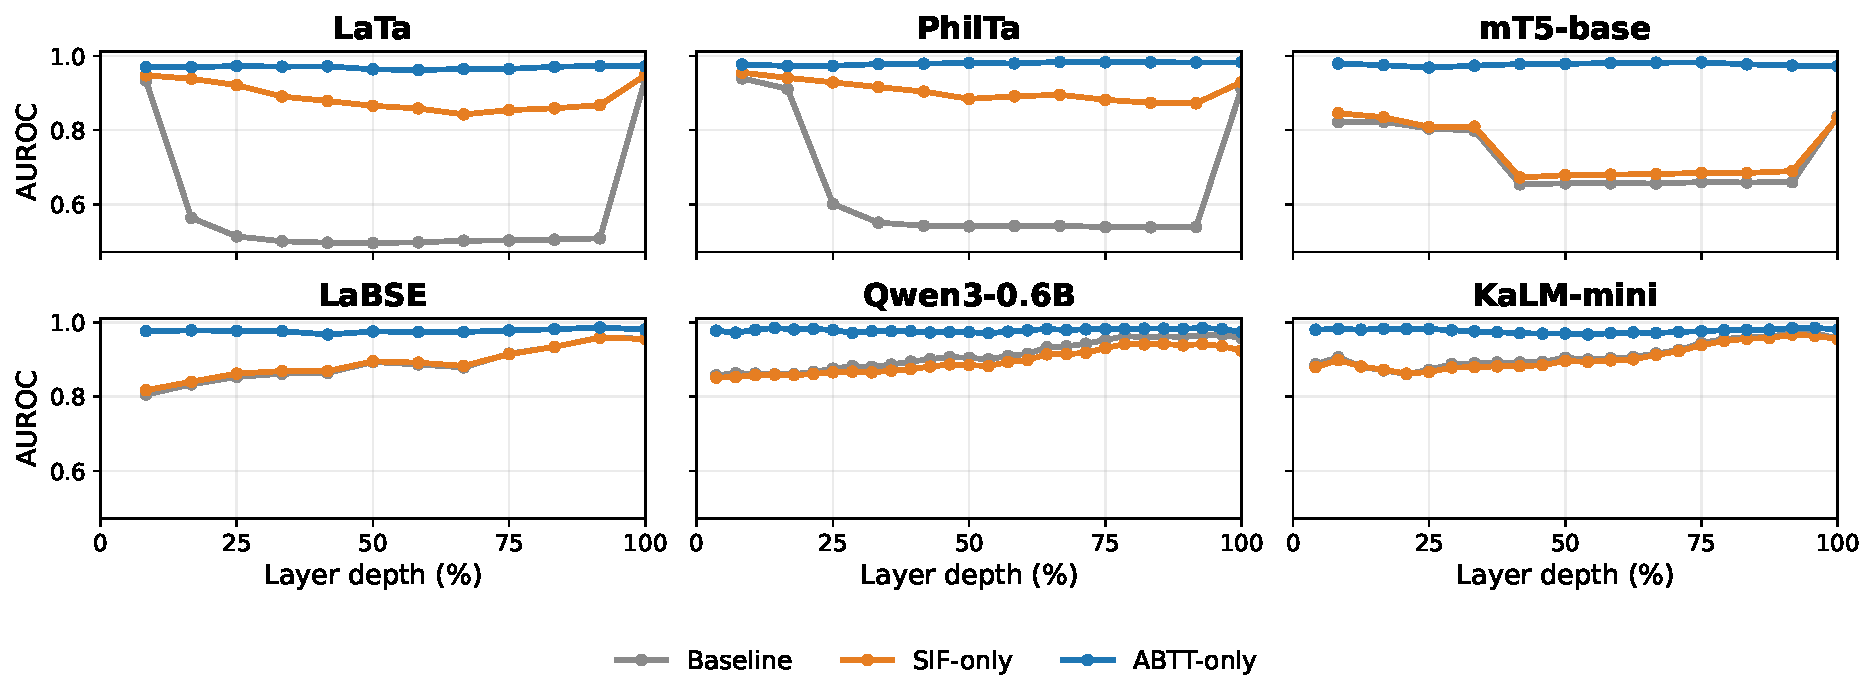
\includegraphics[width=0.96\textwidth]{fig_release_aucroc_6model.pdf}
\caption{Task A AUROC against normalized layer depth, same panels and same series as Figure~\ref{fig:gap}: gray is baseline mean pooling, blue is ABTT-only with $D$ tuned on train, orange is SIF-only. In the top row, LaTa and PhilTa fall to chance in their middle layers and mT5-base loses more than half of its above-chance separation; for mT5-base this panel is the only view of the collapse, since its baseline cosine gap in Figure~\ref{fig:gap} rises over the same layers. The three non-T5 models in the bottom row improve close to monotonically with depth and never fall below 0.80. ABTT holds every model near its ceiling at every depth, so the repair does not depend on the collapse being present.}
\label{fig:dip}
\end{figure*}

\begin{table*}[t]
\centering
\small
\begin{tabular}{lrrrrr}
\toprule
\textbf{Model} & \textbf{Operational layer} & \textbf{Most anisotropic layer} & \textbf{PC1 before} & \textbf{PC1 after} & \textbf{Eff. rank before$\rightarrow$after} \\
\midrule
LaTa & 7 & 8 & 0.956 & 0.036 & 1.34$\rightarrow$168.40 \\
PhilTa & 1 & 6 & 0.862 & 0.039 & 1.83$\rightarrow$155.02 \\
mT5-base & 1 & 5 & 1.000 & 0.044 & 1.00$\rightarrow$151.74 \\
\bottomrule
\end{tabular}
\caption{Most anisotropic layers, by top-PC variance share, and operational attribution layers for the three T5 encoders. PC1 and effective-rank values compare baseline geometry with ABTT-D10 at the most anisotropic layer. Operational layers come from the train-only retrieval rule.}
\label{tab:layer_diagnostics_main}
\end{table*}

Across the main-model layer grid, PC1 dominance and low effective rank are strongly associated with ABTT gains over baseline. These associations explain why ABTT helps, but they do not replace the train-only retrieval rule used for layer selection.

\section{Score Distributions at the Collapsed Retrieval Layer}
\label{app:score_distributions}

Figure~\ref{fig:density} restates the collapse and the repair as score distributions rather than as summary metrics, for the model whose collapse is easiest to read.

\begin{figure}[t]
\centering
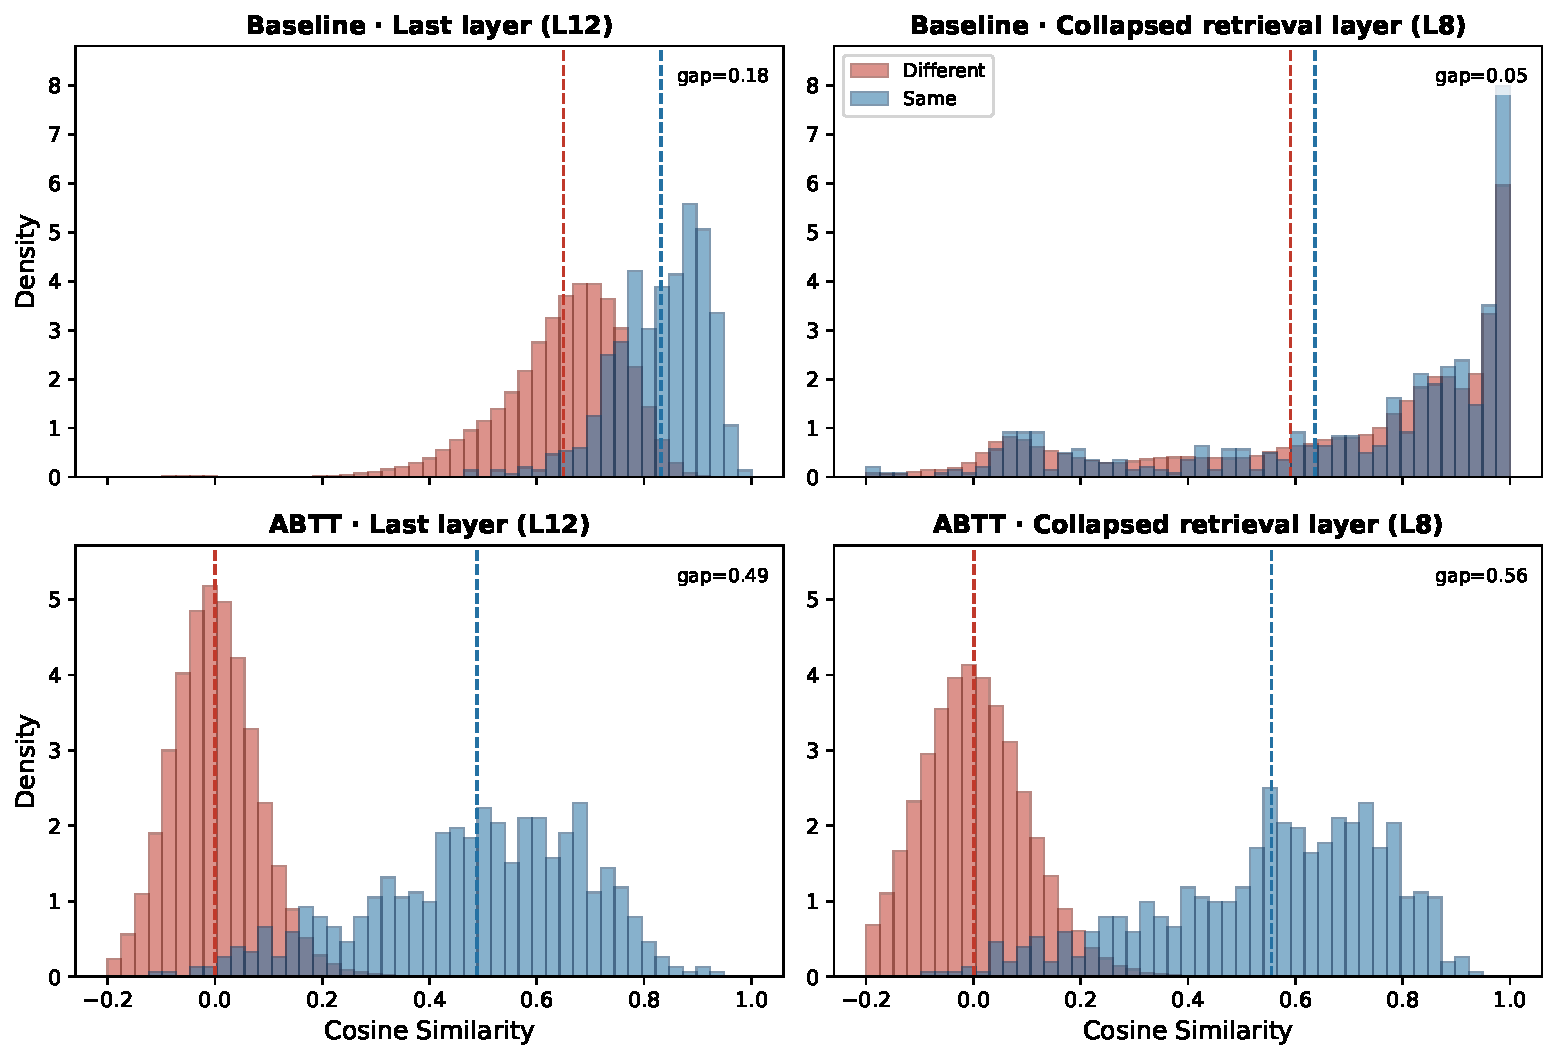
\includegraphics[width=\columnwidth]{paper_fig_density_2x2.pdf}
\caption{Cosine similarity distributions for PhilTa at the last layer and at its collapsed retrieval layer, before and after ABTT. Equivalent pairs share a directory (Same in the legend); non-equivalent pairs do not (Different). The collapsed retrieval layer is layer 8, the layer with the highest training-set AUROC within 30 to 70 percent of encoder depth (layers 4 to 8), so the panel understates the collapse rather than selecting its worst case; the same train-only rule that fixes every other choice in the paper picks it, and its test AUROC is 0.542, close to chance. Two other PhilTa layers carry other meanings and are not shown here: the most anisotropic layer under the top-PC rule of Appendix~\ref{app:layer_diagnostics} is layer 6, and the lowest baseline test AUROC, 0.538, falls at layer 10. Before ABTT the two distributions sit almost on top of each other, and ABTT separates them.}
\label{fig:density}
\end{figure}

\section{Expanded Per-Layer Results for T5 Encoders}
\label{app:per_layer_headline}

The main text compresses the headline retrieval results into Tables~\ref{tab:taskA_headline} and~\ref{tab:taskB_headline}, which report one train-selected layer per model and method. This appendix provides the expanded per-layer Task A duplicate-detection, Task B autonomous-routing, and Task B top-$k$ ranking tables for LaTa, PhilTa, and mT5-base; Appendix~\ref{app:per_layer_extra} gives the same view for the other three models.

\onecolumn
\begin{table*}[t]
\centering
\scriptsize
\setlength{\tabcolsep}{3pt}
\begin{tabular}{llcccc}
\toprule
\multicolumn{2}{c}{} & \multicolumn{4}{c}{\textbf{Task A: Pairwise Duplicate Detection (main)}} \\
\cmidrule(lr){3-6}
\textbf{Model} & \textbf{Layer} & \makecell{AUROC\\(base)} & \makecell{AUROC\\(ABTT)} & \makecell{Cosine gap\\(base)} & \makecell{Cosine gap\\(ABTT)} \\
\midrule
LaTa & 1 & 0.933 & 0.969 & 0.286 & 0.565 \\
 & 2 & 0.565 & 0.969 & 0.020 & 0.553 \\
 & 3 & 0.515 & 0.972 & -0.046 & 0.555 \\
 & 4 & 0.502 & 0.970 & -0.065 & 0.564 \\
 & 5 & 0.498 & 0.971 & -0.068 & 0.572 \\
 & 6 & 0.497 & 0.963 & -0.067 & 0.569 \\
 & 7 & 0.499 & 0.961 & -0.070 & 0.564 \\
 & 8 & 0.504 & 0.964 & -0.073 & 0.558 \\
 & 9 & 0.504 & 0.964 & -0.071 & 0.557 \\
 & 10 & 0.507 & 0.970 & -0.070 & 0.551 \\
 & \textbf{11} & \textbf{0.510} & \textbf{0.973} & \textbf{-0.065} & \textbf{0.550} \\
 & 12 & 0.938 & 0.971 & 0.238 & 0.525 \\
\midrule
PhilTa & 1 & 0.939 & 0.976 & 0.231 & 0.573 \\
 & 2 & 0.911 & 0.971 & 0.161 & 0.551 \\
 & 3 & 0.601 & 0.972 & 0.085 & 0.549 \\
 & 4 & 0.551 & 0.976 & 0.064 & 0.551 \\
 & 5 & 0.543 & 0.978 & 0.054 & 0.551 \\
 & 6 & 0.541 & 0.980 & 0.048 & 0.551 \\
 & 7 & 0.542 & 0.979 & 0.047 & 0.554 \\
 & \textbf{8} & \textbf{0.543} & \textbf{0.983} & \textbf{0.047} & \textbf{0.555} \\
 & 9 & 0.539 & 0.982 & 0.042 & 0.540 \\
 & 10 & 0.539 & 0.982 & 0.040 & 0.530 \\
 & 11 & 0.540 & 0.982 & 0.041 & 0.511 \\
 & 12 & 0.911 & 0.981 & 0.181 & 0.487 \\
\midrule
mT5-base & 1 & 0.823 & 0.979 & 0.027 & 0.550 \\
 & 2 & 0.823 & 0.973 & 0.026 & 0.535 \\
 & 3 & 0.805 & 0.968 & 0.025 & 0.517 \\
 & 4 & 0.800 & 0.975 & 0.040 & 0.503 \\
 & 5 & 0.654 & 0.977 & 0.218 & 0.482 \\
 & 6 & 0.657 & 0.973 & 0.238 & 0.482 \\
 & 7 & 0.657 & 0.979 & 0.243 & 0.482 \\
 & 8 & 0.656 & 0.980 & 0.248 & 0.471 \\
 & \textbf{9} & \textbf{0.660} & \textbf{0.981} & \textbf{0.235} & \textbf{0.475} \\
 & 10 & 0.659 & 0.975 & 0.225 & 0.459 \\
 & 11 & 0.660 & 0.971 & 0.213 & 0.449 \\
 & 12 & 0.839 & 0.970 & 0.082 & 0.441 \\
\bottomrule
\end{tabular}
\caption{Per-layer Task~A pairwise duplicate-detection metrics for the three headline models (LaTa, PhilTa, mT5-base). \texttt{baseline} is mean pooling without correction; \texttt{abtt\_optimal} applies ABTT (no SIF weighting) with $D$ tuned per layer on the train split. Both AUROC and cosine gap are computed over the test n$\times$n cosine matrix with no threshold and no directory routing: AUROC treats same-directory test pairs as positives, and cosine gap is the difference between mean same-directory and mean different-directory cosine. Rows in bold mark the best layer per model, selected by ABTT AUROC.}
\label{tab:taskA_main}
\end{table*}

\begin{table*}[t]
\centering
\scriptsize
\setlength{\tabcolsep}{3pt}
\begin{tabular}{llcccccc}
\toprule
\multicolumn{2}{c}{} & \multicolumn{6}{c}{\textbf{Task B: Autonomous Routing (main, file-level, $\tau$-thresholded)}} \\
\cmidrule(lr){3-8}
\textbf{Model} & \textbf{Layer} & \makecell{Existing\\(base)} & \makecell{Existing\\(ABTT)} & \makecell{New\\(base)} & \makecell{New\\(ABTT)} & \makecell{Overall\\(base)} & \makecell{Overall\\(ABTT)} \\
\midrule
LaTa & \textbf{1} & \textbf{0.630} & \textbf{0.910} & \textbf{0.916} & \textbf{0.907} & \textbf{0.738} & \textbf{0.909} \\
 & 2 & 0.153 & 0.905 & 0.913 & 0.892 & 0.439 & 0.900 \\
 & 3 & 0.256 & 0.882 & 0.842 & 0.950 & 0.477 & 0.908 \\
 & 4 & 0.389 & 0.893 & 0.718 & 0.920 & 0.513 & 0.903 \\
 & 5 & 0.374 & 0.892 & 0.715 & 0.913 & 0.502 & 0.900 \\
 & 6 & 0.378 & 0.884 & 0.712 & 0.913 & 0.503 & 0.895 \\
 & 7 & 0.372 & 0.875 & 0.715 & 0.916 & 0.501 & 0.890 \\
 & 8 & 0.379 & 0.884 & 0.706 & 0.885 & 0.502 & 0.885 \\
 & 9 & 0.366 & 0.886 & 0.724 & 0.873 & 0.501 & 0.881 \\
 & 10 & 0.344 & 0.873 & 0.752 & 0.882 & 0.498 & 0.876 \\
 & 11 & 0.310 & 0.867 & 0.786 & 0.901 & 0.490 & 0.880 \\
 & 12 & 0.576 & 0.890 & 0.932 & 0.833 & 0.710 & 0.868 \\
\midrule
PhilTa & \textbf{1} & \textbf{0.591} & \textbf{0.918} & \textbf{0.904} & \textbf{0.901} & \textbf{0.709} & \textbf{0.911} \\
 & 2 & 0.479 & 0.895 & 0.867 & 0.885 & 0.625 & 0.892 \\
 & 3 & 0.193 & 0.897 & 0.889 & 0.879 & 0.455 & 0.890 \\
 & 4 & 0.148 & 0.886 & 0.923 & 0.873 & 0.439 & 0.881 \\
 & 5 & 0.252 & 0.879 & 0.796 & 0.873 & 0.457 & 0.876 \\
 & 6 & 0.338 & 0.905 & 0.700 & 0.817 & 0.474 & 0.872 \\
 & 7 & 0.301 & 0.901 & 0.746 & 0.830 & 0.469 & 0.874 \\
 & 8 & 0.262 & 0.875 & 0.808 & 0.885 & 0.467 & 0.879 \\
 & 9 & 0.303 & 0.890 & 0.762 & 0.870 & 0.476 & 0.882 \\
 & 10 & 0.299 & 0.908 & 0.780 & 0.793 & 0.480 & 0.865 \\
 & 11 & 0.256 & 0.869 & 0.824 & 0.836 & 0.470 & 0.857 \\
 & 12 & 0.338 & 0.880 & 0.898 & 0.876 & 0.549 & 0.879 \\
\midrule
mT5-base & \textbf{1} & \textbf{0.135} & \textbf{0.877} & \textbf{0.981} & \textbf{0.947} & \textbf{0.453} & \textbf{0.903} \\
 & 2 & 0.110 & 0.890 & 0.975 & 0.910 & 0.436 & 0.897 \\
 & 3 & 0.161 & 0.794 & 0.926 & 0.941 & 0.449 & 0.850 \\
 & 4 & 0.269 & 0.787 & 0.858 & 0.882 & 0.491 & 0.823 \\
 & 5 & 0.422 & 0.746 & 0.659 & 0.864 & 0.512 & 0.790 \\
 & 6 & 0.636 & 0.755 & 0.489 & 0.836 & 0.580 & 0.786 \\
 & 7 & 0.594 & 0.793 & 0.517 & 0.851 & 0.565 & 0.815 \\
 & 8 & 0.557 & 0.809 & 0.560 & 0.842 & 0.558 & 0.822 \\
 & 9 & 0.364 & 0.841 & 0.746 & 0.814 & 0.508 & 0.831 \\
 & 10 & 0.314 & 0.794 & 0.783 & 0.876 & 0.491 & 0.825 \\
 & 11 & 0.297 & 0.763 & 0.780 & 0.854 & 0.479 & 0.797 \\
 & 12 & 0.198 & 0.834 & 0.926 & 0.799 & 0.472 & 0.821 \\
\bottomrule
\end{tabular}
\caption{Per-layer Task~B autonomous routing accuracy for the three headline models. \texttt{baseline} is mean pooling without correction; \texttt{abtt\_optimal} applies ABTT (no SIF weighting) with $D$ tuned per layer on the train split. For every test file we compute $s_i = \max_{j \neq i} \cos(e_i, e_j)$ against the rest of the test set and compare to the learned threshold $\tau$ (fit on train via $F_1$-optimal cut on same-directory vs.\ different-directory pairs). The decision is binary first (existing if $s_i \geq \tau$, else new); only files predicted existing are then routed to their top-1 neighbour's directory. We report \textbf{existing accuracy} (restricted to files whose true partner is in the test set), \textbf{new accuracy} (files that should be flagged as novel), and \textbf{overall assignment accuracy}. Rows in bold mark the best layer per model, selected by ABTT overall assignment accuracy.}
\label{tab:taskB_routing_main}
\end{table*}

\begin{table*}[t]
\centering
\scriptsize
\setlength{\tabcolsep}{3pt}
\begin{tabular}{llcccccc}
\toprule
\multicolumn{2}{c}{} & \multicolumn{6}{c}{\textbf{Task B: Top-K Ranking (main, single-seed v2)}} \\
\cmidrule(lr){3-8}
\textbf{Model} & \textbf{Layer} & \makecell{Acc@1\\(base)} & \makecell{Acc@1\\(ABTT)} & \makecell{Existing\\(base)} & \makecell{Existing\\(ABTT)} & \makecell{New\\(base)} & \makecell{New\\(ABTT)} \\
\midrule
LaTa & 1 & 0.721 & 0.880 & 0.630 & 0.910 & 0.916 & 0.907 \\
 & 2 & 0.383 & 0.869 & 0.153 & 0.905 & 0.913 & 0.892 \\
 & \textbf{3} & \textbf{0.350} & \textbf{0.882} & \textbf{0.256} & \textbf{0.882} & \textbf{0.842} & \textbf{0.950} \\
 & 4 & 0.303 & 0.881 & 0.389 & 0.893 & 0.718 & 0.920 \\
 & 5 & 0.297 & 0.875 & 0.374 & 0.892 & 0.715 & 0.913 \\
 & 6 & 0.297 & 0.874 & 0.378 & 0.884 & 0.712 & 0.913 \\
 & 7 & 0.302 & 0.868 & 0.372 & 0.875 & 0.715 & 0.916 \\
 & 8 & 0.302 & 0.861 & 0.379 & 0.884 & 0.706 & 0.885 \\
 & 9 & 0.309 & 0.858 & 0.366 & 0.886 & 0.724 & 0.873 \\
 & 10 & 0.317 & 0.852 & 0.344 & 0.873 & 0.752 & 0.882 \\
 & 11 & 0.331 & 0.857 & 0.310 & 0.867 & 0.786 & 0.901 \\
 & 12 & 0.689 & 0.841 & 0.576 & 0.890 & 0.932 & 0.833 \\
\midrule
PhilTa & \textbf{1} & \textbf{0.693} & \textbf{0.883} & \textbf{0.591} & \textbf{0.918} & \textbf{0.904} & \textbf{0.901} \\
 & 2 & 0.603 & 0.869 & 0.479 & 0.895 & 0.867 & 0.885 \\
 & 3 & 0.389 & 0.865 & 0.193 & 0.897 & 0.889 & 0.879 \\
 & 4 & 0.369 & 0.859 & 0.148 & 0.886 & 0.923 & 0.873 \\
 & 5 & 0.334 & 0.854 & 0.252 & 0.879 & 0.796 & 0.873 \\
 & 6 & 0.310 & 0.845 & 0.338 & 0.905 & 0.700 & 0.817 \\
 & 7 & 0.325 & 0.847 & 0.301 & 0.901 & 0.746 & 0.830 \\
 & 8 & 0.350 & 0.857 & 0.262 & 0.875 & 0.808 & 0.885 \\
 & 9 & 0.337 & 0.857 & 0.303 & 0.890 & 0.762 & 0.870 \\
 & 10 & 0.344 & 0.833 & 0.299 & 0.908 & 0.780 & 0.793 \\
 & 11 & 0.355 & 0.829 & 0.256 & 0.869 & 0.824 & 0.836 \\
 & 12 & 0.528 & 0.854 & 0.338 & 0.880 & 0.898 & 0.876 \\
\midrule
mT5-base & \textbf{1} & \textbf{0.451} & \textbf{0.885} & \textbf{0.135} & \textbf{0.877} & \textbf{0.981} & \textbf{0.947} \\
 & 2 & 0.435 & 0.874 & 0.110 & 0.890 & 0.975 & 0.910 \\
 & 3 & 0.445 & 0.830 & 0.161 & 0.794 & 0.926 & 0.941 \\
 & 4 & 0.467 & 0.798 & 0.269 & 0.787 & 0.858 & 0.882 \\
 & 5 & 0.352 & 0.756 & 0.422 & 0.746 & 0.659 & 0.864 \\
 & 6 & 0.346 & 0.775 & 0.636 & 0.766 & 0.489 & 0.876 \\
 & 7 & 0.352 & 0.775 & 0.594 & 0.793 & 0.517 & 0.851 \\
 & 8 & 0.366 & 0.784 & 0.557 & 0.809 & 0.560 & 0.842 \\
 & 9 & 0.394 & 0.787 & 0.364 & 0.841 & 0.746 & 0.814 \\
 & 10 & 0.387 & 0.788 & 0.314 & 0.794 & 0.783 & 0.876 \\
 & 11 & 0.378 & 0.765 & 0.297 & 0.763 & 0.780 & 0.854 \\
 & 12 & 0.466 & 0.779 & 0.198 & 0.834 & 0.926 & 0.799 \\
\bottomrule
\end{tabular}
\caption{Per-layer Task~B top-$k$ ranking metrics for the three headline models. \texttt{baseline} is mean pooling without correction; \texttt{abtt\_optimal} applies ABTT (no SIF weighting) with $D$ tuned per layer on the train split. This table is computed on the single-seed v2 split (no $M$-seed averaging, since the mseed sweep was run only for SIF-conditioned variants; see Table~\ref{tab:taskB_ranking_appendix_mseed} for the multi-seed SIF+ABTT view). \textbf{Acc@1} is directory accuracy at rank~1, with an existing/new decomposition. Rows in bold mark the best layer per model, selected by ABTT Acc@1.}
\label{tab:taskB_ranking_main}
\end{table*}

\twocolumn

\section{Last-Token vs.\ Mean Pooling}
\label{app:lasttok}

Decoder-only embedding models often use last-token pooling. We compare last-token pooling with mean pooling under the same ABTT pipeline, train/test split, and ABTT choices. Table~\ref{tab:lasttok_comparison} reports, for each model and pooling, the layer chosen on the train split by directory accuracy at rank 1, the rule of Table~\ref{tab:taskB_headline}, with test-set Task B assignment accuracy, directory accuracy at rank 1, and cosine gap at that layer. Mean pooling performs better on assignment accuracy for every model in this experiment, including the decoder-only models.

\begin{table*}[t]
\centering
\small
\setlength{\tabcolsep}{6pt}
\caption{Mean versus last-token pooling under ABTT with $D$ tuned per layer on the train split, for the five paper models whose last-token embeddings were extracted (mT5-base was not part of this run). For each model and pooling the layer is the one with the highest training-set directory accuracy at rank~1, the rule behind the ABTT subscripts of Table~\ref{tab:taskB_headline}; $D$ is the number of principal components removed at that layer. The three score columns are test-set Task~B assignment accuracy, Task~B directory accuracy at rank~1, and Task~A cosine gap at that layer.}
\label{tab:lasttok_comparison}
\begin{tabular}{llrrccc}
\toprule
Model & Pooling & Layer & $D$ & Assignment acc. & Dir.\ acc.\ @1 & Cosine gap \\
\midrule
LaTa & Mean & 8 & 10 & 0.885 & 0.861 & 0.558 \\
 & Last token & 7 & 10 & 0.664 & 0.466 & 0.308 \\
\midrule
PhilTa & Mean & 1 & 10 & 0.911 & 0.883 & 0.573 \\
 & Last token & 11 & 10 & 0.589 & 0.406 & 0.205 \\
\midrule
LaBSE & Mean & 11 & 10 & 0.908 & 0.885 & 0.610 \\
 & Last token & 12 & 10 & 0.895 & 0.871 & 0.586 \\
\midrule
Qwen3-0.6B & Mean & 5 & 10 & 0.915 & 0.894 & 0.545 \\
 & Last token & 26 & 5 & 0.881 & 0.864 & 0.580 \\
\midrule
KaLM-mini & Mean & 3 & 10 & 0.917 & 0.894 & 0.552 \\
 & Last token & 24 & 10 & 0.875 & 0.847 & 0.483 \\
\bottomrule
\end{tabular}
\end{table*}


\section{Per-Layer Results for Non-T5 Models}
\label{app:per_layer_extra}

The main text focuses on LaTa, PhilTa, and mT5-base. This appendix reports the same per-layer view for LaBSE, Qwen3-0.6B, and KaLM-mini under the same comparison: baseline mean pooling versus ABTT with $D$ tuned per layer on the train split.

\onecolumn
\begingroup
\small
\setlength{\tabcolsep}{4pt}
\begin{longtable}{llcccc}
\caption{Per-layer Task~A pairwise metrics for the remaining three models (LaBSE, Qwen3-0.6B, KaLM-mini), under the same two-method comparison as the main paper. \texttt{baseline} is mean pooling without correction; \texttt{abtt\_optimal} applies ABTT (no SIF weighting) with $D$ tuned per layer on the train split. Both AUROC and cosine gap are computed over the test n$\times$n cosine matrix with no threshold and no directory routing: AUROC treats same-directory test pairs as positives, and cosine gap is the difference between mean same-directory and mean different-directory cosine. Rows in bold mark the best layer per model, selected by ABTT AUROC.}
\label{tab:taskA_appendix} \\
\toprule
\multicolumn{2}{c}{} & \multicolumn{4}{c}{\textbf{Task A: Pairwise Duplicate Detection (appendix models)}} \\
\cmidrule(lr){3-6}
\textbf{Model} & \textbf{Layer} & \makecell{AUROC\\(base)} & \makecell{AUROC\\(ABTT)} & \makecell{Cosine gap\\(base)} & \makecell{Cosine gap\\(ABTT)} \\
\midrule
\endfirsthead
\toprule
\multicolumn{2}{c}{} & \multicolumn{4}{c}{\textbf{Task A: Pairwise Duplicate Detection (appendix models)}} \\
\cmidrule(lr){3-6}
\textbf{Model} & \textbf{Layer} & \makecell{AUROC\\(base)} & \makecell{AUROC\\(ABTT)} & \makecell{Cosine gap\\(base)} & \makecell{Cosine gap\\(ABTT)} \\
\midrule
\endhead
\midrule
\multicolumn{6}{r}{\textit{(continued on next page)}} \\
\endfoot
\bottomrule
\endlastfoot
LaBSE & 1 & 0.807 & 0.976 & 0.060 & 0.519 \\
 & 2 & 0.835 & 0.978 & 0.038 & 0.531 \\
 & 3 & 0.855 & 0.977 & 0.063 & 0.543 \\
 & 4 & 0.864 & 0.976 & 0.074 & 0.525 \\
 & 5 & 0.866 & 0.967 & 0.066 & 0.500 \\
 & 6 & 0.895 & 0.974 & 0.078 & 0.532 \\
 & 7 & 0.889 & 0.973 & 0.089 & 0.523 \\
 & 8 & 0.881 & 0.973 & 0.080 & 0.522 \\
 & 9 & 0.918 & 0.976 & 0.091 & 0.564 \\
 & 10 & 0.936 & 0.980 & 0.103 & 0.584 \\
 & \textbf{11} & \textbf{0.961} & \textbf{0.984} & \textbf{0.061} & \textbf{0.610} \\
 & 12 & 0.957 & 0.979 & 0.183 & 0.592 \\
\midrule
Qwen3-0.6B & 1 & 0.859 & 0.978 & 0.033 & 0.564 \\
 & 2 & 0.864 & 0.972 & 0.024 & 0.553 \\
 & 3 & 0.864 & 0.980 & 0.037 & 0.555 \\
 & \textbf{4} & \textbf{0.861} & \textbf{0.985} & \textbf{0.036} & \textbf{0.546} \\
 & 5 & 0.862 & 0.980 & 0.030 & 0.545 \\
 & 6 & 0.868 & 0.983 & 0.035 & 0.545 \\
 & 7 & 0.877 & 0.980 & 0.033 & 0.544 \\
 & 8 & 0.884 & 0.972 & 0.037 & 0.533 \\
 & 9 & 0.882 & 0.977 & 0.034 & 0.532 \\
 & 10 & 0.888 & 0.976 & 0.031 & 0.530 \\
 & 11 & 0.896 & 0.970 & 0.030 & 0.516 \\
 & 12 & 0.903 & 0.973 & 0.027 & 0.531 \\
 & 13 & 0.908 & 0.974 & 0.026 & 0.524 \\
 & 14 & 0.906 & 0.974 & 0.024 & 0.519 \\
 & 15 & 0.902 & 0.971 & 0.022 & 0.514 \\
 & 16 & 0.911 & 0.975 & 0.026 & 0.509 \\
 & 17 & 0.917 & 0.978 & 0.032 & 0.521 \\
 & 18 & 0.934 & 0.982 & 0.032 & 0.537 \\
 & 19 & 0.937 & 0.980 & 0.035 & 0.541 \\
 & 20 & 0.943 & 0.982 & 0.041 & 0.559 \\
 & 21 & 0.953 & 0.982 & 0.047 & 0.562 \\
 & 22 & 0.963 & 0.983 & 0.044 & 0.583 \\
 & 23 & 0.960 & 0.983 & 0.038 & 0.578 \\
 & 24 & 0.962 & 0.984 & 0.032 & 0.576 \\
 & 25 & 0.960 & 0.983 & 0.027 & 0.578 \\
 & 26 & 0.965 & 0.985 & 0.024 & 0.568 \\
 & 27 & 0.966 & 0.982 & 0.017 & 0.559 \\
 & 28 & 0.958 & 0.975 & 0.098 & 0.556 \\
\midrule
KaLM-mini & 1 & 0.888 & 0.980 & 0.064 & 0.568 \\
 & 2 & 0.908 & 0.983 & 0.044 & 0.566 \\
 & 3 & 0.882 & 0.980 & 0.062 & 0.552 \\
 & 4 & 0.872 & 0.983 & 0.060 & 0.553 \\
 & 5 & 0.862 & 0.982 & 0.062 & 0.541 \\
 & 6 & 0.873 & 0.982 & 0.062 & 0.528 \\
 & 7 & 0.889 & 0.977 & 0.072 & 0.524 \\
 & 8 & 0.891 & 0.975 & 0.072 & 0.523 \\
 & 9 & 0.893 & 0.972 & 0.066 & 0.507 \\
 & 10 & 0.893 & 0.970 & 0.067 & 0.494 \\
 & 11 & 0.895 & 0.969 & 0.061 & 0.474 \\
 & 12 & 0.905 & 0.968 & 0.071 & 0.475 \\
 & 13 & 0.901 & 0.966 & 0.066 & 0.467 \\
 & 14 & 0.904 & 0.970 & 0.063 & 0.471 \\
 & 15 & 0.907 & 0.972 & 0.067 & 0.468 \\
 & 16 & 0.917 & 0.970 & 0.071 & 0.488 \\
 & 17 & 0.926 & 0.973 & 0.075 & 0.501 \\
 & 18 & 0.944 & 0.976 & 0.060 & 0.519 \\
 & 19 & 0.955 & 0.978 & 0.061 & 0.530 \\
 & 20 & 0.959 & 0.979 & 0.054 & 0.554 \\
 & 21 & 0.961 & 0.980 & 0.043 & 0.554 \\
 & 22 & 0.969 & 0.984 & 0.050 & 0.554 \\
 & \textbf{23} & \textbf{0.970} & \textbf{0.985} & \textbf{0.056} & \textbf{0.552} \\
 & 24 & 0.954 & 0.981 & 0.243 & 0.520 \\
\end{longtable}
\endgroup

\begingroup
\small
\setlength{\tabcolsep}{4pt}
\begin{longtable}{llcccccc}
\caption{Per-layer Task~B autonomous routing accuracy for the remaining three models. \texttt{baseline} is mean pooling without correction; \texttt{abtt\_optimal} applies ABTT (no SIF weighting) with $D$ tuned per layer on the train split. For every test file we compute $s_i = \max_{j \neq i} \cos(e_i, e_j)$ against the rest of the test set and compare to the learned threshold $\tau$ (fit on train via $F_1$-optimal cut on same-directory vs.\ different-directory pairs). The decision is binary first (existing if $s_i \geq \tau$, else new); only files predicted existing are then routed to their top-1 neighbour's directory. We report \textbf{existing accuracy} (restricted to files whose true partner is in the test set), \textbf{new accuracy} (files that should be flagged as novel), and \textbf{overall assignment accuracy}. Rows in bold mark the best layer per model, selected by ABTT overall assignment accuracy.}
\label{tab:taskB_routing_appendix} \\
\toprule
\multicolumn{2}{c}{} & \multicolumn{6}{c}{\textbf{Task B: Autonomous Routing (appendix models)}} \\
\cmidrule(lr){3-8}
\textbf{Model} & \textbf{Layer} & \makecell{Existing\\(base)} & \makecell{Existing\\(ABTT)} & \makecell{New\\(base)} & \makecell{New\\(ABTT)} & \makecell{Overall\\(base)} & \makecell{Overall\\(ABTT)} \\
\midrule
\endfirsthead
\toprule
\multicolumn{2}{c}{} & \multicolumn{6}{c}{\textbf{Task B: Autonomous Routing (appendix models)}} \\
\cmidrule(lr){3-8}
\textbf{Model} & \textbf{Layer} & \makecell{Existing\\(base)} & \makecell{Existing\\(ABTT)} & \makecell{New\\(base)} & \makecell{New\\(ABTT)} & \makecell{Overall\\(base)} & \makecell{Overall\\(ABTT)} \\
\midrule
\endhead
\midrule
\multicolumn{8}{r}{\textit{(continued on next page)}} \\
\endfoot
\bottomrule
\endlastfoot
LaBSE & 1 & 0.222 & 0.879 & 0.898 & 0.873 & 0.477 & 0.876 \\
 & 2 & 0.381 & 0.875 & 0.811 & 0.827 & 0.543 & 0.857 \\
 & 3 & 0.277 & 0.886 & 0.907 & 0.867 & 0.514 & 0.879 \\
 & 4 & 0.372 & 0.897 & 0.885 & 0.836 & 0.565 & 0.874 \\
 & 5 & 0.327 & 0.845 & 0.901 & 0.851 & 0.543 & 0.847 \\
 & 6 & 0.548 & 0.860 & 0.882 & 0.851 & 0.674 & 0.857 \\
 & 7 & 0.398 & 0.849 & 0.892 & 0.830 & 0.584 & 0.841 \\
 & 8 & 0.385 & 0.869 & 0.870 & 0.743 & 0.568 & 0.822 \\
 & 9 & 0.421 & 0.871 & 0.929 & 0.817 & 0.612 & 0.851 \\
 & 10 & 0.606 & 0.892 & 0.892 & 0.805 & 0.713 & 0.859 \\
 & \textbf{11} & \textbf{0.785} & \textbf{0.923} & \textbf{0.913} & \textbf{0.882} & \textbf{0.833} & \textbf{0.908} \\
 & 12 & 0.729 & 0.914 & 0.938 & 0.864 & 0.808 & 0.895 \\
\midrule
Qwen3-0.6B & 1 & 0.264 & 0.921 & 0.960 & 0.885 & 0.526 & 0.908 \\
 & 2 & 0.437 & 0.869 & 0.814 & 0.916 & 0.579 & 0.887 \\
 & 3 & 0.250 & 0.914 & 0.947 & 0.907 & 0.513 & 0.911 \\
 & 4 & 0.411 & 0.936 & 0.848 & 0.842 & 0.576 & 0.901 \\
 & \textbf{5} & \textbf{0.181} & \textbf{0.910} & \textbf{0.932} & \textbf{0.923} & \textbf{0.464} & \textbf{0.915} \\
 & 6 & 0.422 & 0.935 & 0.830 & 0.796 & 0.576 & 0.882 \\
 & 7 & 0.250 & 0.890 & 0.947 & 0.876 & 0.513 & 0.885 \\
 & 8 & 0.409 & 0.931 & 0.895 & 0.799 & 0.592 & 0.881 \\
 & 9 & 0.460 & 0.901 & 0.851 & 0.851 & 0.607 & 0.882 \\
 & 10 & 0.533 & 0.892 & 0.836 & 0.864 & 0.647 & 0.881 \\
 & 11 & 0.293 & 0.895 & 0.978 & 0.814 & 0.551 & 0.865 \\
 & 12 & 0.407 & 0.912 & 0.938 & 0.817 & 0.607 & 0.876 \\
 & 13 & 0.432 & 0.908 & 0.944 & 0.836 & 0.625 & 0.881 \\
 & 14 & 0.456 & 0.907 & 0.926 & 0.811 & 0.633 & 0.871 \\
 & 15 & 0.469 & 0.901 & 0.920 & 0.845 & 0.639 & 0.880 \\
 & 16 & 0.639 & 0.897 & 0.830 & 0.808 & 0.711 & 0.864 \\
 & 17 & 0.480 & 0.886 & 0.935 & 0.851 & 0.652 & 0.873 \\
 & 18 & 0.553 & 0.882 & 0.944 & 0.839 & 0.700 & 0.866 \\
 & 19 & 0.514 & 0.871 & 0.966 & 0.858 & 0.684 & 0.866 \\
 & 20 & 0.654 & 0.865 & 0.898 & 0.892 & 0.746 & 0.875 \\
 & 21 & 0.647 & 0.912 & 0.950 & 0.898 & 0.761 & 0.907 \\
 & 22 & 0.731 & 0.888 & 0.938 & 0.916 & 0.809 & 0.899 \\
 & 23 & 0.622 & 0.914 & 0.966 & 0.895 & 0.752 & 0.907 \\
 & 24 & 0.748 & 0.901 & 0.935 & 0.935 & 0.818 & 0.914 \\
 & 25 & 0.574 & 0.893 & 0.975 & 0.923 & 0.725 & 0.904 \\
 & 26 & 0.613 & 0.899 & 0.975 & 0.895 & 0.749 & 0.897 \\
 & 27 & 0.793 & 0.877 & 0.833 & 0.923 & 0.808 & 0.894 \\
 & 28 & 0.796 & 0.877 & 0.867 & 0.913 & 0.823 & 0.890 \\
\midrule
KaLM-mini & \textbf{1} & \textbf{0.391} & \textbf{0.921} & \textbf{0.907} & \textbf{0.920} & \textbf{0.585} & \textbf{0.921} \\
 & 2 & 0.493 & 0.916 & 0.848 & 0.879 & 0.627 & 0.902 \\
 & 3 & 0.443 & 0.923 & 0.870 & 0.907 & 0.604 & 0.917 \\
 & 4 & 0.308 & 0.931 & 0.935 & 0.895 & 0.544 & 0.917 \\
 & 5 & 0.338 & 0.905 & 0.882 & 0.923 & 0.543 & 0.911 \\
 & 6 & 0.256 & 0.895 & 0.910 & 0.920 & 0.502 & 0.904 \\
 & 7 & 0.475 & 0.864 & 0.854 & 0.944 & 0.618 & 0.894 \\
 & 8 & 0.467 & 0.862 & 0.870 & 0.913 & 0.619 & 0.881 \\
 & 9 & 0.469 & 0.873 & 0.885 & 0.870 & 0.626 & 0.872 \\
 & 10 & 0.449 & 0.875 & 0.885 & 0.870 & 0.613 & 0.873 \\
 & 11 & 0.458 & 0.862 & 0.885 & 0.864 & 0.619 & 0.862 \\
 & 12 & 0.507 & 0.862 & 0.895 & 0.904 & 0.653 & 0.878 \\
 & 13 & 0.540 & 0.860 & 0.895 & 0.870 & 0.674 & 0.864 \\
 & 14 & 0.593 & 0.836 & 0.845 & 0.885 & 0.688 & 0.854 \\
 & 15 & 0.566 & 0.864 & 0.898 & 0.827 & 0.691 & 0.850 \\
 & 16 & 0.550 & 0.849 & 0.935 & 0.830 & 0.695 & 0.841 \\
 & 17 & 0.675 & 0.864 & 0.920 & 0.889 & 0.767 & 0.873 \\
 & 18 & 0.697 & 0.875 & 0.960 & 0.898 & 0.796 & 0.883 \\
 & 19 & 0.721 & 0.873 & 0.966 & 0.892 & 0.814 & 0.880 \\
 & 20 & 0.705 & 0.791 & 0.966 & 0.913 & 0.803 & 0.837 \\
 & 21 & 0.727 & 0.811 & 0.966 & 0.926 & 0.817 & 0.854 \\
 & 22 & 0.850 & 0.879 & 0.916 & 0.923 & 0.875 & 0.895 \\
 & 23 & 0.849 & 0.884 & 0.920 & 0.898 & 0.875 & 0.889 \\
 & 24 & 0.787 & 0.892 & 0.944 & 0.867 & 0.846 & 0.882 \\
\end{longtable}
\endgroup

\begingroup
\small
\setlength{\tabcolsep}{4pt}
\begin{longtable}{llcccccc}
\caption{Per-layer Task~B top-$k$ ranking metrics for the remaining three models. \texttt{baseline} is mean pooling without correction; \texttt{abtt\_optimal} applies ABTT (no SIF weighting) with $D$ tuned per layer on the train split. This table is computed on the single-seed v2 split (no $M$-seed averaging, since the mseed sweep was run only for SIF-conditioned variants; see Table~\ref{tab:taskB_ranking_appendix_mseed} for the multi-seed SIF+ABTT view). \textbf{Acc@1} is directory accuracy at rank~1, with an existing/new decomposition. Rows in bold mark the best layer per model, selected by ABTT Acc@1.}
\label{tab:taskB_ranking_appendix} \\
\toprule
\multicolumn{2}{c}{} & \multicolumn{6}{c}{\textbf{Task B: Top-K Ranking (appendix models, single-seed)}} \\
\cmidrule(lr){3-8}
\textbf{Model} & \textbf{Layer} & \makecell{Acc@1\\(base)} & \makecell{Acc@1\\(ABTT)} & \makecell{Existing\\(base)} & \makecell{Existing\\(ABTT)} & \makecell{New\\(base)} & \makecell{New\\(ABTT)} \\
\midrule
\endfirsthead
\toprule
\multicolumn{2}{c}{} & \multicolumn{6}{c}{\textbf{Task B: Top-K Ranking (appendix models, single-seed)}} \\
\cmidrule(lr){3-8}
\textbf{Model} & \textbf{Layer} & \makecell{Acc@1\\(base)} & \makecell{Acc@1\\(ABTT)} & \makecell{Existing\\(base)} & \makecell{Existing\\(ABTT)} & \makecell{New\\(base)} & \makecell{New\\(ABTT)} \\
\midrule
\endhead
\midrule
\multicolumn{8}{r}{\textit{(continued on next page)}} \\
\endfoot
\bottomrule
\endlastfoot
LaBSE & 1 & 0.465 & 0.851 & 0.222 & 0.879 & 0.898 & 0.873 \\
 & 2 & 0.494 & 0.830 & 0.381 & 0.875 & 0.811 & 0.827 \\
 & 3 & 0.500 & 0.848 & 0.277 & 0.886 & 0.907 & 0.867 \\
 & 4 & 0.542 & 0.841 & 0.372 & 0.897 & 0.885 & 0.836 \\
 & 5 & 0.521 & 0.811 & 0.327 & 0.845 & 0.901 & 0.851 \\
 & 6 & 0.640 & 0.831 & 0.548 & 0.860 & 0.882 & 0.851 \\
 & 7 & 0.561 & 0.810 & 0.398 & 0.849 & 0.892 & 0.830 \\
 & 8 & 0.544 & 0.779 & 0.385 & 0.869 & 0.870 & 0.743 \\
 & 9 & 0.608 & 0.823 & 0.421 & 0.871 & 0.929 & 0.817 \\
 & 10 & 0.693 & 0.832 & 0.606 & 0.892 & 0.892 & 0.805 \\
 & \textbf{11} & \textbf{0.815} & \textbf{0.885} & \textbf{0.785} & \textbf{0.923} & \textbf{0.913} & \textbf{0.882} \\
 & 12 & 0.791 & 0.868 & 0.729 & 0.914 & 0.938 & 0.864 \\
\midrule
Qwen3-0.6B & 1 & 0.521 & 0.875 & 0.264 & 0.921 & 0.960 & 0.885 \\
 & 2 & 0.558 & 0.871 & 0.437 & 0.869 & 0.814 & 0.916 \\
 & 3 & 0.508 & 0.890 & 0.250 & 0.914 & 0.947 & 0.907 \\
 & 4 & 0.559 & 0.874 & 0.411 & 0.936 & 0.848 & 0.842 \\
 & 5 & 0.450 & 0.894 & 0.181 & 0.910 & 0.932 & 0.923 \\
 & 6 & 0.551 & 0.858 & 0.422 & 0.935 & 0.830 & 0.796 \\
 & 7 & 0.507 & 0.859 & 0.250 & 0.890 & 0.947 & 0.876 \\
 & 8 & 0.580 & 0.852 & 0.409 & 0.931 & 0.895 & 0.799 \\
 & 9 & 0.587 & 0.852 & 0.460 & 0.901 & 0.851 & 0.851 \\
 & 10 & 0.622 & 0.848 & 0.533 & 0.892 & 0.836 & 0.864 \\
 & 11 & 0.548 & 0.833 & 0.293 & 0.895 & 0.978 & 0.814 \\
 & 12 & 0.603 & 0.848 & 0.407 & 0.912 & 0.938 & 0.817 \\
 & 13 & 0.618 & 0.851 & 0.432 & 0.908 & 0.944 & 0.836 \\
 & 14 & 0.621 & 0.840 & 0.456 & 0.907 & 0.926 & 0.811 \\
 & 15 & 0.627 & 0.848 & 0.469 & 0.901 & 0.920 & 0.845 \\
 & 16 & 0.682 & 0.830 & 0.639 & 0.897 & 0.830 & 0.808 \\
 & 17 & 0.641 & 0.840 & 0.480 & 0.886 & 0.935 & 0.851 \\
 & 18 & 0.691 & 0.837 & 0.553 & 0.882 & 0.944 & 0.839 \\
 & 19 & 0.676 & 0.837 & 0.514 & 0.871 & 0.966 & 0.858 \\
 & 20 & 0.733 & 0.852 & 0.654 & 0.865 & 0.898 & 0.892 \\
 & 21 & 0.752 & 0.881 & 0.647 & 0.912 & 0.950 & 0.898 \\
 & 22 & 0.795 & 0.876 & 0.731 & 0.888 & 0.938 & 0.916 \\
 & 23 & 0.742 & 0.886 & 0.622 & 0.914 & 0.966 & 0.895 \\
 & \textbf{24} & \textbf{0.808} & \textbf{0.896} & \textbf{0.748} & \textbf{0.901} & \textbf{0.935} & \textbf{0.935} \\
 & 25 & 0.718 & 0.886 & 0.574 & 0.893 & 0.975 & 0.923 \\
 & 26 & 0.740 & 0.881 & 0.613 & 0.899 & 0.975 & 0.895 \\
 & 27 & 0.787 & 0.876 & 0.793 & 0.877 & 0.833 & 0.923 \\
 & 28 & 0.803 & 0.872 & 0.796 & 0.877 & 0.867 & 0.913 \\
\midrule
KaLM-mini & \textbf{1} & \textbf{0.577} & \textbf{0.902} & \textbf{0.391} & \textbf{0.921} & \textbf{0.907} & \textbf{0.920} \\
 & 2 & 0.607 & 0.879 & 0.493 & 0.916 & 0.848 & 0.879 \\
 & 3 & 0.587 & 0.894 & 0.443 & 0.923 & 0.870 & 0.907 \\
 & 4 & 0.538 & 0.887 & 0.308 & 0.931 & 0.935 & 0.895 \\
 & 5 & 0.524 & 0.882 & 0.338 & 0.905 & 0.882 & 0.923 \\
 & 6 & 0.490 & 0.876 & 0.256 & 0.895 & 0.910 & 0.920 \\
 & 7 & 0.592 & 0.873 & 0.475 & 0.864 & 0.854 & 0.944 \\
 & 8 & 0.597 & 0.860 & 0.467 & 0.862 & 0.870 & 0.913 \\
 & 9 & 0.601 & 0.843 & 0.469 & 0.873 & 0.885 & 0.870 \\
 & 10 & 0.584 & 0.844 & 0.449 & 0.875 & 0.885 & 0.870 \\
 & 11 & 0.586 & 0.836 & 0.458 & 0.862 & 0.885 & 0.864 \\
 & 12 & 0.622 & 0.850 & 0.507 & 0.862 & 0.895 & 0.904 \\
 & 13 & 0.633 & 0.840 & 0.540 & 0.860 & 0.895 & 0.870 \\
 & 14 & 0.636 & 0.829 & 0.593 & 0.836 & 0.845 & 0.885 \\
 & 15 & 0.650 & 0.817 & 0.566 & 0.864 & 0.898 & 0.827 \\
 & 16 & 0.676 & 0.819 & 0.550 & 0.849 & 0.935 & 0.830 \\
 & 17 & 0.747 & 0.852 & 0.675 & 0.864 & 0.920 & 0.889 \\
 & 18 & 0.777 & 0.865 & 0.697 & 0.875 & 0.960 & 0.898 \\
 & 19 & 0.801 & 0.861 & 0.721 & 0.873 & 0.966 & 0.892 \\
 & 20 & 0.789 & 0.817 & 0.705 & 0.791 & 0.966 & 0.913 \\
 & 21 & 0.802 & 0.831 & 0.727 & 0.811 & 0.966 & 0.926 \\
 & 22 & 0.857 & 0.875 & 0.850 & 0.879 & 0.916 & 0.923 \\
 & 23 & 0.859 & 0.872 & 0.849 & 0.884 & 0.920 & 0.898 \\
 & 24 & 0.833 & 0.858 & 0.787 & 0.892 & 0.944 & 0.867 \\
\end{longtable}
\endgroup

\twocolumn

\section{SIF and Whitening Post-Processing Sweeps}
\label{app:sif_variants}

The main text uses ABTT-only as the paper-facing repair. This appendix reports SIF-only, SIF plus fixed-$D$ ABTT, and SIF plus tuned-$D$ ABTT, and gives the full account of the PCA whitening variant that Section~\ref{sec:postproc} excludes. Table~\ref{tab:taskb} first gives the five-seed cumulative top-$K$ result discussed in the main text, with SIF plus ABTT at each model's train-selected layer. The per-layer tables then keep one primary metric per task so the four-method grid stays readable.

\paragraph{Why whitening is excluded.} PCA whitening \citep{su2021whitening} leaves the different-directory cosine mean at or below 0.015, so the learned threshold degenerates: across all 100 whitening cells every file is routed to an existing directory, existing accuracy is 1.000, new accuracy never exceeds one file in 323, and assignment accuracy sits at the 62.4 percent class prior. That prior beats baseline in 60 of 100 cells while directory accuracy at rank 1 never exceeds 0.415, so the apparent gain is a thresholding artifact. SIF and whitening fall short of ABTT for different reasons. SIF acts before pooling, so it can only attenuate the frequent tokens that feed the dominant direction, and whatever survives that reweighting is still pooled into the passage vector; whitening acts after pooling but rescales all directions instead of deleting the top few, which flattens the same-directory margin along with the common component and so degenerates the routing threshold.

% generated table
\begin{table*}[t]
\centering
\small
\setlength{\tabcolsep}{6pt}
\begin{tabular}{lrrrrr}
\toprule
\textbf{Model} & \textbf{Top-1} & \textbf{Top-2} & \textbf{Top-3} & \textbf{Top-4} & \textbf{Top-5} \\
\midrule
LaTa       & 88.9 $\pm$ 0.5 & 96.1 $\pm$ 0.5 & 97.4 $\pm$ 0.6 & 97.9 $\pm$ 0.3 & 98.2 $\pm$ 0.2 \\
PhilTa     & 89.8 $\pm$ 0.8 & 95.8 $\pm$ 0.6 & 97.4 $\pm$ 0.3 & 97.7 $\pm$ 0.3 & 97.8 $\pm$ 0.4 \\
mT5-base   & 89.3 $\pm$ 0.5 & 95.1 $\pm$ 0.2 & 96.7 $\pm$ 0.7 & 97.1 $\pm$ 0.4 & 97.2 $\pm$ 0.4 \\
LaBSE      & 90.6 $\pm$ 1.0 & 95.5 $\pm$ 0.5 & 96.4 $\pm$ 0.5 & 97.2 $\pm$ 0.6 & 97.8 $\pm$ 0.5 \\
Qwen3-0.6B & 89.3 $\pm$ 0.7 & 95.7 $\pm$ 0.4 & 97.1 $\pm$ 0.3 & 97.5 $\pm$ 0.4 & 97.6 $\pm$ 0.4 \\
KaLM-mini  & 89.3 $\pm$ 0.5 & 95.1 $\pm$ 0.4 & 96.6 $\pm$ 0.7 & 97.2 $\pm$ 0.7 & 97.6 $\pm$ 0.5 \\
\bottomrule
\end{tabular}
\caption{Cumulative top-$K$ accuracy for Task B under SIF+ABTT, as mean $\pm$ standard deviation over five query/reference reseedings at a fixed split. For each model the reported layer is chosen on the train split: the layer with the highest training-set directory accuracy at rank~1 for SIF+ABTT in the single-seed run, the same layer as the SIF+ABTT subscript in Table~\ref{tab:taskB_headline}. $D$ is tuned per layer on the train split. This is not always the layer with the highest five-seed mean. Each row is the bold row of Table~\ref{tab:taskB_ranking_appendix_mseed}. Each cell is the percentage of test queries whose labelled directory appears within the top $K$ options. Per-layer top-$k$ rankings: Appendix Tables~\ref{tab:taskB_ranking_main}, \ref{tab:taskB_ranking_appendix}, and~\ref{tab:taskB_ranking_appendix_mseed}.}
\label{tab:taskb}
\end{table*}


\onecolumn
\begingroup
\small
\setlength{\tabcolsep}{4pt}
\begin{longtable}{llcccc}
\caption{Per-layer Task~A AUROC across the SIF-conditioned post-processing suite for all six models. \texttt{sif\_only} replaces mean pooling with SIF-weighted pooling; \texttt{sif\_abtt\_fixed} adds ABTT with fixed $D{=}10$; \texttt{sif\_abtt\_optimal} tunes $D$ per layer on the train split. Gap is omitted to keep the table narrow; the pure-ABTT comparison (not SIF-conditioned) is in Tables~\ref{tab:taskA_main} and~\ref{tab:taskA_appendix}. Rows in bold mark the best layer per model, selected by SIF+ABTT (D-tuned) AUROC.}
\label{tab:taskA_appendix_sif} \\
\toprule
\multicolumn{2}{c}{} & \multicolumn{4}{c}{\textbf{Task A: SIF-suite AUROC (appendix)}} \\
\cmidrule(lr){3-6}
\textbf{Model} & \textbf{Layer} & \makecell{AUROC\\(base)} & \makecell{AUROC\\(SIF)} & \makecell{AUROC\\(SIF+ABTT$_{10}$)} & \makecell{AUROC\\(SIF+ABTT)} \\
\midrule
\endfirsthead
\toprule
\multicolumn{2}{c}{} & \multicolumn{4}{c}{\textbf{Task A: SIF-suite AUROC (appendix)}} \\
\cmidrule(lr){3-6}
\textbf{Model} & \textbf{Layer} & \makecell{AUROC\\(base)} & \makecell{AUROC\\(SIF)} & \makecell{AUROC\\(SIF+ABTT$_{10}$)} & \makecell{AUROC\\(SIF+ABTT)} \\
\midrule
\endhead
\midrule
\multicolumn{6}{r}{\textit{(continued on next page)}} \\
\endfoot
\bottomrule
\endlastfoot
LaTa & \textbf{1} & \textbf{0.934} & \textbf{0.948} & \textbf{0.972} & \textbf{0.976} \\
 & 2 & 0.563 & 0.938 & 0.964 & 0.971 \\
 & 3 & 0.513 & 0.921 & 0.967 & 0.966 \\
 & 4 & 0.500 & 0.890 & 0.970 & 0.968 \\
 & 5 & 0.496 & 0.878 & 0.970 & 0.970 \\
 & 6 & 0.496 & 0.865 & 0.965 & 0.965 \\
 & 7 & 0.498 & 0.858 & 0.966 & 0.966 \\
 & 8 & 0.502 & 0.842 & 0.964 & 0.964 \\
 & 9 & 0.503 & 0.854 & 0.964 & 0.964 \\
 & 10 & 0.505 & 0.859 & 0.966 & 0.966 \\
 & 11 & 0.508 & 0.867 & 0.965 & 0.965 \\
 & 12 & 0.938 & 0.948 & 0.963 & 0.963 \\
\midrule
PhilTa & 1 & 0.939 & 0.955 & 0.975 & 0.975 \\
 & 2 & 0.911 & 0.941 & 0.973 & 0.973 \\
 & 3 & 0.601 & 0.928 & 0.968 & 0.968 \\
 & 4 & 0.551 & 0.916 & 0.972 & 0.972 \\
 & 5 & 0.542 & 0.904 & 0.972 & 0.972 \\
 & 6 & 0.541 & 0.884 & 0.981 & 0.981 \\
 & 7 & 0.542 & 0.891 & 0.981 & 0.981 \\
 & \textbf{8} & \textbf{0.542} & \textbf{0.895} & \textbf{0.982} & \textbf{0.982} \\
 & 9 & 0.539 & 0.881 & 0.977 & 0.977 \\
 & 10 & 0.538 & 0.874 & 0.977 & 0.977 \\
 & 11 & 0.539 & 0.872 & 0.979 & 0.979 \\
 & 12 & 0.911 & 0.929 & 0.969 & 0.969 \\
\midrule
mT5-base & \textbf{1} & \textbf{0.822} & \textbf{0.845} & \textbf{0.974} & \textbf{0.974} \\
 & 2 & 0.822 & 0.835 & 0.966 & 0.966 \\
 & 3 & 0.804 & 0.808 & 0.958 & 0.958 \\
 & 4 & 0.799 & 0.809 & 0.966 & 0.966 \\
 & 5 & 0.654 & 0.672 & 0.974 & 0.974 \\
 & 6 & 0.657 & 0.678 & 0.971 & 0.971 \\
 & 7 & 0.656 & 0.680 & 0.967 & 0.967 \\
 & 8 & 0.656 & 0.681 & 0.968 & 0.968 \\
 & 9 & 0.660 & 0.685 & 0.967 & 0.967 \\
 & 10 & 0.659 & 0.684 & 0.966 & 0.966 \\
 & 11 & 0.659 & 0.689 & 0.966 & 0.966 \\
 & 12 & 0.838 & 0.833 & 0.970 & 0.970 \\
\midrule
LaBSE & 1 & 0.806 & 0.818 & 0.974 & 0.974 \\
 & 2 & 0.833 & 0.840 & 0.975 & 0.975 \\
 & 3 & 0.853 & 0.862 & 0.968 & 0.968 \\
 & 4 & 0.862 & 0.869 & 0.966 & 0.966 \\
 & 5 & 0.864 & 0.869 & 0.964 & 0.964 \\
 & 6 & 0.894 & 0.895 & 0.965 & 0.965 \\
 & 7 & 0.887 & 0.892 & 0.964 & 0.964 \\
 & 8 & 0.879 & 0.883 & 0.968 & 0.968 \\
 & 9 & 0.916 & 0.915 & 0.973 & 0.973 \\
 & 10 & 0.934 & 0.934 & 0.976 & 0.976 \\
 & 11 & 0.960 & 0.959 & 0.983 & 0.983 \\
 & \textbf{12} & \textbf{0.956} & \textbf{0.956} & \textbf{0.980} & \textbf{0.984} \\
\midrule
Qwen3-0.6B & \textbf{1} & \textbf{0.858} & \textbf{0.852} & \textbf{0.982} & \textbf{0.981} \\
 & 2 & 0.863 & 0.853 & 0.972 & 0.972 \\
 & 3 & 0.862 & 0.858 & 0.977 & 0.975 \\
 & 4 & 0.860 & 0.860 & 0.976 & 0.977 \\
 & 5 & 0.861 & 0.858 & 0.971 & 0.971 \\
 & 6 & 0.867 & 0.861 & 0.974 & 0.974 \\
 & 7 & 0.876 & 0.866 & 0.971 & 0.971 \\
 & 8 & 0.882 & 0.868 & 0.969 & 0.969 \\
 & 9 & 0.881 & 0.866 & 0.968 & 0.968 \\
 & 10 & 0.887 & 0.870 & 0.966 & 0.966 \\
 & 11 & 0.895 & 0.875 & 0.964 & 0.964 \\
 & 12 & 0.901 & 0.881 & 0.966 & 0.966 \\
 & 13 & 0.907 & 0.887 & 0.967 & 0.967 \\
 & 14 & 0.905 & 0.885 & 0.966 & 0.966 \\
 & 15 & 0.901 & 0.883 & 0.968 & 0.968 \\
 & 16 & 0.910 & 0.894 & 0.965 & 0.965 \\
 & 17 & 0.916 & 0.899 & 0.967 & 0.974 \\
 & 18 & 0.933 & 0.914 & 0.966 & 0.973 \\
 & 19 & 0.936 & 0.915 & 0.966 & 0.976 \\
 & 20 & 0.943 & 0.918 & 0.971 & 0.977 \\
 & 21 & 0.953 & 0.931 & 0.971 & 0.971 \\
 & 22 & 0.963 & 0.942 & 0.973 & 0.973 \\
 & 23 & 0.961 & 0.941 & 0.973 & 0.973 \\
 & 24 & 0.963 & 0.943 & 0.976 & 0.974 \\
 & 25 & 0.961 & 0.938 & 0.978 & 0.975 \\
 & 26 & 0.966 & 0.942 & 0.980 & 0.980 \\
 & 27 & 0.967 & 0.936 & 0.978 & 0.978 \\
 & 28 & 0.958 & 0.925 & 0.968 & 0.968 \\
\midrule
KaLM-mini & 1 & 0.887 & 0.880 & 0.982 & 0.980 \\
 & 2 & 0.906 & 0.899 & 0.981 & 0.981 \\
 & 3 & 0.881 & 0.882 & 0.977 & 0.977 \\
 & 4 & 0.871 & 0.873 & 0.974 & 0.974 \\
 & 5 & 0.861 & 0.862 & 0.971 & 0.971 \\
 & 6 & 0.872 & 0.867 & 0.967 & 0.967 \\
 & 7 & 0.888 & 0.879 & 0.972 & 0.972 \\
 & 8 & 0.890 & 0.880 & 0.973 & 0.975 \\
 & 9 & 0.892 & 0.882 & 0.968 & 0.968 \\
 & 10 & 0.893 & 0.882 & 0.964 & 0.964 \\
 & 11 & 0.894 & 0.885 & 0.969 & 0.969 \\
 & 12 & 0.905 & 0.896 & 0.966 & 0.966 \\
 & 13 & 0.900 & 0.894 & 0.964 & 0.964 \\
 & 14 & 0.904 & 0.898 & 0.970 & 0.970 \\
 & 15 & 0.907 & 0.901 & 0.970 & 0.970 \\
 & 16 & 0.917 & 0.913 & 0.967 & 0.967 \\
 & 17 & 0.926 & 0.923 & 0.968 & 0.968 \\
 & 18 & 0.945 & 0.939 & 0.977 & 0.977 \\
 & 19 & 0.956 & 0.950 & 0.978 & 0.978 \\
 & 20 & 0.960 & 0.956 & 0.978 & 0.978 \\
 & 21 & 0.962 & 0.958 & 0.980 & 0.983 \\
 & 22 & 0.971 & 0.967 & 0.983 & 0.984 \\
 & \textbf{23} & \textbf{0.972} & \textbf{0.964} & \textbf{0.986} & \textbf{0.985} \\
 & 24 & 0.956 & 0.956 & 0.976 & 0.976 \\
\end{longtable}
\endgroup

\begingroup
\small
\setlength{\tabcolsep}{4pt}
\begin{longtable}{llcccc}
\caption{Per-layer Task~B overall assignment accuracy across the SIF-conditioned suite for all six models. Restricted to overall routing accuracy (existing/new decomposition omitted) to keep the table compact; see Tables~\ref{tab:taskB_routing_main} and~\ref{tab:taskB_routing_appendix} for the pure-ABTT pairwise comparison with existing/new broken out. Rows in bold mark the best layer per model, selected by SIF+ABTT (D-tuned) overall assignment accuracy.}
\label{tab:taskB_routing_appendix_sif} \\
\toprule
\multicolumn{2}{c}{} & \multicolumn{4}{c}{\textbf{Task B: SIF-suite routing (appendix)}} \\
\cmidrule(lr){3-6}
\textbf{Model} & \textbf{Layer} & \makecell{Overall\\(base)} & \makecell{Overall\\(SIF)} & \makecell{Overall\\(SIF+ABTT$_{10}$)} & \makecell{Overall\\(SIF+ABTT)} \\
\midrule
\endfirsthead
\toprule
\multicolumn{2}{c}{} & \multicolumn{4}{c}{\textbf{Task B: SIF-suite routing (appendix)}} \\
\cmidrule(lr){3-6}
\textbf{Model} & \textbf{Layer} & \makecell{Overall\\(base)} & \makecell{Overall\\(SIF)} & \makecell{Overall\\(SIF+ABTT$_{10}$)} & \makecell{Overall\\(SIF+ABTT)} \\
\midrule
\endhead
\midrule
\multicolumn{6}{r}{\textit{(continued on next page)}} \\
\endfoot
\bottomrule
\endlastfoot
LaTa & 1 & 0.738 & 0.832 & 0.920 & 0.899 \\
 & 2 & 0.439 & 0.791 & 0.904 & 0.900 \\
 & \textbf{3} & \textbf{0.477} & \textbf{0.720} & \textbf{0.910} & \textbf{0.907} \\
 & 4 & 0.513 & 0.668 & 0.900 & 0.902 \\
 & 5 & 0.502 & 0.648 & 0.906 & 0.906 \\
 & 6 & 0.503 & 0.668 & 0.895 & 0.895 \\
 & 7 & 0.501 & 0.642 & 0.903 & 0.903 \\
 & 8 & 0.502 & 0.614 & 0.892 & 0.892 \\
 & 9 & 0.501 & 0.618 & 0.889 & 0.889 \\
 & 10 & 0.498 & 0.655 & 0.890 & 0.890 \\
 & 11 & 0.490 & 0.621 & 0.880 & 0.880 \\
 & 12 & 0.710 & 0.804 & 0.902 & 0.902 \\
\midrule
PhilTa & \textbf{1} & \textbf{0.709} & \textbf{0.790} & \textbf{0.914} & \textbf{0.914} \\
 & 2 & 0.625 & 0.738 & 0.892 & 0.892 \\
 & 3 & 0.455 & 0.713 & 0.892 & 0.892 \\
 & 4 & 0.439 & 0.663 & 0.886 & 0.886 \\
 & 5 & 0.457 & 0.626 & 0.899 & 0.899 \\
 & 6 & 0.474 & 0.612 & 0.906 & 0.906 \\
 & 7 & 0.469 & 0.625 & 0.906 & 0.906 \\
 & 8 & 0.467 & 0.614 & 0.886 & 0.886 \\
 & 9 & 0.476 & 0.590 & 0.895 & 0.895 \\
 & 10 & 0.480 & 0.580 & 0.888 & 0.888 \\
 & 11 & 0.470 & 0.565 & 0.886 & 0.886 \\
 & 12 & 0.549 & 0.667 & 0.899 & 0.899 \\
\midrule
mT5-base & \textbf{1} & \textbf{0.453} & \textbf{0.545} & \textbf{0.907} & \textbf{0.907} \\
 & 2 & 0.436 & 0.537 & 0.903 & 0.903 \\
 & 3 & 0.449 & 0.568 & 0.885 & 0.885 \\
 & 4 & 0.491 & 0.488 & 0.857 & 0.857 \\
 & 5 & 0.512 & 0.483 & 0.826 & 0.826 \\
 & 6 & 0.580 & 0.558 & 0.817 & 0.817 \\
 & 7 & 0.565 & 0.554 & 0.832 & 0.832 \\
 & 8 & 0.558 & 0.548 & 0.834 & 0.834 \\
 & 9 & 0.508 & 0.495 & 0.845 & 0.845 \\
 & 10 & 0.491 & 0.495 & 0.832 & 0.832 \\
 & 11 & 0.479 & 0.484 & 0.816 & 0.816 \\
 & 12 & 0.472 & 0.541 & 0.858 & 0.858 \\
\midrule
LaBSE & 1 & 0.477 & 0.521 & 0.886 & 0.886 \\
 & 2 & 0.543 & 0.508 & 0.875 & 0.875 \\
 & 3 & 0.514 & 0.577 & 0.860 & 0.860 \\
 & 4 & 0.565 & 0.587 & 0.869 & 0.869 \\
 & 5 & 0.543 & 0.598 & 0.857 & 0.857 \\
 & 6 & 0.674 & 0.648 & 0.872 & 0.872 \\
 & 7 & 0.584 & 0.634 & 0.858 & 0.858 \\
 & 8 & 0.568 & 0.571 & 0.854 & 0.854 \\
 & 9 & 0.612 & 0.613 & 0.859 & 0.859 \\
 & 10 & 0.713 & 0.698 & 0.864 & 0.864 \\
 & \textbf{11} & \textbf{0.833} & \textbf{0.807} & \textbf{0.896} & \textbf{0.896} \\
 & 12 & 0.808 & 0.834 & 0.890 & 0.880 \\
\midrule
Qwen3-0.6B & 1 & 0.526 & 0.566 & 0.914 & 0.909 \\
 & 2 & 0.579 & 0.524 & 0.894 & 0.894 \\
 & 3 & 0.513 & 0.537 & 0.904 & 0.901 \\
 & 4 & 0.576 & 0.531 & 0.899 & 0.904 \\
 & 5 & 0.464 & 0.537 & 0.908 & 0.908 \\
 & 6 & 0.576 & 0.526 & 0.906 & 0.906 \\
 & \textbf{7} & \textbf{0.513} & \textbf{0.573} & \textbf{0.911} & \textbf{0.911} \\
 & 8 & 0.592 & 0.627 & 0.911 & 0.911 \\
 & 9 & 0.607 & 0.576 & 0.910 & 0.910 \\
 & 10 & 0.647 & 0.599 & 0.900 & 0.900 \\
 & 11 & 0.551 & 0.606 & 0.893 & 0.893 \\
 & 12 & 0.607 & 0.663 & 0.900 & 0.900 \\
 & 13 & 0.625 & 0.675 & 0.897 & 0.897 \\
 & 14 & 0.633 & 0.571 & 0.893 & 0.893 \\
 & 15 & 0.639 & 0.600 & 0.893 & 0.893 \\
 & 16 & 0.711 & 0.679 & 0.880 & 0.880 \\
 & 17 & 0.652 & 0.686 & 0.900 & 0.876 \\
 & 18 & 0.700 & 0.731 & 0.899 & 0.882 \\
 & 19 & 0.684 & 0.700 & 0.886 & 0.850 \\
 & 20 & 0.746 & 0.676 & 0.882 & 0.866 \\
 & 21 & 0.761 & 0.739 & 0.892 & 0.892 \\
 & 22 & 0.809 & 0.719 & 0.893 & 0.893 \\
 & 23 & 0.752 & 0.759 & 0.893 & 0.893 \\
 & 24 & 0.818 & 0.706 & 0.900 & 0.899 \\
 & 25 & 0.725 & 0.748 & 0.897 & 0.893 \\
 & 26 & 0.749 & 0.772 & 0.903 & 0.903 \\
 & 27 & 0.808 & 0.760 & 0.899 & 0.899 \\
 & 28 & 0.823 & 0.774 & 0.890 & 0.890 \\
\midrule
KaLM-mini & \textbf{1} & \textbf{0.585} & \textbf{0.604} & \textbf{0.906} & \textbf{0.908} \\
 & 2 & 0.627 & 0.594 & 0.908 & 0.908 \\
 & 3 & 0.604 & 0.576 & 0.907 & 0.907 \\
 & 4 & 0.544 & 0.577 & 0.901 & 0.901 \\
 & 5 & 0.543 & 0.533 & 0.897 & 0.897 \\
 & 6 & 0.502 & 0.558 & 0.900 & 0.900 \\
 & 7 & 0.618 & 0.593 & 0.901 & 0.901 \\
 & 8 & 0.619 & 0.607 & 0.892 & 0.878 \\
 & 9 & 0.626 & 0.663 & 0.876 & 0.876 \\
 & 10 & 0.613 & 0.603 & 0.866 & 0.866 \\
 & 11 & 0.619 & 0.627 & 0.874 & 0.874 \\
 & 12 & 0.653 & 0.642 & 0.874 & 0.874 \\
 & 13 & 0.674 & 0.666 & 0.864 & 0.864 \\
 & 14 & 0.688 & 0.648 & 0.861 & 0.861 \\
 & 15 & 0.691 & 0.698 & 0.866 & 0.866 \\
 & 16 & 0.695 & 0.738 & 0.859 & 0.859 \\
 & 17 & 0.767 & 0.763 & 0.882 & 0.882 \\
 & 18 & 0.796 & 0.796 & 0.879 & 0.879 \\
 & 19 & 0.814 & 0.804 & 0.878 & 0.878 \\
 & 20 & 0.803 & 0.821 & 0.876 & 0.876 \\
 & 21 & 0.817 & 0.832 & 0.874 & 0.876 \\
 & 22 & 0.875 & 0.857 & 0.876 & 0.876 \\
 & 23 & 0.875 & 0.862 & 0.880 & 0.881 \\
 & 24 & 0.846 & 0.847 & 0.869 & 0.869 \\
\end{longtable}
\endgroup

\begingroup
\small
\setlength{\tabcolsep}{4pt}
\begin{longtable}{llcccccc}
\caption{Per-layer Task~B top-$k$ ranking accuracy across all six models, averaged over $M=5$ query/reference reseedings of the v2 train/test split (mean $\pm$ std). \texttt{sif\_abtt\_optimal} applies SIF weighting plus ABTT with $D$ tuned per layer on the train split; the mseed sweep was not run for the pure \texttt{abtt\_optimal} variant reported in the main paper, so we include this table to give a variance-aware view of the SIF-conditioned best variant. Overall assignment accuracy coincides with Acc@1 in the mseed pipeline, so we report the existing/new decomposition instead. Rows in bold mark the best layer per model, selected by SIF+ABTT Acc@1.}
\label{tab:taskB_ranking_appendix_mseed} \\
\toprule
\multicolumn{2}{c}{} & \multicolumn{6}{c}{\textbf{Task B: Top-K Ranking (appendix, 5-seed mean $\pm$ std, SIF+ABTT)}} \\
\cmidrule(lr){3-8}
\textbf{Model} & \textbf{Layer} & \makecell{Acc@1\\(base)} & \makecell{Acc@1\\(SIF+ABTT)} & \makecell{Existing\\(base)} & \makecell{Existing\\(SIF+ABTT)} & \makecell{New\\(base)} & \makecell{New\\(SIF+ABTT)} \\
\midrule
\endfirsthead
\toprule
\multicolumn{2}{c}{} & \multicolumn{6}{c}{\textbf{Task B: Top-K Ranking (appendix, 5-seed mean $\pm$ std, SIF+ABTT)}} \\
\cmidrule(lr){3-8}
\textbf{Model} & \textbf{Layer} & \makecell{Acc@1\\(base)} & \makecell{Acc@1\\(SIF+ABTT)} & \makecell{Existing\\(base)} & \makecell{Existing\\(SIF+ABTT)} & \makecell{New\\(base)} & \makecell{New\\(SIF+ABTT)} \\
\midrule
\endhead
\midrule
\multicolumn{8}{r}{\textit{(continued on next page)}} \\
\endfoot
\bottomrule
\endlastfoot
LaTa & 1 & 0.731 $\pm$ 0.010 & 0.889 $\pm$ 0.010 & 0.563 $\pm$ 0.007 & 0.844 $\pm$ 0.011 & 0.949 $\pm$ 0.011 & 0.948 $\pm$ 0.010 \\
 & 2 & 0.429 $\pm$ 0.011 & 0.888 $\pm$ 0.007 & 0.049 $\pm$ 0.006 & 0.841 $\pm$ 0.007 & 0.920 $\pm$ 0.008 & 0.948 $\pm$ 0.007 \\
 & 3 & 0.393 $\pm$ 0.011 & 0.891 $\pm$ 0.010 & 0.047 $\pm$ 0.006 & 0.847 $\pm$ 0.010 & 0.840 $\pm$ 0.020 & 0.947 $\pm$ 0.012 \\
 & 4 & 0.331 $\pm$ 0.019 & 0.889 $\pm$ 0.009 & 0.048 $\pm$ 0.009 & 0.860 $\pm$ 0.009 & 0.696 $\pm$ 0.030 & 0.925 $\pm$ 0.013 \\
 & 5 & 0.326 $\pm$ 0.021 & 0.891 $\pm$ 0.009 & 0.038 $\pm$ 0.005 & 0.858 $\pm$ 0.008 & 0.698 $\pm$ 0.028 & 0.934 $\pm$ 0.014 \\
 & 6 & 0.322 $\pm$ 0.018 & 0.891 $\pm$ 0.009 & 0.038 $\pm$ 0.007 & 0.863 $\pm$ 0.010 & 0.688 $\pm$ 0.026 & 0.927 $\pm$ 0.013 \\
 & \textbf{7} & \textbf{0.328 $\pm$ 0.020} & \textbf{0.896 $\pm$ 0.008} & \textbf{0.045 $\pm$ 0.007} & \textbf{0.848 $\pm$ 0.009} & \textbf{0.693 $\pm$ 0.028} & \textbf{0.957 $\pm$ 0.010} \\
 & 8 & 0.325 $\pm$ 0.022 & 0.884 $\pm$ 0.008 & 0.046 $\pm$ 0.010 & 0.834 $\pm$ 0.008 & 0.685 $\pm$ 0.032 & 0.949 $\pm$ 0.011 \\
 & 9 & 0.332 $\pm$ 0.019 & 0.886 $\pm$ 0.011 & 0.045 $\pm$ 0.010 & 0.848 $\pm$ 0.009 & 0.701 $\pm$ 0.024 & 0.935 $\pm$ 0.015 \\
 & 10 & 0.346 $\pm$ 0.017 & 0.889 $\pm$ 0.004 & 0.045 $\pm$ 0.010 & 0.846 $\pm$ 0.008 & 0.735 $\pm$ 0.021 & 0.944 $\pm$ 0.012 \\
 & 11 & 0.361 $\pm$ 0.018 & 0.882 $\pm$ 0.009 & 0.045 $\pm$ 0.009 & 0.862 $\pm$ 0.010 & 0.767 $\pm$ 0.029 & 0.907 $\pm$ 0.014 \\
 & 12 & 0.707 $\pm$ 0.014 & 0.889 $\pm$ 0.005 & 0.511 $\pm$ 0.016 & 0.834 $\pm$ 0.005 & 0.961 $\pm$ 0.008 & 0.961 $\pm$ 0.010 \\
\midrule
PhilTa & 1 & 0.705 $\pm$ 0.015 & 0.898 $\pm$ 0.008 & 0.531 $\pm$ 0.016 & 0.858 $\pm$ 0.010 & 0.931 $\pm$ 0.012 & 0.951 $\pm$ 0.011 \\
 & 2 & 0.626 $\pm$ 0.019 & 0.888 $\pm$ 0.010 & 0.410 $\pm$ 0.017 & 0.866 $\pm$ 0.010 & 0.906 $\pm$ 0.018 & 0.917 $\pm$ 0.017 \\
 & 3 & 0.440 $\pm$ 0.013 & 0.893 $\pm$ 0.009 & 0.071 $\pm$ 0.014 & 0.858 $\pm$ 0.010 & 0.917 $\pm$ 0.013 & 0.939 $\pm$ 0.011 \\
 & 4 & 0.421 $\pm$ 0.016 & 0.891 $\pm$ 0.009 & 0.027 $\pm$ 0.007 & 0.858 $\pm$ 0.008 & 0.928 $\pm$ 0.015 & 0.935 $\pm$ 0.013 \\
 & 5 & 0.375 $\pm$ 0.016 & 0.895 $\pm$ 0.010 & 0.042 $\pm$ 0.013 & 0.852 $\pm$ 0.010 & 0.804 $\pm$ 0.018 & 0.950 $\pm$ 0.014 \\
 & 6 & 0.337 $\pm$ 0.015 & 0.897 $\pm$ 0.009 & 0.060 $\pm$ 0.012 & 0.861 $\pm$ 0.010 & 0.696 $\pm$ 0.026 & 0.944 $\pm$ 0.013 \\
 & \textbf{7} & \textbf{0.361 $\pm$ 0.017} & \textbf{0.900 $\pm$ 0.009} & \textbf{0.056 $\pm$ 0.012} & \textbf{0.860 $\pm$ 0.008} & \textbf{0.755 $\pm$ 0.020} & \textbf{0.952 $\pm$ 0.013} \\
 & 8 & 0.389 $\pm$ 0.016 & 0.891 $\pm$ 0.010 & 0.058 $\pm$ 0.014 & 0.859 $\pm$ 0.009 & 0.818 $\pm$ 0.018 & 0.932 $\pm$ 0.015 \\
 & 9 & 0.371 $\pm$ 0.016 & 0.893 $\pm$ 0.008 & 0.066 $\pm$ 0.014 & 0.861 $\pm$ 0.009 & 0.766 $\pm$ 0.027 & 0.934 $\pm$ 0.016 \\
 & 10 & 0.377 $\pm$ 0.014 & 0.892 $\pm$ 0.009 & 0.066 $\pm$ 0.014 & 0.855 $\pm$ 0.005 & 0.778 $\pm$ 0.023 & 0.940 $\pm$ 0.017 \\
 & 11 & 0.394 $\pm$ 0.014 & 0.888 $\pm$ 0.008 & 0.059 $\pm$ 0.010 & 0.851 $\pm$ 0.010 & 0.827 $\pm$ 0.021 & 0.935 $\pm$ 0.013 \\
 & 12 & 0.566 $\pm$ 0.013 & 0.897 $\pm$ 0.010 & 0.282 $\pm$ 0.014 & 0.863 $\pm$ 0.010 & 0.934 $\pm$ 0.007 & 0.941 $\pm$ 0.018 \\
\midrule
mT5-base & \textbf{1} & \textbf{0.487 $\pm$ 0.012} & \textbf{0.899 $\pm$ 0.005} & \textbf{0.100 $\pm$ 0.009} & \textbf{0.856 $\pm$ 0.007} & \textbf{0.987 $\pm$ 0.007} & \textbf{0.954 $\pm$ 0.011} \\
 & 2 & 0.476 $\pm$ 0.012 & 0.893 $\pm$ 0.005 & 0.083 $\pm$ 0.008 & 0.851 $\pm$ 0.012 & 0.984 $\pm$ 0.008 & 0.947 $\pm$ 0.013 \\
 & 3 & 0.483 $\pm$ 0.014 & 0.883 $\pm$ 0.011 & 0.124 $\pm$ 0.009 & 0.817 $\pm$ 0.014 & 0.947 $\pm$ 0.008 & 0.970 $\pm$ 0.007 \\
 & 4 & 0.500 $\pm$ 0.015 & 0.852 $\pm$ 0.007 & 0.206 $\pm$ 0.006 & 0.772 $\pm$ 0.010 & 0.879 $\pm$ 0.020 & 0.956 $\pm$ 0.010 \\
 & 5 & 0.371 $\pm$ 0.014 & 0.825 $\pm$ 0.008 & 0.155 $\pm$ 0.006 & 0.724 $\pm$ 0.007 & 0.651 $\pm$ 0.023 & 0.956 $\pm$ 0.006 \\
 & 6 & 0.361 $\pm$ 0.012 & 0.810 $\pm$ 0.005 & 0.263 $\pm$ 0.021 & 0.765 $\pm$ 0.012 & 0.488 $\pm$ 0.018 & 0.868 $\pm$ 0.016 \\
 & 7 & 0.370 $\pm$ 0.010 & 0.827 $\pm$ 0.008 & 0.255 $\pm$ 0.014 & 0.760 $\pm$ 0.011 & 0.519 $\pm$ 0.017 & 0.914 $\pm$ 0.013 \\
 & 8 & 0.382 $\pm$ 0.008 & 0.824 $\pm$ 0.012 & 0.244 $\pm$ 0.007 & 0.773 $\pm$ 0.012 & 0.561 $\pm$ 0.017 & 0.891 $\pm$ 0.016 \\
 & 9 & 0.428 $\pm$ 0.014 & 0.838 $\pm$ 0.010 & 0.171 $\pm$ 0.008 & 0.783 $\pm$ 0.013 & 0.759 $\pm$ 0.024 & 0.909 $\pm$ 0.006 \\
 & 10 & 0.421 $\pm$ 0.010 & 0.821 $\pm$ 0.017 & 0.140 $\pm$ 0.011 & 0.767 $\pm$ 0.015 & 0.783 $\pm$ 0.021 & 0.892 $\pm$ 0.019 \\
 & 11 & 0.420 $\pm$ 0.015 & 0.803 $\pm$ 0.012 & 0.131 $\pm$ 0.012 & 0.721 $\pm$ 0.013 & 0.792 $\pm$ 0.016 & 0.910 $\pm$ 0.015 \\
 & 12 & 0.507 $\pm$ 0.009 & 0.841 $\pm$ 0.009 & 0.169 $\pm$ 0.007 & 0.772 $\pm$ 0.016 & 0.942 $\pm$ 0.011 & 0.931 $\pm$ 0.011 \\
\midrule
LaBSE & 1 & 0.502 $\pm$ 0.012 & 0.858 $\pm$ 0.007 & 0.170 $\pm$ 0.003 & 0.838 $\pm$ 0.007 & 0.929 $\pm$ 0.016 & 0.885 $\pm$ 0.009 \\
 & 2 & 0.523 $\pm$ 0.011 & 0.860 $\pm$ 0.004 & 0.274 $\pm$ 0.005 & 0.817 $\pm$ 0.003 & 0.844 $\pm$ 0.022 & 0.915 $\pm$ 0.008 \\
 & 3 & 0.535 $\pm$ 0.010 & 0.847 $\pm$ 0.006 & 0.218 $\pm$ 0.009 & 0.831 $\pm$ 0.009 & 0.945 $\pm$ 0.008 & 0.867 $\pm$ 0.007 \\
 & 4 & 0.569 $\pm$ 0.008 & 0.850 $\pm$ 0.006 & 0.299 $\pm$ 0.004 & 0.837 $\pm$ 0.006 & 0.917 $\pm$ 0.014 & 0.866 $\pm$ 0.011 \\
 & 5 & 0.551 $\pm$ 0.012 & 0.845 $\pm$ 0.005 & 0.255 $\pm$ 0.012 & 0.794 $\pm$ 0.005 & 0.933 $\pm$ 0.013 & 0.911 $\pm$ 0.010 \\
 & 6 & 0.661 $\pm$ 0.011 & 0.859 $\pm$ 0.004 & 0.461 $\pm$ 0.019 & 0.817 $\pm$ 0.008 & 0.919 $\pm$ 0.018 & 0.914 $\pm$ 0.015 \\
 & 7 & 0.596 $\pm$ 0.010 & 0.849 $\pm$ 0.004 & 0.333 $\pm$ 0.016 & 0.808 $\pm$ 0.006 & 0.935 $\pm$ 0.016 & 0.902 $\pm$ 0.010 \\
 & 8 & 0.572 $\pm$ 0.012 & 0.847 $\pm$ 0.006 & 0.314 $\pm$ 0.019 & 0.802 $\pm$ 0.009 & 0.904 $\pm$ 0.016 & 0.905 $\pm$ 0.008 \\
 & 9 & 0.631 $\pm$ 0.008 & 0.854 $\pm$ 0.007 & 0.381 $\pm$ 0.015 & 0.828 $\pm$ 0.002 & 0.954 $\pm$ 0.008 & 0.887 $\pm$ 0.012 \\
 & 10 & 0.712 $\pm$ 0.016 & 0.858 $\pm$ 0.005 & 0.551 $\pm$ 0.019 & 0.836 $\pm$ 0.005 & 0.920 $\pm$ 0.015 & 0.887 $\pm$ 0.010 \\
 & \textbf{11} & \textbf{0.820 $\pm$ 0.010} & \textbf{0.906 $\pm$ 0.010} & \textbf{0.731 $\pm$ 0.012} & \textbf{0.875 $\pm$ 0.013} & \textbf{0.935 $\pm$ 0.012} & \textbf{0.944 $\pm$ 0.017} \\
 & 12 & 0.793 $\pm$ 0.015 & 0.884 $\pm$ 0.006 & 0.670 $\pm$ 0.019 & 0.850 $\pm$ 0.012 & 0.952 $\pm$ 0.013 & 0.927 $\pm$ 0.015 \\
\midrule
Qwen3-0.6B & 1 & 0.550 $\pm$ 0.008 & 0.894 $\pm$ 0.005 & 0.223 $\pm$ 0.006 & 0.840 $\pm$ 0.010 & 0.972 $\pm$ 0.003 & 0.965 $\pm$ 0.011 \\
 & 2 & 0.572 $\pm$ 0.015 & 0.882 $\pm$ 0.004 & 0.363 $\pm$ 0.014 & 0.828 $\pm$ 0.005 & 0.841 $\pm$ 0.032 & 0.952 $\pm$ 0.007 \\
 & 3 & 0.541 $\pm$ 0.007 & 0.889 $\pm$ 0.006 & 0.216 $\pm$ 0.007 & 0.827 $\pm$ 0.008 & 0.962 $\pm$ 0.007 & 0.968 $\pm$ 0.011 \\
 & 4 & 0.580 $\pm$ 0.012 & 0.891 $\pm$ 0.004 & 0.353 $\pm$ 0.008 & 0.845 $\pm$ 0.007 & 0.874 $\pm$ 0.028 & 0.950 $\pm$ 0.006 \\
 & 5 & 0.487 $\pm$ 0.017 & 0.893 $\pm$ 0.007 & 0.133 $\pm$ 0.012 & 0.839 $\pm$ 0.011 & 0.944 $\pm$ 0.014 & 0.964 $\pm$ 0.009 \\
 & 6 & 0.568 $\pm$ 0.012 & 0.897 $\pm$ 0.005 & 0.350 $\pm$ 0.010 & 0.857 $\pm$ 0.008 & 0.850 $\pm$ 0.023 & 0.948 $\pm$ 0.012 \\
 & 7 & 0.541 $\pm$ 0.007 & 0.902 $\pm$ 0.006 & 0.211 $\pm$ 0.009 & 0.862 $\pm$ 0.008 & 0.967 $\pm$ 0.012 & 0.953 $\pm$ 0.012 \\
 & \textbf{8} & \textbf{0.609 $\pm$ 0.009} & \textbf{0.903 $\pm$ 0.006} & \textbf{0.362 $\pm$ 0.013} & \textbf{0.861 $\pm$ 0.010} & \textbf{0.929 $\pm$ 0.017} & \textbf{0.956 $\pm$ 0.005} \\
 & 9 & 0.612 $\pm$ 0.013 & 0.900 $\pm$ 0.004 & 0.393 $\pm$ 0.016 & 0.868 $\pm$ 0.008 & 0.894 $\pm$ 0.021 & 0.943 $\pm$ 0.006 \\
 & 10 & 0.638 $\pm$ 0.013 & 0.890 $\pm$ 0.009 & 0.452 $\pm$ 0.009 & 0.847 $\pm$ 0.014 & 0.878 $\pm$ 0.022 & 0.944 $\pm$ 0.010 \\
 & 11 & 0.578 $\pm$ 0.006 & 0.885 $\pm$ 0.005 & 0.257 $\pm$ 0.010 & 0.838 $\pm$ 0.014 & 0.991 $\pm$ 0.005 & 0.947 $\pm$ 0.012 \\
 & 12 & 0.627 $\pm$ 0.009 & 0.892 $\pm$ 0.005 & 0.366 $\pm$ 0.016 & 0.844 $\pm$ 0.010 & 0.964 $\pm$ 0.013 & 0.955 $\pm$ 0.007 \\
 & 13 & 0.639 $\pm$ 0.010 & 0.887 $\pm$ 0.006 & 0.383 $\pm$ 0.014 & 0.849 $\pm$ 0.011 & 0.970 $\pm$ 0.015 & 0.937 $\pm$ 0.011 \\
 & 14 & 0.646 $\pm$ 0.009 & 0.885 $\pm$ 0.006 & 0.402 $\pm$ 0.017 & 0.852 $\pm$ 0.009 & 0.960 $\pm$ 0.016 & 0.927 $\pm$ 0.007 \\
 & 15 & 0.648 $\pm$ 0.012 & 0.885 $\pm$ 0.007 & 0.410 $\pm$ 0.017 & 0.852 $\pm$ 0.010 & 0.954 $\pm$ 0.017 & 0.929 $\pm$ 0.018 \\
 & 16 & 0.691 $\pm$ 0.016 & 0.873 $\pm$ 0.005 & 0.546 $\pm$ 0.017 & 0.837 $\pm$ 0.009 & 0.878 $\pm$ 0.017 & 0.920 $\pm$ 0.016 \\
 & 17 & 0.658 $\pm$ 0.010 & 0.862 $\pm$ 0.006 & 0.420 $\pm$ 0.018 & 0.807 $\pm$ 0.012 & 0.966 $\pm$ 0.013 & 0.933 $\pm$ 0.013 \\
 & 18 & 0.709 $\pm$ 0.012 & 0.868 $\pm$ 0.002 & 0.503 $\pm$ 0.018 & 0.833 $\pm$ 0.013 & 0.975 $\pm$ 0.006 & 0.914 $\pm$ 0.017 \\
 & 19 & 0.691 $\pm$ 0.010 & 0.874 $\pm$ 0.002 & 0.462 $\pm$ 0.018 & 0.860 $\pm$ 0.007 & 0.986 $\pm$ 0.006 & 0.893 $\pm$ 0.012 \\
 & 20 & 0.743 $\pm$ 0.020 & 0.860 $\pm$ 0.004 & 0.588 $\pm$ 0.023 & 0.797 $\pm$ 0.011 & 0.943 $\pm$ 0.018 & 0.941 $\pm$ 0.010 \\
 & 21 & 0.758 $\pm$ 0.017 & 0.879 $\pm$ 0.006 & 0.585 $\pm$ 0.021 & 0.836 $\pm$ 0.008 & 0.981 $\pm$ 0.010 & 0.935 $\pm$ 0.010 \\
 & 22 & 0.799 $\pm$ 0.014 & 0.882 $\pm$ 0.006 & 0.671 $\pm$ 0.019 & 0.855 $\pm$ 0.002 & 0.965 $\pm$ 0.006 & 0.918 $\pm$ 0.015 \\
 & 23 & 0.757 $\pm$ 0.012 & 0.887 $\pm$ 0.006 & 0.577 $\pm$ 0.014 & 0.857 $\pm$ 0.007 & 0.989 $\pm$ 0.004 & 0.927 $\pm$ 0.011 \\
 & 24 & 0.810 $\pm$ 0.014 & 0.893 $\pm$ 0.005 & 0.695 $\pm$ 0.021 & 0.861 $\pm$ 0.004 & 0.959 $\pm$ 0.003 & 0.935 $\pm$ 0.011 \\
 & 25 & 0.732 $\pm$ 0.011 & 0.890 $\pm$ 0.009 & 0.527 $\pm$ 0.016 & 0.866 $\pm$ 0.006 & 0.997 $\pm$ 0.003 & 0.920 $\pm$ 0.014 \\
 & 26 & 0.749 $\pm$ 0.013 & 0.895 $\pm$ 0.008 & 0.562 $\pm$ 0.017 & 0.858 $\pm$ 0.004 & 0.991 $\pm$ 0.003 & 0.943 $\pm$ 0.015 \\
 & 27 & 0.812 $\pm$ 0.004 & 0.881 $\pm$ 0.005 & 0.741 $\pm$ 0.008 & 0.824 $\pm$ 0.006 & 0.903 $\pm$ 0.011 & 0.954 $\pm$ 0.011 \\
 & 28 & 0.824 $\pm$ 0.010 & 0.871 $\pm$ 0.006 & 0.736 $\pm$ 0.015 & 0.802 $\pm$ 0.010 & 0.939 $\pm$ 0.005 & 0.961 $\pm$ 0.007 \\
\midrule
KaLM-mini & 1 & 0.596 $\pm$ 0.012 & 0.893 $\pm$ 0.005 & 0.344 $\pm$ 0.003 & 0.846 $\pm$ 0.005 & 0.922 $\pm$ 0.022 & 0.953 $\pm$ 0.006 \\
 & \textbf{2} & \textbf{0.620 $\pm$ 0.018} & \textbf{0.893 $\pm$ 0.003} & \textbf{0.422 $\pm$ 0.014} & \textbf{0.845 $\pm$ 0.005} & \textbf{0.876 $\pm$ 0.023} & \textbf{0.955 $\pm$ 0.008} \\
 & 3 & 0.605 $\pm$ 0.011 & 0.893 $\pm$ 0.004 & 0.379 $\pm$ 0.008 & 0.843 $\pm$ 0.000 & 0.896 $\pm$ 0.018 & 0.959 $\pm$ 0.010 \\
 & 4 & 0.562 $\pm$ 0.015 & 0.889 $\pm$ 0.005 & 0.265 $\pm$ 0.009 & 0.842 $\pm$ 0.008 & 0.945 $\pm$ 0.016 & 0.949 $\pm$ 0.008 \\
 & 5 & 0.550 $\pm$ 0.013 & 0.890 $\pm$ 0.004 & 0.270 $\pm$ 0.005 & 0.841 $\pm$ 0.004 & 0.910 $\pm$ 0.019 & 0.952 $\pm$ 0.009 \\
 & 6 & 0.522 $\pm$ 0.016 & 0.893 $\pm$ 0.004 & 0.203 $\pm$ 0.012 & 0.850 $\pm$ 0.005 & 0.934 $\pm$ 0.014 & 0.949 $\pm$ 0.014 \\
 & 7 & 0.604 $\pm$ 0.018 & 0.893 $\pm$ 0.003 & 0.393 $\pm$ 0.018 & 0.840 $\pm$ 0.008 & 0.876 $\pm$ 0.023 & 0.962 $\pm$ 0.008 \\
 & 8 & 0.607 $\pm$ 0.014 & 0.866 $\pm$ 0.003 & 0.388 $\pm$ 0.011 & 0.798 $\pm$ 0.008 & 0.891 $\pm$ 0.017 & 0.954 $\pm$ 0.007 \\
 & 9 & 0.614 $\pm$ 0.011 & 0.874 $\pm$ 0.005 & 0.387 $\pm$ 0.008 & 0.821 $\pm$ 0.008 & 0.908 $\pm$ 0.013 & 0.943 $\pm$ 0.008 \\
 & 10 & 0.602 $\pm$ 0.013 & 0.859 $\pm$ 0.008 & 0.360 $\pm$ 0.005 & 0.774 $\pm$ 0.010 & 0.916 $\pm$ 0.017 & 0.969 $\pm$ 0.010 \\
 & 11 & 0.601 $\pm$ 0.012 & 0.864 $\pm$ 0.008 & 0.361 $\pm$ 0.007 & 0.792 $\pm$ 0.010 & 0.911 $\pm$ 0.020 & 0.956 $\pm$ 0.008 \\
 & 12 & 0.640 $\pm$ 0.010 & 0.868 $\pm$ 0.006 & 0.416 $\pm$ 0.006 & 0.801 $\pm$ 0.007 & 0.929 $\pm$ 0.019 & 0.954 $\pm$ 0.006 \\
 & 13 & 0.645 $\pm$ 0.011 & 0.862 $\pm$ 0.005 & 0.436 $\pm$ 0.005 & 0.793 $\pm$ 0.004 & 0.915 $\pm$ 0.018 & 0.951 $\pm$ 0.012 \\
 & 14 & 0.654 $\pm$ 0.010 & 0.859 $\pm$ 0.006 & 0.479 $\pm$ 0.004 & 0.795 $\pm$ 0.008 & 0.880 $\pm$ 0.017 & 0.941 $\pm$ 0.011 \\
 & 15 & 0.661 $\pm$ 0.009 & 0.870 $\pm$ 0.006 & 0.460 $\pm$ 0.009 & 0.814 $\pm$ 0.009 & 0.921 $\pm$ 0.014 & 0.941 $\pm$ 0.006 \\
 & 16 & 0.685 $\pm$ 0.008 & 0.870 $\pm$ 0.007 & 0.477 $\pm$ 0.009 & 0.824 $\pm$ 0.008 & 0.953 $\pm$ 0.015 & 0.930 $\pm$ 0.008 \\
 & 17 & 0.757 $\pm$ 0.006 & 0.886 $\pm$ 0.010 & 0.612 $\pm$ 0.016 & 0.841 $\pm$ 0.005 & 0.944 $\pm$ 0.010 & 0.943 $\pm$ 0.016 \\
 & 18 & 0.781 $\pm$ 0.008 & 0.880 $\pm$ 0.008 & 0.636 $\pm$ 0.013 & 0.840 $\pm$ 0.002 & 0.967 $\pm$ 0.007 & 0.931 $\pm$ 0.016 \\
 & 19 & 0.805 $\pm$ 0.012 & 0.877 $\pm$ 0.008 & 0.673 $\pm$ 0.020 & 0.831 $\pm$ 0.007 & 0.976 $\pm$ 0.003 & 0.935 $\pm$ 0.011 \\
 & 20 & 0.794 $\pm$ 0.010 & 0.878 $\pm$ 0.006 & 0.650 $\pm$ 0.018 & 0.831 $\pm$ 0.003 & 0.979 $\pm$ 0.004 & 0.937 $\pm$ 0.011 \\
 & 21 & 0.805 $\pm$ 0.010 & 0.871 $\pm$ 0.007 & 0.673 $\pm$ 0.016 & 0.831 $\pm$ 0.004 & 0.975 $\pm$ 0.006 & 0.924 $\pm$ 0.012 \\
 & 22 & 0.871 $\pm$ 0.006 & 0.873 $\pm$ 0.006 & 0.811 $\pm$ 0.005 & 0.813 $\pm$ 0.007 & 0.949 $\pm$ 0.006 & 0.951 $\pm$ 0.007 \\
 & 23 & 0.873 $\pm$ 0.007 & 0.885 $\pm$ 0.005 & 0.811 $\pm$ 0.006 & 0.835 $\pm$ 0.007 & 0.953 $\pm$ 0.007 & 0.950 $\pm$ 0.006 \\
 & 24 & 0.848 $\pm$ 0.009 & 0.856 $\pm$ 0.004 & 0.749 $\pm$ 0.017 & 0.807 $\pm$ 0.006 & 0.975 $\pm$ 0.007 & 0.918 $\pm$ 0.009 \\
\end{longtable}
\endgroup

\twocolumn

\section{Reference System: the Fine-Tuning Ceiling}
\label{app:reference_systems}

Tables~\ref{tab:taskA_headline} and~\ref{tab:taskB_headline} carry one reference row below the rule, the supervised fine-tuning ceiling. Table~\ref{tab:finetune_ceiling} gives it with the pre-trained rows it is compared against.

The fine-tuned encoder is LaTa trained with symmetric InfoNCE over positive pairs and in-batch negatives (no two pairs from one directory in a batch), temperature 0.05, AdamW at learning rate $2\times10^{-5}$ with weight decay 0.01, linear warmup over the first 10 percent of steps then linear decay, gradient clipping at 1.0, 16 pairs per batch, up to 8 epochs with early stopping after 3 epochs without dev improvement, and seed 42; the dev slice holds out 28 of the 190 train directories with at least two files (71 files), so training uses 499 of the 565 positive train pairs, and the checkpoint is chosen by dev directory accuracy at rank 1 with dev AUROC as the tie-break. The selected checkpoint is epoch 7, the last epoch run before early stopping fired, so the row is a ceiling at this training budget rather than an asymptote, and the ABTT sweep on the fine-tuned embeddings selects $D=10$, the top of the grid, at every layer, so the tuned and fixed ABTT variants coincide there.

\onecolumn
% generated table
\begin{table}[t]
\centering
\small
\setlength{\tabcolsep}{4pt}
\begin{tabular}{lcccc}
\toprule
& \multicolumn{2}{c}{\textbf{Task A}} & \multicolumn{2}{c}{\textbf{Task B}} \\
\cmidrule(lr){2-3}\cmidrule(lr){4-5}
\textbf{System} & AUROC & \makecell{Cosine\\gap} & \makecell{Assign.\\acc.} & \makecell{Dir.\\acc.@1} \\
\midrule
LaTa (pre-trained) & 0.938 & 0.237 & 73.8 & 72.1 \\
LaTa (pre-trained) + ABTT & 0.971 & 0.525 & 88.5 & 86.1 \\
LaTa (fine-tuned) & 0.984 & 0.387 & 83.4 & 81.6 \\
LaTa (fine-tuned) + ABTT & 0.970 & 0.548 & 87.8 & 85.2 \\
\midrule
Qwen3-0.6B (pre-trained) & 0.966 & 0.024 & 82.3 & 80.3 \\
Qwen3-0.6B (pre-trained) + ABTT & 0.973 & 0.553 & 91.5 & 89.4 \\
Qwen3-0.6B (fine-tuned) & 0.996 & 0.684 & 91.4 & 90.8 \\
Qwen3-0.6B (fine-tuned) + ABTT & 0.994 & 0.716 & 92.1 & 91.4 \\
\midrule
KaLM-mini (pre-trained) & 0.972 & 0.056 & 87.5 & 85.9 \\
KaLM-mini (pre-trained) + ABTT & 0.981 & 0.568 & 91.7 & 89.4 \\
KaLM-mini (fine-tuned) & 0.997 & 0.636 & 92.4 & 91.7 \\
KaLM-mini (fine-tuned) + ABTT & 0.994 & 0.651 & 93.4 & 92.5 \\
\bottomrule
\end{tabular}
\caption{Supervised fine-tuning reference ceiling on LaTa, Qwen3-0.6B and KaLM-mini. The fine-tuned encoders are trained contrastively on 499 of the 565 positive train pairs (in-batch negatives, symmetric InfoNCE), with a dev slice carved out of train by directory for model selection; the test split is untouched until this evaluation. Task A columns are test AUROC and cosine gap at the layer chosen by train AUROC; Task B columns are test assignment accuracy and directory accuracy at rank 1, in percent, at the layer chosen by train directory accuracy, with $\tau$ learned on train. The selected layers are listed in Table~\ref{tab:selected_layers}. ABTT rows for LaTa sweep $D$ per layer on train and select $D=10$ everywhere, which is the top of the grid $\{1,2,3,5,7,10\}$, so the tuned and fixed variants coincide. The selected checkpoint for LaTa is epoch 7, the terminal epoch of the sweep under the 8-epoch budget, so this is a ceiling at this training budget rather than an asymptote. ABTT rows for Qwen3-0.6B sweep $D$ per layer on train over the grid $\{1,2,3,5,7,10\}$; 12 of 28 layer rows select the top of the grid. The selected checkpoint for Qwen3-0.6B is epoch 3 of 6 run under the 8-epoch budget, so this is a ceiling at this training budget rather than an asymptote. ABTT rows for KaLM-mini sweep $D$ per layer on train over the grid $\{1,2,3,5,7,10\}$; 19 of 24 layer rows select the top of the grid. The selected checkpoint for KaLM-mini is epoch 1 of 4 run under the 8-epoch budget, so this is a ceiling at this training budget rather than an asymptote. This is a reference ceiling, not a proposed method: it consumes supervision the zero-shot pipeline never sees.}
\label{tab:finetune_ceiling}
\end{table}

% Notes for whoever moves these rows into the paper:
%   - LaTa: Epoch 7 is the LAST epoch run under the 8-epoch budget, so the
%     ceiling is 'at this training budget', not an asymptote.
%   - LaTa: abtt_optimal selects D=10 at every layer, the maximum of the D grid
%     {1,2,3,5,7,10}, and equals abtt_fixed in every row. Boundary hit, not a
%     tuned optimum.
%   - LaTa: The pre-trained rows are COPIED from the paper's results CSV, not
%     rescored here; only the fine-tuned bases pass through evaluate_layers.
%   - LaTa: Witnesses in one directory are near-duplicates, and 206 of the 535
%     test query files (38.5%) sit in a directory that supplied training pairs.
%     No test file was trained on, but the ceiling is if anything overstated,
%     so read any margin it holds over a zero-shot row as an upper bound on
%     that margin.
%   - Qwen3-0.6B: Epoch 3 of 6 run was selected on dev directory accuracy.
%   - Qwen3-0.6B: abtt_optimal sweeps the D grid {1,2,3,5,7,10} and selects its
%     top value in 12 of 28 layer rows.
%   - Qwen3-0.6B: The pre-trained rows are COPIED from the paper's results CSV,
%     not rescored here; only the fine-tuned bases pass through
%     evaluate_layers.
%   - Qwen3-0.6B: Witnesses in one directory are near-duplicates, and 206 of
%     the 535 test query files (38.5%) sit in a directory that supplied
%     training pairs. No test file was trained on, but the ceiling is if
%     anything overstated, so read any margin it holds over a zero-shot row as
%     an upper bound on that margin.
%   - KaLM-mini: Epoch 1 of 4 run was selected on dev directory accuracy.
%   - KaLM-mini: abtt_optimal sweeps the D grid {1,2,3,5,7,10} and selects its
%     top value in 19 of 24 layer rows.
%   - KaLM-mini: The pre-trained rows are COPIED from the paper's results CSV,
%     not rescored here; only the fine-tuned bases pass through
%     evaluate_layers.
%   - KaLM-mini: Witnesses in one directory are near-duplicates, and 206 of the
%     535 test query files (38.5%) sit in a directory that supplied training
%     pairs. No test file was trained on, but the ceiling is if anything
%     overstated, so read any margin it holds over a zero-shot row as an upper
%     bound on that margin.

% 5-seed Task B (mean +/- std over seeds 42-46), same protocol as the
% multi-seed appendix table:
%   bowphs/LaTa L8 abtt_optimal: dir_acc@1 = 0.877 +/- 0.004
%   bowphs/LaTa L1 baseline: dir_acc@1 = 0.731 +/- 0.010
%   bowphs/LaTa-ft L12 abtt_optimal: dir_acc@1 = 0.877 +/- 0.008
%   bowphs/LaTa-ft L12 baseline: dir_acc@1 = 0.834 +/- 0.009
%   Qwen/Qwen3-Embedding-0.6B L5 abtt_optimal: dir_acc@1 = 0.905 +/- 0.004
%   Qwen/Qwen3-Embedding-0.6B L28 baseline: dir_acc@1 = 0.824 +/- 0.010
%   Qwen/Qwen3-Embedding-0.6B-ft L27 abtt_optimal: dir_acc@1 = 0.923 +/- 0.002
%   Qwen/Qwen3-Embedding-0.6B-ft L28 baseline: dir_acc@1 = 0.917 +/- 0.006
%   KaLM-Embedding/KaLM-embedding-multilingual-mini-instruct-v2.5 L3 abtt_optimal: dir_acc@1 = 0.909 +/- 0.006
%   KaLM-Embedding/KaLM-embedding-multilingual-mini-instruct-v2.5 L23 baseline: dir_acc@1 = 0.873 +/- 0.007
%   KaLM-Embedding/KaLM-embedding-multilingual-mini-instruct-v2.5-ft L24 abtt_optimal: dir_acc@1 = 0.930 +/- 0.005
%   KaLM-Embedding/KaLM-embedding-multilingual-mini-instruct-v2.5-ft L24 baseline: dir_acc@1 = 0.926 +/- 0.008

\twocolumn

\section{Secondary Attribution Metrics and Sweeps}
\label{app:attribution_sweeps}

\paragraph{Ranking conventions.} Two ranking conventions hold for every curve metric and every method, variant and control alike. Tokens are ranked by attribution magnitude $|a|$ rather than by signed importance, because the question is which tokens carry the pair cosine and both methods produce two-signed scores. Ties are broken by token position, which matters most for MaRC, whose many exactly-zero scores are then ordered by reading order. Absolute values are therefore not comparable with a signed-ranking implementation, and Kendall $\tau_b$ in Table~\ref{tab:attribution_metrics_secondary} is the tie-corrected companion to $\rho_{\mathrm{LOO}}$ under the second convention.

\paragraph{Secondary metrics.} Figure~\ref{fig:attribution_rho_loo_main} plots the rank-faithfulness column of Table~\ref{tab:attribution_metrics_main}. Table~\ref{tab:attribution_metrics_secondary} carries the metrics the main table does not: tie-corrected Kendall $\tau_b$, chance-corrected insertion faithfulness, and the three ERASER-style rationale metrics at the global threshold settings. Five computed quantities are printed in neither table: the raw deletion and insertion areas, which appear here only as the chance-corrected gaps; AOPC-Sufficiency and AOPC-Comprehensiveness, whose per-threshold components are in the sweeps below; and the per-cell shuffled-attribution gaps, which the main text reports as a validity statement rather than as a result column. The rest of this appendix expands those rationale metrics across Sufficiency and Comprehensiveness thresholds of 10\%, 25\%, and 50\%, and MinFrac recovery thresholds of 0.70, 0.80, 0.90, and 0.95. We use one global midpoint setting rather than selecting thresholds per model or per method. Table~\ref{tab:attribution_sweep_main_methods} gives the sweep for integrated gradients and retrieval-adapted MaRC, and Table~\ref{tab:attribution_sweep_supplemental_methods} gives it for the supplemental attribution methods. Every table in this appendix uses the same representation-level erasure operator as the main table, so the cells are comparable across them.

% generated figure
\begin{figure}[t]
\centering
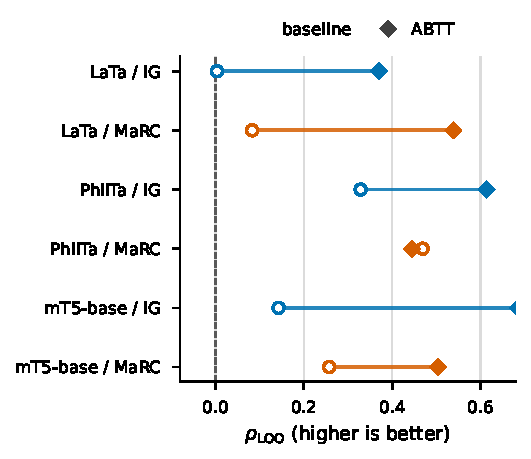
\includegraphics[width=\linewidth]{figures/fig_attribution_rho_loo_main.pdf}
\caption{Leave-one-out rank correlation $\rho_{\text{LOO}}$ at the predeclared operational attribution layers, for integrated gradients (IG) and retrieval-adapted MaRC. Each line connects the baseline and ABTT variants of one model-method cell. ABTT raises $\rho_{\text{LOO}}$ in five of the six cells; the sixth, PhilTa MaRC, moves from 0.469 to 0.445, a tie within two standard errors (Table~\ref{tab:attribution_metrics_main}). Secondary metrics: Table~\ref{tab:attribution_metrics_secondary}.}
\label{fig:attribution_rho_loo_main}
\end{figure}


% generated table
% source run: ig_examples_200pos_v1
% Selection and wording follow the part B memo behind issue #120; the numbers come from the
% run stamped above (issue #187 re-sample). Regenerate from that summary rather than
% editing the numbers here.
\begin{table*}[t]
\centering
\small
\setlength{\tabcolsep}{5pt}
\begin{tabular}{llrrrrrrrrrr}
\toprule
& & \multicolumn{2}{c}{$\tau_{\text{LOO}}$} & \multicolumn{2}{c}{InsAUC gap} & \multicolumn{2}{c}{Suff@25\%} & \multicolumn{2}{c}{Comp@25\%} & \multicolumn{2}{c}{MinFrac@0.80} \\
\cmidrule(lr){3-4}\cmidrule(lr){5-6}\cmidrule(lr){7-8}\cmidrule(lr){9-10}\cmidrule(lr){11-12}
Model & Method & base & ABTT & base & ABTT & base & ABTT & base & ABTT & base & ABTT \\
\midrule
LaTa & IG & 0.007 & \textbf{0.262} & \textbf{0.265} & 0.060 & \textbf{0.990} & 0.804 & \textbf{1.242} & 0.177 & \textbf{0.111} & 0.272 \\
 & MaRC & 0.068 & \textbf{0.400} & 0.069 & \textbf{0.137} & 0.731 & \textbf{0.917} & \textbf{0.781} & 0.280 & 0.184 & \textbf{0.177} \\
\addlinespace[2pt]
PhilTa & IG & 0.234 & \textbf{0.462} & 0.003 & \textbf{0.242} & 0.814 & \textbf{0.971} & 0.113 & \textbf{0.522} & 0.240 & \textbf{0.136} \\
 & MaRC & \textbf{0.334} & 0.318 & 0.061 & \textbf{0.190} & \textbf{0.888} & 0.878 & 0.093 & \textbf{0.363} & \textbf{0.149} & 0.259 \\
\addlinespace[2pt]
mT5-base & IG & 0.101 & \textbf{0.515} & -0.024 & \textbf{0.402} & 0.933 & \textbf{1.126} & 0.012 & \textbf{0.642} & \textbf{0.086} & 0.178 \\
 & MaRC & 0.181 & \textbf{0.359} & 0.002 & \textbf{0.329} & 0.960 & \textbf{1.013} & 0.014 & \textbf{0.582} & \textbf{0.031} & 0.246 \\
\bottomrule
\end{tabular}
\caption{Secondary attribution metrics, on the same pairs, the same layers and the same erasure operator as Table~\ref{tab:attribution_metrics_main}. Boldface marks the better variant within a pair; higher is better everywhere except MinFrac. None of these columns is in the main table, and each is out for its own reason. Kendall $\tau_b$ agrees with $\rho_{\text{LOO}}$ in 5/6 cells, but it is the tie-corrected twin of the same statistic rather than a second witness. Chance-corrected insertion faithfulness favours ABTT in 5/6 cells, and we do not report it in the main table because in one of the twelve cells, a baseline cell, the real attribution does not beat a permutation of its own scores, so the measurement does not meet the validity bar we set for a headline column. The threshold-based ERASER metrics are reported for completeness: their baseline-versus-ABTT verdict depends on the threshold and on the erasure operator, which is why the main table uses threshold-free, chance-corrected metrics instead. The InsAUC columns average 195 to 199 ABTT pairs against the baseline's 199 to 200, for the same small-denominator reason. Full threshold sweeps are in Tables~\ref{tab:attribution_sweep_main_methods} and~\ref{tab:attribution_sweep_supplemental_methods}.}
\label{tab:attribution_metrics_secondary}
\end{table*}


% generated table
\begin{table*}[t]
\centering
\scriptsize
\setlength{\tabcolsep}{2pt}
\resizebox{\textwidth}{!}{%
\begin{tabular}{llrrrrrrrrrrrrrrrrrrrrrr}
\toprule
Model & Method & \multicolumn{2}{c}{$\rho_{\text{LOO}}$~$\uparrow$} & \multicolumn{2}{c}{Suff@10\%~$\uparrow$} & \multicolumn{2}{c}{Suff@25\%~$\uparrow$} & \multicolumn{2}{c}{Suff@50\%~$\uparrow$} & \multicolumn{2}{c}{Comp@10\%~$\uparrow$} & \multicolumn{2}{c}{Comp@25\%~$\uparrow$} & \multicolumn{2}{c}{Comp@50\%~$\uparrow$} & \multicolumn{2}{c}{MinFrac@0.70~$\downarrow$} & \multicolumn{2}{c}{MinFrac@0.80~$\downarrow$} & \multicolumn{2}{c}{MinFrac@0.90~$\downarrow$} & \multicolumn{2}{c}{MinFrac@0.95~$\downarrow$} \\
\cmidrule(lr){3-4} \cmidrule(lr){5-6} \cmidrule(lr){7-8} \cmidrule(lr){9-10} \cmidrule(lr){11-12} \cmidrule(lr){13-14} \cmidrule(lr){15-16} \cmidrule(lr){17-18} \cmidrule(lr){19-20} \cmidrule(lr){21-22} \cmidrule(lr){23-24}
 &  & base & abtt & base & abtt & base & abtt & base & abtt & base & abtt & base & abtt & base & abtt & base & abtt & base & abtt & base & abtt & base & abtt \\
\midrule
LaTa & IG & 0.003 & 0.370 & 0.949 & 0.556 & 0.990 & 0.804 & 1.014 & 0.969 & 1.144 & 0.069 & 1.242 & 0.177 & 1.203 & 0.354 & 0.082 & 0.196 & 0.111 & 0.272 & 0.159 & 0.388 & 0.197 & 0.475 \\
 & MaRC & 0.083 & 0.538 & 0.696 & 0.797 & 0.731 & 0.917 & 0.807 & 1.004 & 0.487 & 0.112 & 0.781 & 0.280 & 0.889 & 0.556 & 0.139 & 0.101 & 0.184 & 0.177 & 0.270 & 0.328 & 0.317 & 0.430 \\
\midrule
PhilTa & IG & 0.329 & 0.614 & 0.637 & 0.844 & 0.814 & 0.971 & 0.937 & 1.038 & 0.042 & 0.288 & 0.113 & 0.522 & 0.231 & 0.746 & 0.156 & 0.084 & 0.240 & 0.136 & 0.411 & 0.221 & 0.548 & 0.290 \\
 & MaRC & 0.469 & 0.445 & 0.786 & 0.691 & 0.888 & 0.878 & 0.971 & 1.001 & 0.032 & 0.169 & 0.093 & 0.363 & 0.263 & 0.625 & 0.076 & 0.199 & 0.149 & 0.259 & 0.299 & 0.350 & 0.435 & 0.406 \\
\midrule
mT5-base & IG & 0.143 & 0.686 & 0.839 & 0.903 & 0.933 & 1.126 & 0.976 & 1.210 & 0.004 & 0.312 & 0.012 & 0.642 & 0.038 & 1.005 & 0.045 & 0.126 & 0.086 & 0.178 & 0.184 & 0.252 & 0.323 & 0.304 \\
 & MaRC & 0.257 & 0.504 & 0.918 & 0.791 & 0.960 & 1.013 & 0.989 & 1.121 & 0.004 & 0.274 & 0.014 & 0.582 & 0.042 & 0.902 & 0.016 & 0.175 & 0.031 & 0.246 & 0.085 & 0.347 & 0.199 & 0.412 \\
\bottomrule
\end{tabular}%
}
\caption{Appendix attribution sweep for the two paper-facing attribution views, \textsc{IG} and retrieval-adapted \textsc{MaRC}, across the three main-paper models. Direction arrows are printed in the column headers. Sufficiency and Comprehensiveness are ratio metrics at $\{10\%, 25\%, 50\%\}$; MinFrac is the minimum retained query-token fraction needed to recover $\tau \in \{0.70, 0.80, 0.90, 0.95\}$ of the full cosine (lower is better). Ratio metrics require $|S_v(q_{\text{full}}, c)| \ge 0.05$; $\rho_{\text{LOO}}$ excludes $|\Delta| < 10^{-6}$. The completeness report contains no missing metric cells.}
\label{tab:attribution_sweep_main_methods}
\end{table*}

% generated table
\begin{table*}[t]
\centering
\scriptsize
\setlength{\tabcolsep}{2pt}
\resizebox{\textwidth}{!}{%
\begin{tabular}{llrrrrrrrrrrrrrrrrrrrrrr}
\toprule
Model & Method & \multicolumn{2}{c}{$\rho_{\text{LOO}}$~$\uparrow$} & \multicolumn{2}{c}{Suff@10\%~$\uparrow$} & \multicolumn{2}{c}{Suff@25\%~$\uparrow$} & \multicolumn{2}{c}{Suff@50\%~$\uparrow$} & \multicolumn{2}{c}{Comp@10\%~$\uparrow$} & \multicolumn{2}{c}{Comp@25\%~$\uparrow$} & \multicolumn{2}{c}{Comp@50\%~$\uparrow$} & \multicolumn{2}{c}{MinFrac@0.70~$\downarrow$} & \multicolumn{2}{c}{MinFrac@0.80~$\downarrow$} & \multicolumn{2}{c}{MinFrac@0.90~$\downarrow$} & \multicolumn{2}{c}{MinFrac@0.95~$\downarrow$} \\
\cmidrule(lr){3-4} \cmidrule(lr){5-6} \cmidrule(lr){7-8} \cmidrule(lr){9-10} \cmidrule(lr){11-12} \cmidrule(lr){13-14} \cmidrule(lr){15-16} \cmidrule(lr){17-18} \cmidrule(lr){19-20} \cmidrule(lr){21-22} \cmidrule(lr){23-24}
 &  & base & abtt & base & abtt & base & abtt & base & abtt & base & abtt & base & abtt & base & abtt & base & abtt & base & abtt & base & abtt & base & abtt \\
\midrule
LaTa & BERTScore & 0.282 & 0.496 & -0.019 & 0.565 & -0.032 & 0.788 & 0.016 & 0.960 & 0.292 & 0.074 & 0.298 & 0.192 & 0.282 & 0.426 & 0.377 & 0.210 & 0.403 & 0.297 & 0.436 & 0.433 & 0.467 & 0.517 \\
 & OT & 0.031 & 0.382 & 0.929 & 0.581 & 0.961 & 0.820 & 0.979 & 0.974 & 0.872 & 0.071 & 0.882 & 0.179 & 0.827 & 0.361 & 0.087 & 0.184 & 0.115 & 0.258 & 0.160 & 0.376 & 0.197 & 0.464 \\
 & Att-weighted & -0.014 & 0.001 & -0.185 & 0.265 & -0.216 & 0.459 & 0.341 & 0.709 & 0.015 & 0.046 & 0.022 & 0.135 & 0.182 & 0.255 & 0.334 & 0.476 & 0.347 & 0.584 & 0.377 & 0.705 & 0.408 & 0.787 \\
 & Att-standalone & 0.144 & 0.575 & 0.788 & 0.721 & 0.910 & 0.905 & 0.962 & 1.010 & 0.737 & 0.108 & 0.954 & 0.275 & 1.074 & 0.553 & 0.116 & 0.132 & 0.172 & 0.209 & 0.273 & 0.341 & 0.322 & 0.436 \\
 & DLA & 0.075 & 0.601 & 0.973 & 0.704 & 1.009 & 0.893 & 1.035 & 0.989 & 1.200 & 0.123 & 1.250 & 0.292 & 1.251 & 0.555 & 0.086 & 0.128 & 0.118 & 0.208 & 0.154 & 0.353 & 0.192 & 0.452 \\
 & \textit{random} & 0.004 & -0.002 & 0.265 & 0.547 & 0.519 & 0.736 & 0.819 & 0.871 & 0.026 & 0.021 & 0.030 & 0.053 & 0.177 & 0.136 & 0.183 & 0.220 & 0.219 & 0.330 & 0.288 & 0.514 & 0.338 & 0.659 \\
 & \textit{inverse} & -0.003 & -0.370 & -0.202 & 0.276 & -0.179 & 0.436 & -0.205 & 0.653 & -0.007 & -0.017 & -0.013 & -0.022 & -0.015 & 0.035 & 0.615 & 0.513 & 0.706 & 0.645 & 0.811 & 0.797 & 0.847 & 0.883 \\
\midrule
PhilTa & BERTScore & 0.561 & 0.646 & 0.695 & 0.841 & 0.874 & 1.016 & 0.984 & 1.105 & 0.047 & 0.231 & 0.113 & 0.442 & 0.253 & 0.686 & 0.130 & 0.122 & 0.199 & 0.178 & 0.311 & 0.254 & 0.393 & 0.310 \\
 & OT & 0.340 & 0.616 & 0.641 & 0.846 & 0.818 & 0.971 & 0.940 & 1.040 & 0.043 & 0.289 & 0.114 & 0.523 & 0.233 & 0.749 & 0.152 & 0.084 & 0.237 & 0.136 & 0.401 & 0.221 & 0.541 & 0.289 \\
 & Att-weighted & 0.111 & 0.041 & 0.589 & 0.355 & 0.807 & 0.592 & 0.923 & 0.775 & 0.013 & 0.050 & 0.051 & 0.156 & 0.145 & 0.311 & 0.187 & 0.376 & 0.268 & 0.485 & 0.415 & 0.630 & 0.550 & 0.723 \\
 & Att-standalone & 0.287 & 0.217 & 0.666 & 0.486 & 0.822 & 0.705 & 0.937 & 0.888 & 0.022 & 0.095 & 0.073 & 0.240 & 0.228 & 0.458 & 0.148 & 0.270 & 0.240 & 0.358 & 0.405 & 0.479 & 0.533 & 0.560 \\
 & DLA & 0.531 & 0.599 & 0.729 & 0.872 & 0.862 & 0.970 & 0.959 & 1.006 & 0.068 & 0.311 & 0.159 & 0.567 & 0.337 & 0.776 & 0.102 & 0.069 & 0.182 & 0.115 & 0.345 & 0.205 & 0.486 & 0.285 \\
 & \textit{random} & -0.004 & -0.002 & 0.650 & 0.400 & 0.815 & 0.603 & 0.922 & 0.792 & 0.011 & 0.034 & 0.031 & 0.093 & 0.084 & 0.220 & 0.150 & 0.351 & 0.242 & 0.478 & 0.412 & 0.642 & 0.576 & 0.751 \\
 & \textit{inverse} & -0.329 & -0.614 & 0.514 & 0.046 & 0.636 & 0.109 & 0.774 & 0.255 & 0.002 & -0.030 & 0.015 & -0.049 & 0.065 & -0.038 & 0.325 & 0.859 & 0.516 & 0.909 & 0.730 & 0.951 & 0.837 & 0.970 \\
\midrule
mT5-base & BERTScore & 0.351 & 0.569 & 0.906 & 0.777 & 0.968 & 1.059 & 0.991 & 1.159 & 0.004 & 0.227 & 0.012 & 0.486 & 0.036 & 0.790 & 0.030 & 0.178 & 0.051 & 0.244 & 0.104 & 0.315 & 0.187 & 0.356 \\
 & OT & 0.151 & 0.678 & 0.840 & 0.908 & 0.933 & 1.127 & 0.976 & 1.205 & 0.004 & 0.313 & 0.012 & 0.641 & 0.039 & 0.996 & 0.045 & 0.127 & 0.086 & 0.178 & 0.183 & 0.252 & 0.321 & 0.305 \\
 & Att-weighted & 0.242 & 0.564 & 0.937 & 0.962 & 0.974 & 1.067 & 0.990 & 1.075 & 0.004 & 0.319 & 0.011 & 0.589 & 0.035 & 0.845 & 0.015 & 0.085 & 0.028 & 0.137 & 0.068 & 0.228 & 0.148 & 0.292 \\
 & Att-standalone & 0.145 & 0.268 & 0.886 & 0.616 & 0.960 & 0.760 & 0.986 & 0.857 & 0.004 & 0.221 & 0.011 & 0.412 & 0.035 & 0.587 & 0.032 & 0.270 & 0.060 & 0.374 & 0.124 & 0.499 & 0.220 & 0.586 \\
 & DLA & 0.237 & 0.552 & 0.901 & 0.934 & 0.950 & 1.051 & 0.979 & 1.032 & 0.004 & 0.341 & 0.014 & 0.622 & 0.046 & 0.825 & 0.024 & 0.083 & 0.045 & 0.133 & 0.110 & 0.231 & 0.245 & 0.312 \\
 & \textit{random} & 0.002 & 0.002 & 0.917 & 0.350 & 0.968 & 0.534 & 0.989 & 0.741 & 0.001 & 0.048 & 0.004 & 0.119 & 0.011 & 0.268 & 0.028 & 0.401 & 0.046 & 0.537 & 0.095 & 0.697 & 0.175 & 0.785 \\
 & \textit{inverse} & -0.143 & -0.686 & 0.687 & -0.201 & 0.884 & -0.186 & 0.962 & 0.002 & 0.002 & -0.092 & 0.007 & -0.168 & 0.025 & -0.210 & 0.114 & 0.869 & 0.158 & 0.912 & 0.260 & 0.953 & 0.408 & 0.974 \\
\bottomrule
\end{tabular}%
}
\caption{Supplemental attribution sweep for additional methods and sanity baselines. \textit{random} and \textit{inverse} are diagnostic baselines, not paper-facing attribution methods. Direction arrows are printed in the column headers. Sufficiency and Comprehensiveness are ratio metrics at $\{10\%, 25\%, 50\%\}$; MinFrac is the minimum retained query-token fraction needed to recover $\tau \in \{0.70, 0.80, 0.90, 0.95\}$ of the full cosine (lower is better). Ratio metrics require $|S_v(q_{\text{full}}, c)| \ge 0.05$; $\rho_{\text{LOO}}$ excludes $|\Delta| < 10^{-6}$. The completeness report contains no missing metric cells.}
\label{tab:attribution_sweep_supplemental_methods}
\end{table*}


\section{Qualitative Attribution Examples}
\label{app:qual_attribution}

This appendix keeps the example-level views for one PhilTa retrieval pair. Figure~\ref{fig:pairmatrix} gives the integrated-gradient pair matrix before and after ABTT. The attention map in Figure~\ref{fig:attention} is context only, since ABTT is applied after encoding. The retrieval-adapted MaRC masks in Figure~\ref{fig:retrieval_mark} show the learned-mask view for the same pair.

\begin{figure*}[!t]
\centering
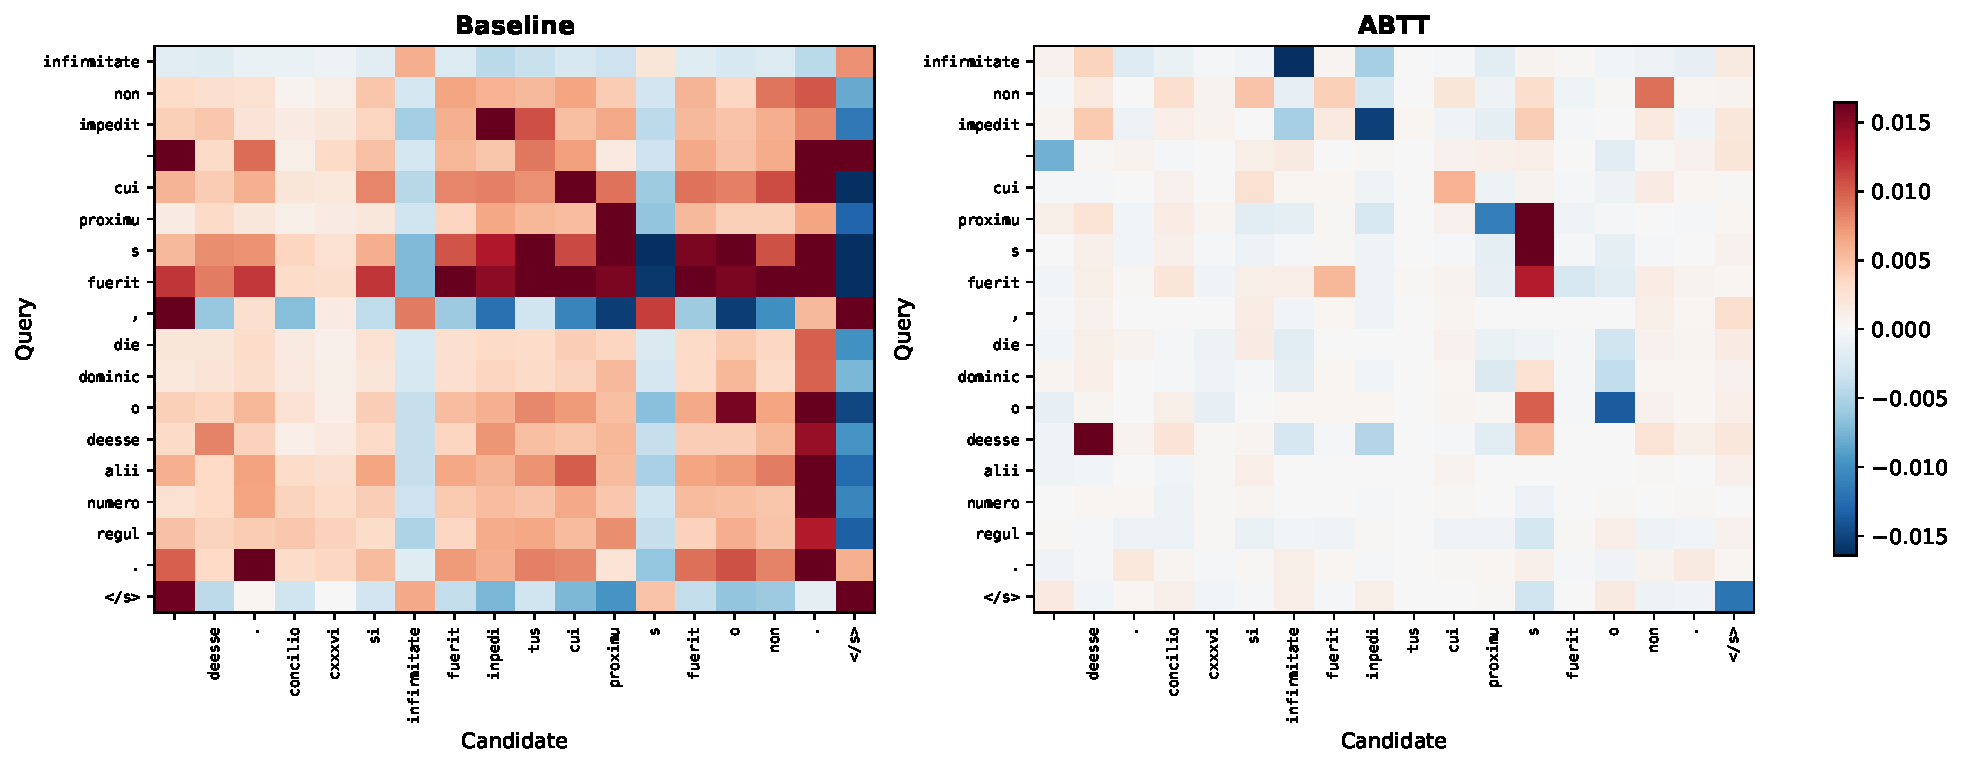
\includegraphics[width=0.94\textwidth]{fig_pair_matrix_philta.pdf}
\caption{Derived pairwise heatmap for one PhilTa retrieval case. The left panel shows the baseline representation and the right panel shows the same example after ABTT. Both axes use original decoded tokens. Cell values combine token-token cosine similarity with single-sequence integrated-gradient scores.}
\label{fig:pairmatrix}
\end{figure*}

\begin{figure*}[!t]
\centering
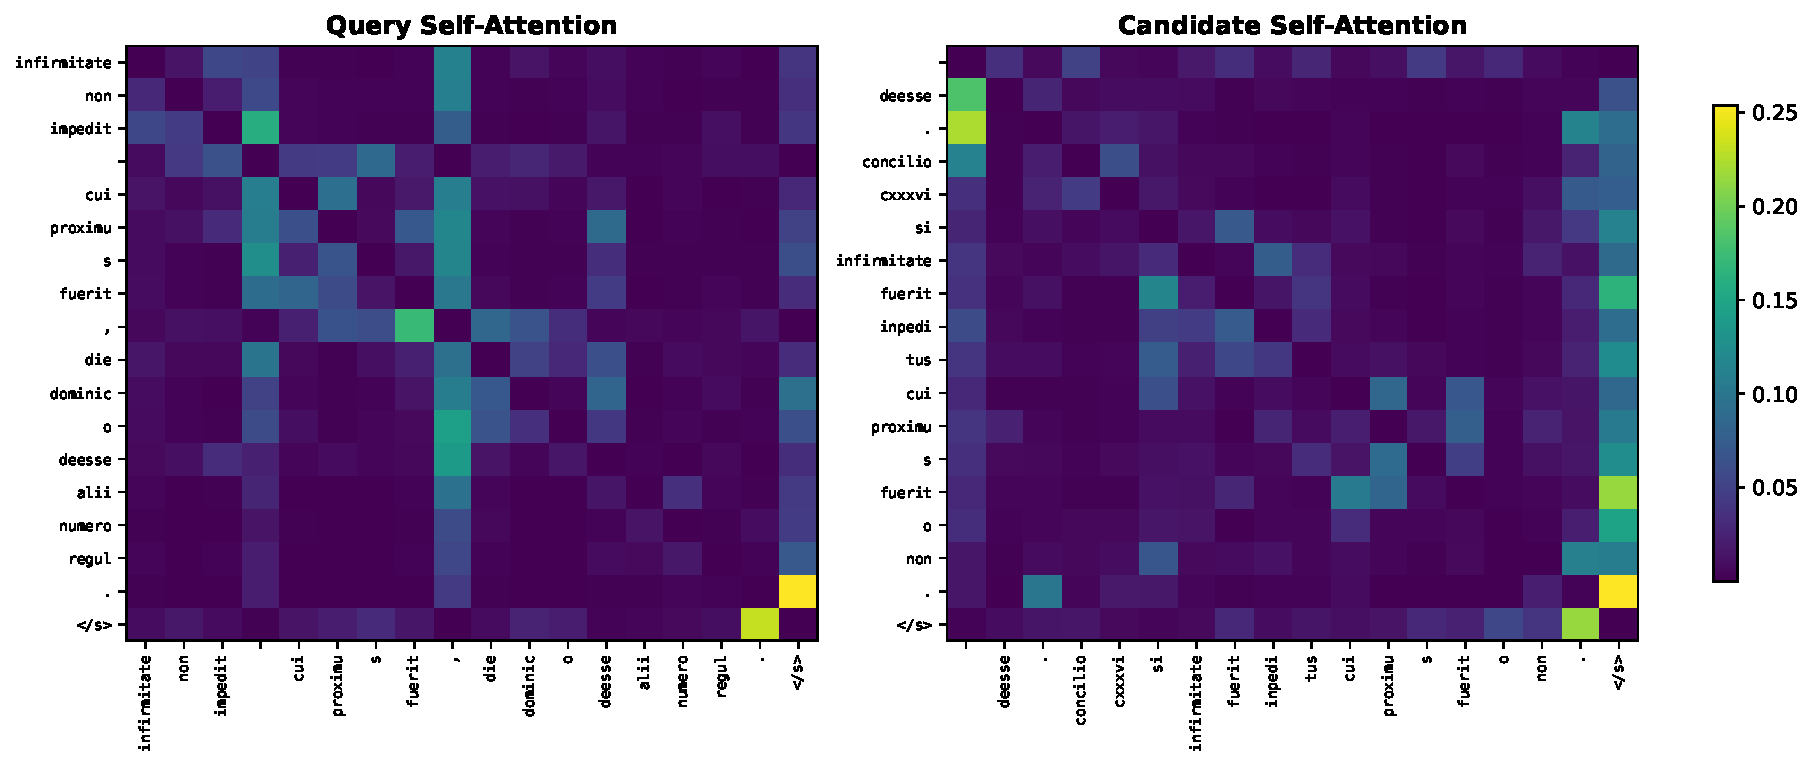
\includegraphics[width=0.94\textwidth]{fig_attention_philta.pdf}
\caption{Companion self-attention maps for the same PhilTa example as Figure~\ref{fig:pairmatrix}. ABTT is applied after encoding, so attention is included only as supporting context.}
\label{fig:attention}
\end{figure*}

\begin{figure*}[!t]
\centering
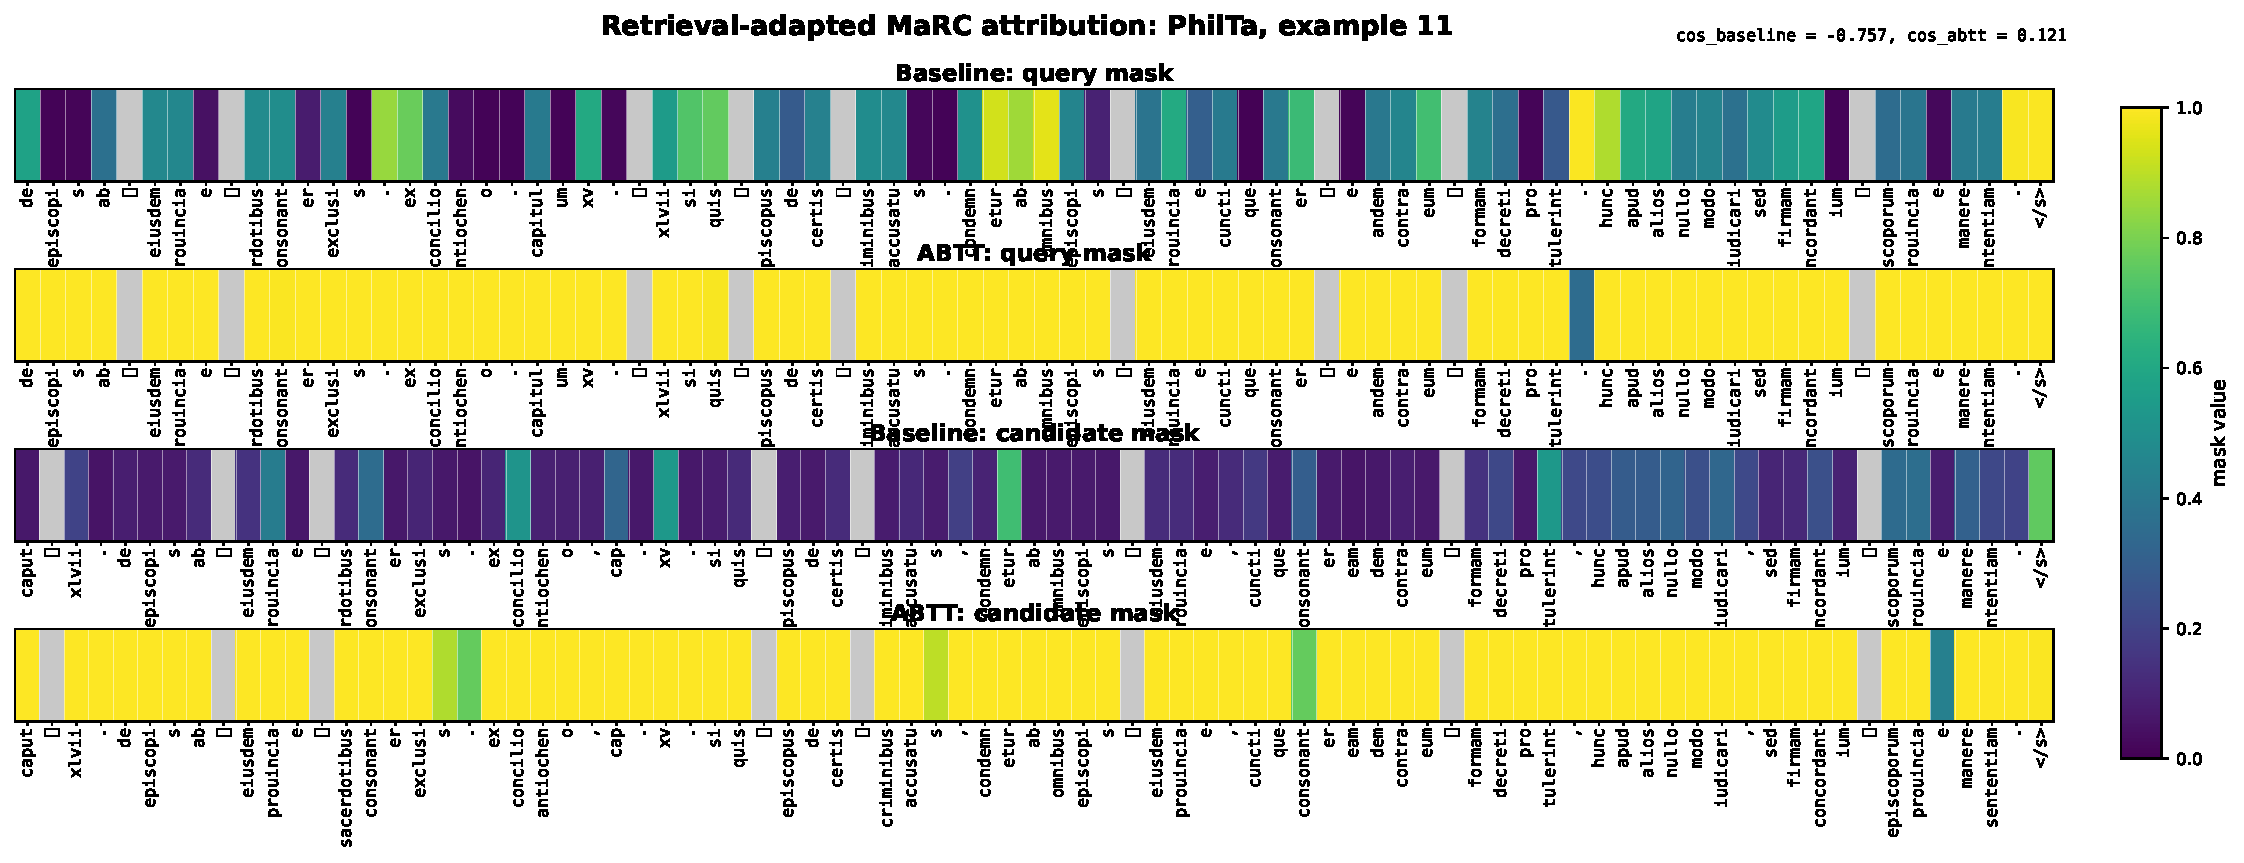
\includegraphics[width=0.94\textwidth]{fig_retrieval_mark_pair_philta.pdf}
\caption{Retrieval-adapted MaRC masks for the same PhilTa pair as Figure~\ref{fig:pairmatrix}. Top row: mask on the query with the candidate fixed. Bottom row: mask on the candidate with the query fixed. Left column: baseline cosine target. Right column: ABTT-corrected cosine target.}
\label{fig:retrieval_mark}
\end{figure*}

\section{Cluster Geometry}
\label{app:cluster_geometry}

Figures~\ref{fig:tsne} and~\ref{fig:umap} give the t-SNE and UMAP panels for LaTa, PhilTa, and mT5-base, and Figures~\ref{fig:tsne_appendix} and~\ref{fig:umap_appendix} extend them to LaBSE, Qwen3-0.6B, and KaLM-mini. All four draw all 1,705 witnesses, color the same six largest directories, and compare baseline mean pooling with ABTT-only at $D=10$; each model sits at the layer chosen on the train split by directory accuracy at rank~1 under ABTT, the ABTT subscript of Table~\ref{tab:taskB_headline}.

\begin{figure*}[!t]
\centering
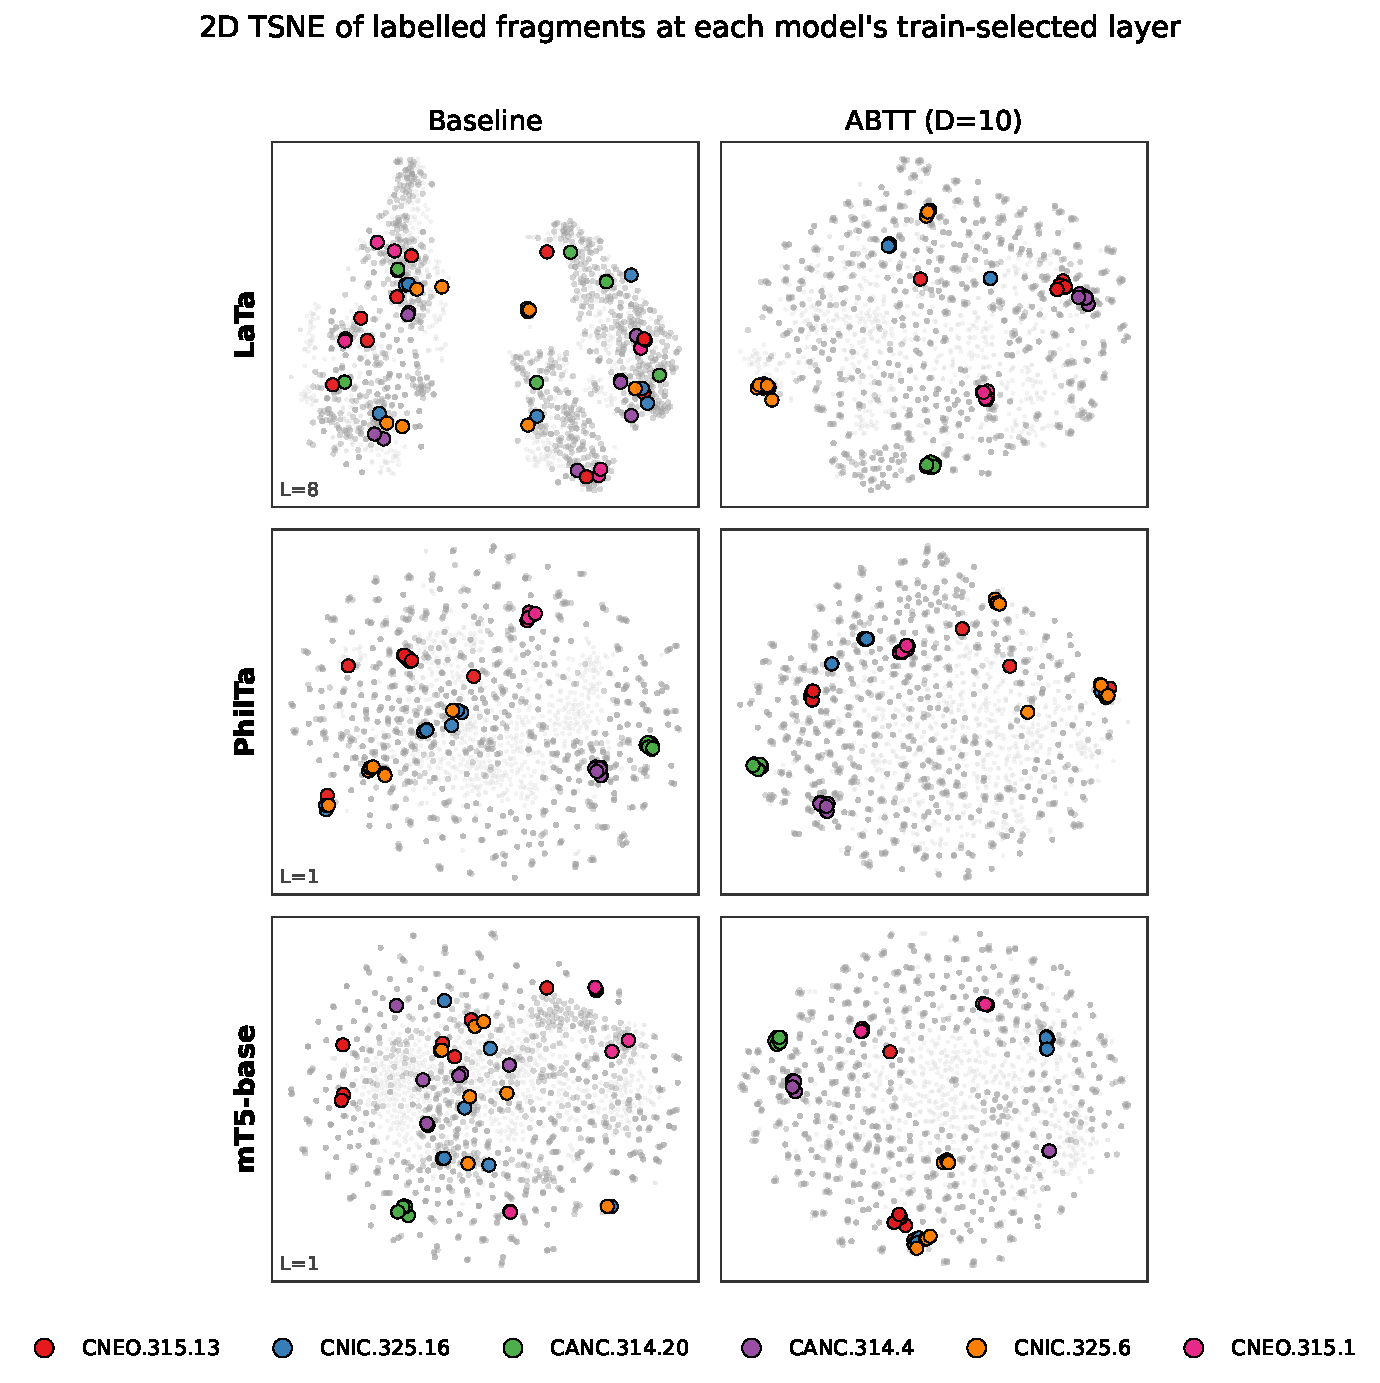
\includegraphics[width=\textwidth]{fig_tsne_main.pdf}
\caption{t-SNE projections of all 1,705 manuscript witnesses for LaTa, PhilTa, and mT5-base, each at the layer chosen on the train split: the layer with the highest training-set directory accuracy at rank~1 under ABTT, printed in each panel as L and equal to the ABTT subscript in Table~\ref{tab:taskB_headline}. Columns compare baseline mean pooling with ABTT-only using $D=10$, fit on the training embeddings. Colors mark the six largest directories; other witnesses of directories with at least two witnesses are mid gray, and singletons light gray. The silhouette scores in Section~\ref{sec:results} are computed in these two-dimensional coordinates over the 1,160 winnable witnesses, those whose directory has at least two witnesses.}
\label{fig:tsne}
\end{figure*}

\begin{figure*}[!t]
\centering
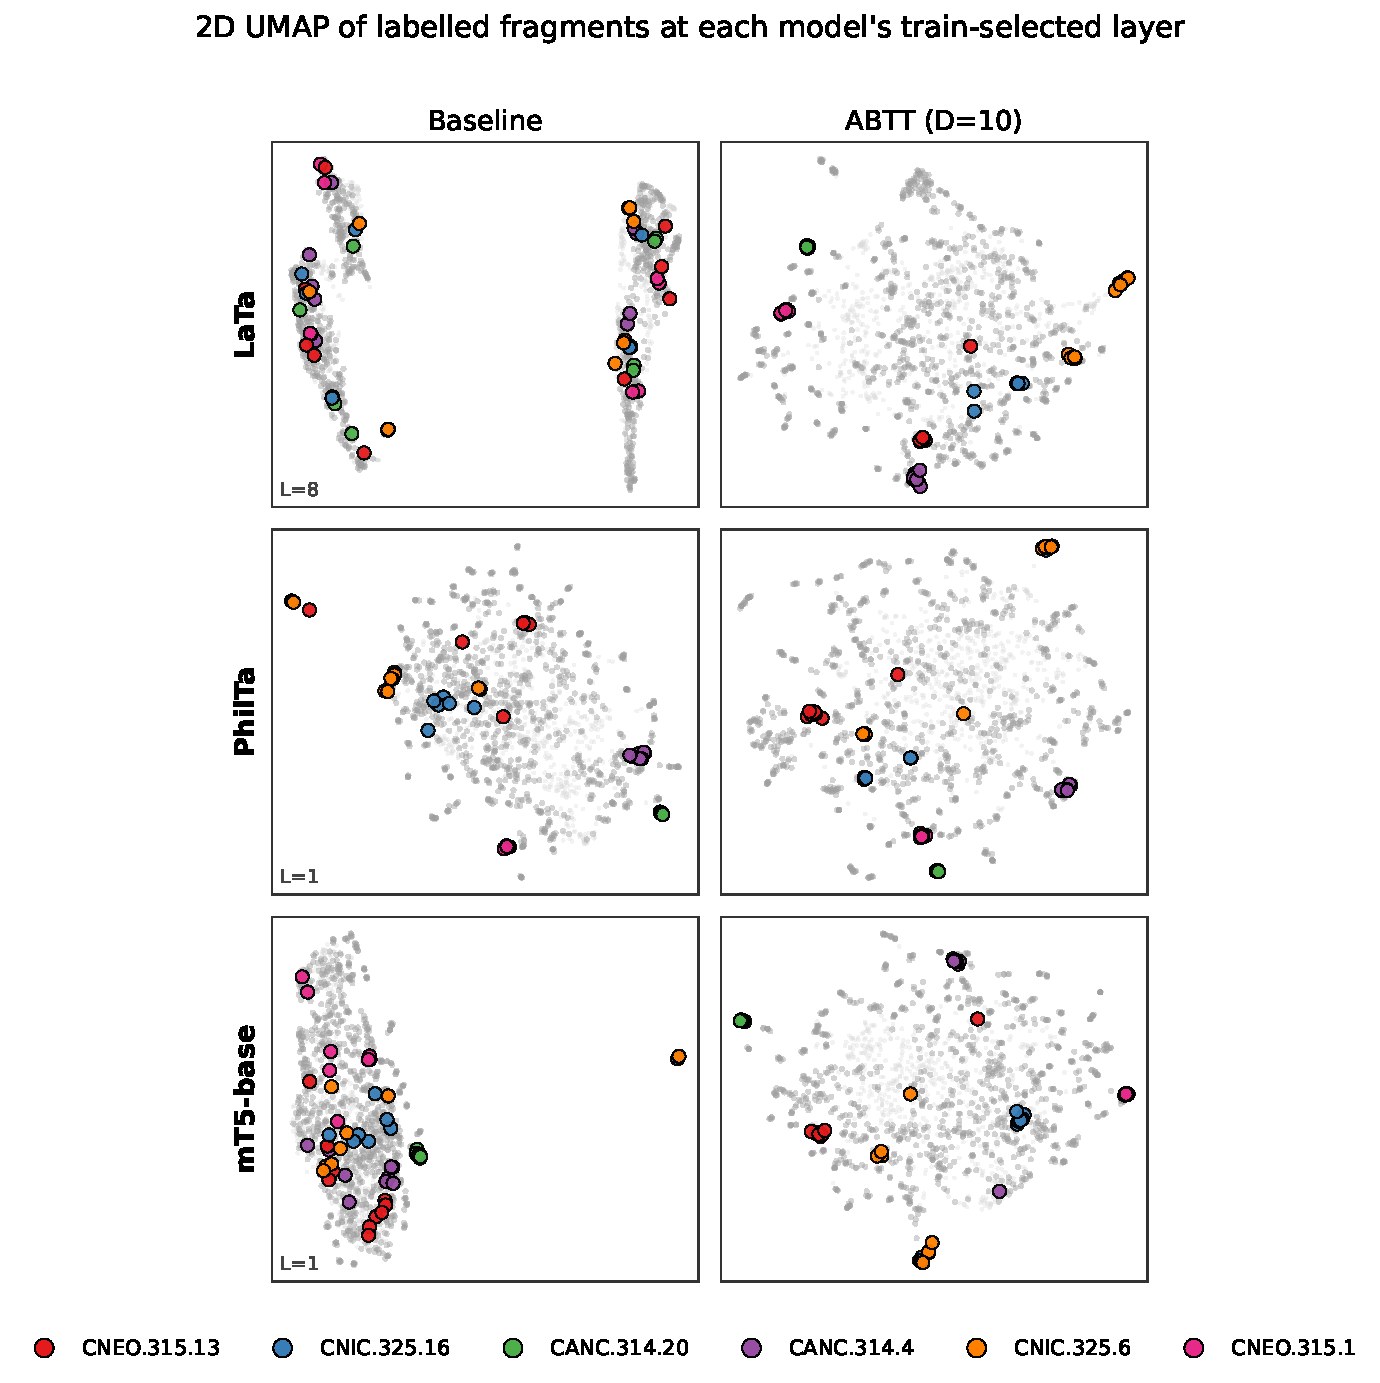
\includegraphics[width=\textwidth]{fig_umap_main.pdf}
\caption{UMAP projections with the same configuration as Figure~\ref{fig:tsne}. The same cluster-tightening pattern appears under a different projection method.}
\label{fig:umap}
\end{figure*}

\begin{figure*}[!t]
\centering
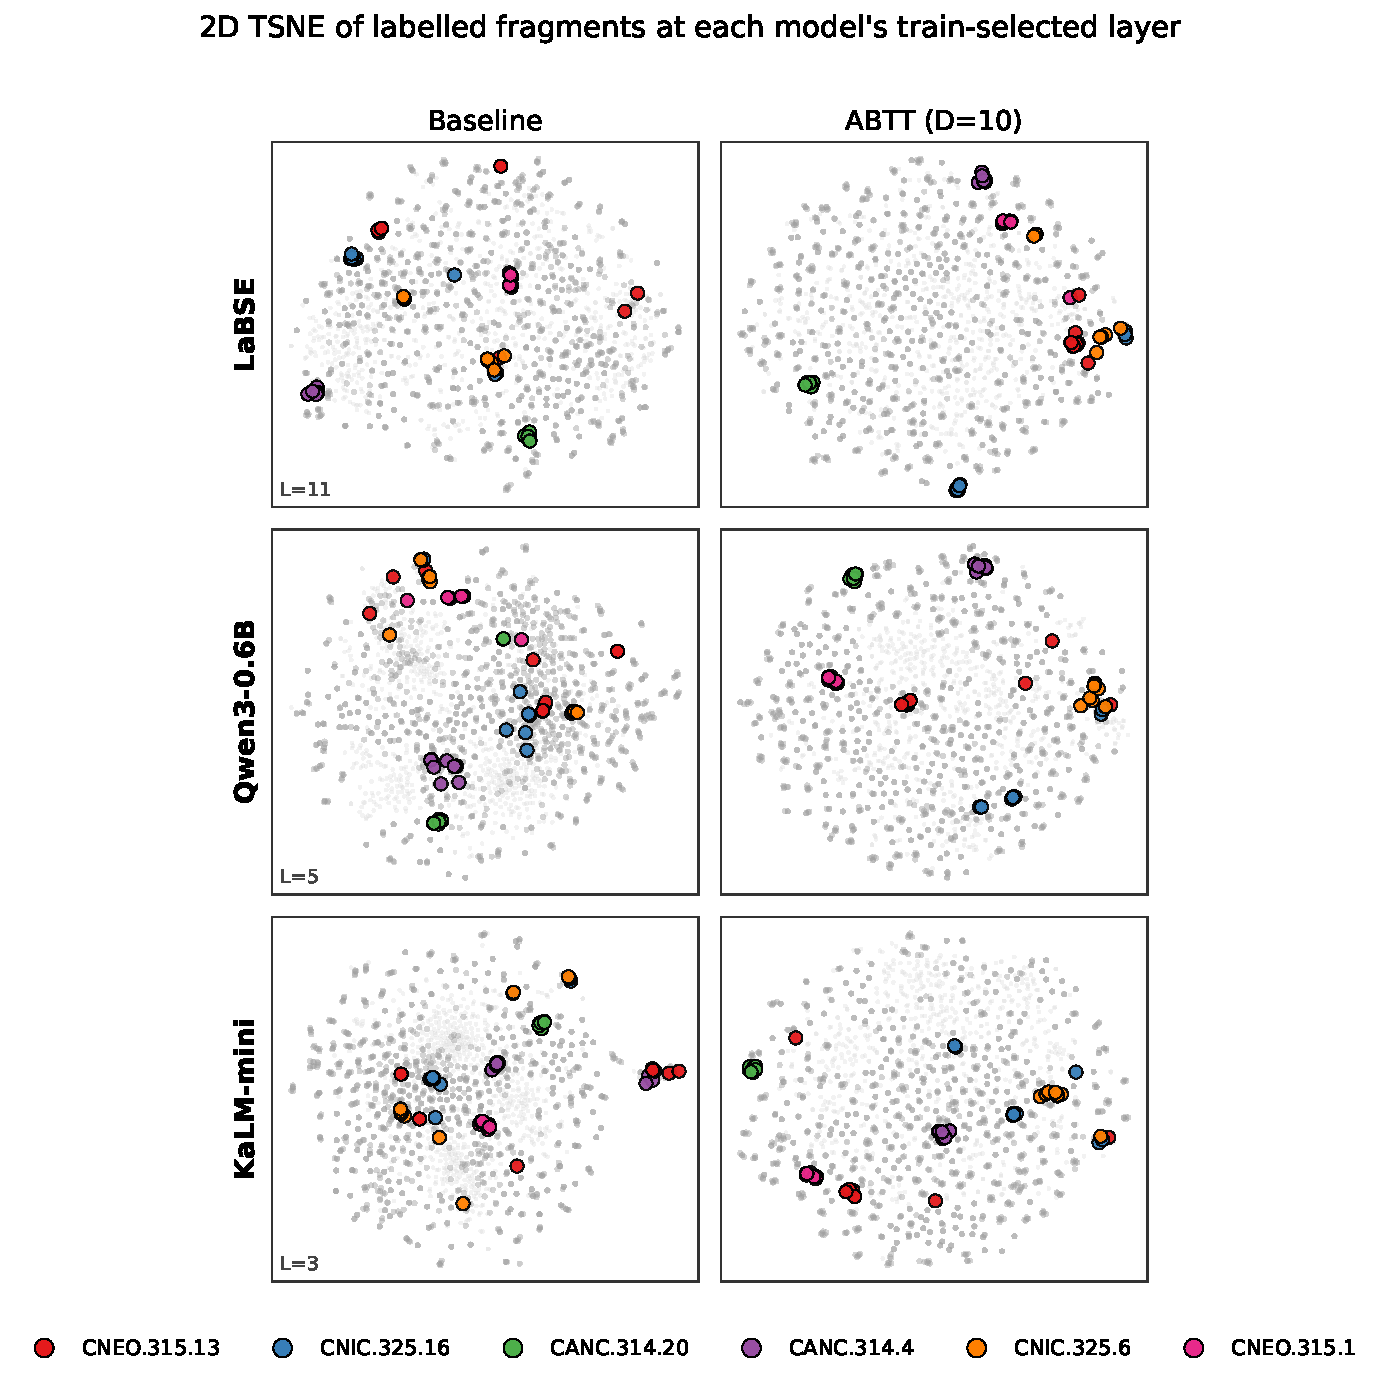
\includegraphics[width=\textwidth]{fig_tsne_appendix.pdf}
\caption{t-SNE projections of all 1,705 manuscript witnesses for LaBSE, Qwen3-0.6B, and KaLM-mini under the layer rule of Figure~\ref{fig:tsne}: the layer with the highest training-set directory accuracy at rank~1 under ABTT, printed in each panel and equal to the ABTT subscript in Table~\ref{tab:taskB_headline}. Columns compare baseline mean pooling with ABTT-only using $D=10$. Colors mark the same six largest directories as Figure~\ref{fig:tsne}.}
\label{fig:tsne_appendix}
\end{figure*}

\begin{figure*}[!t]
\centering
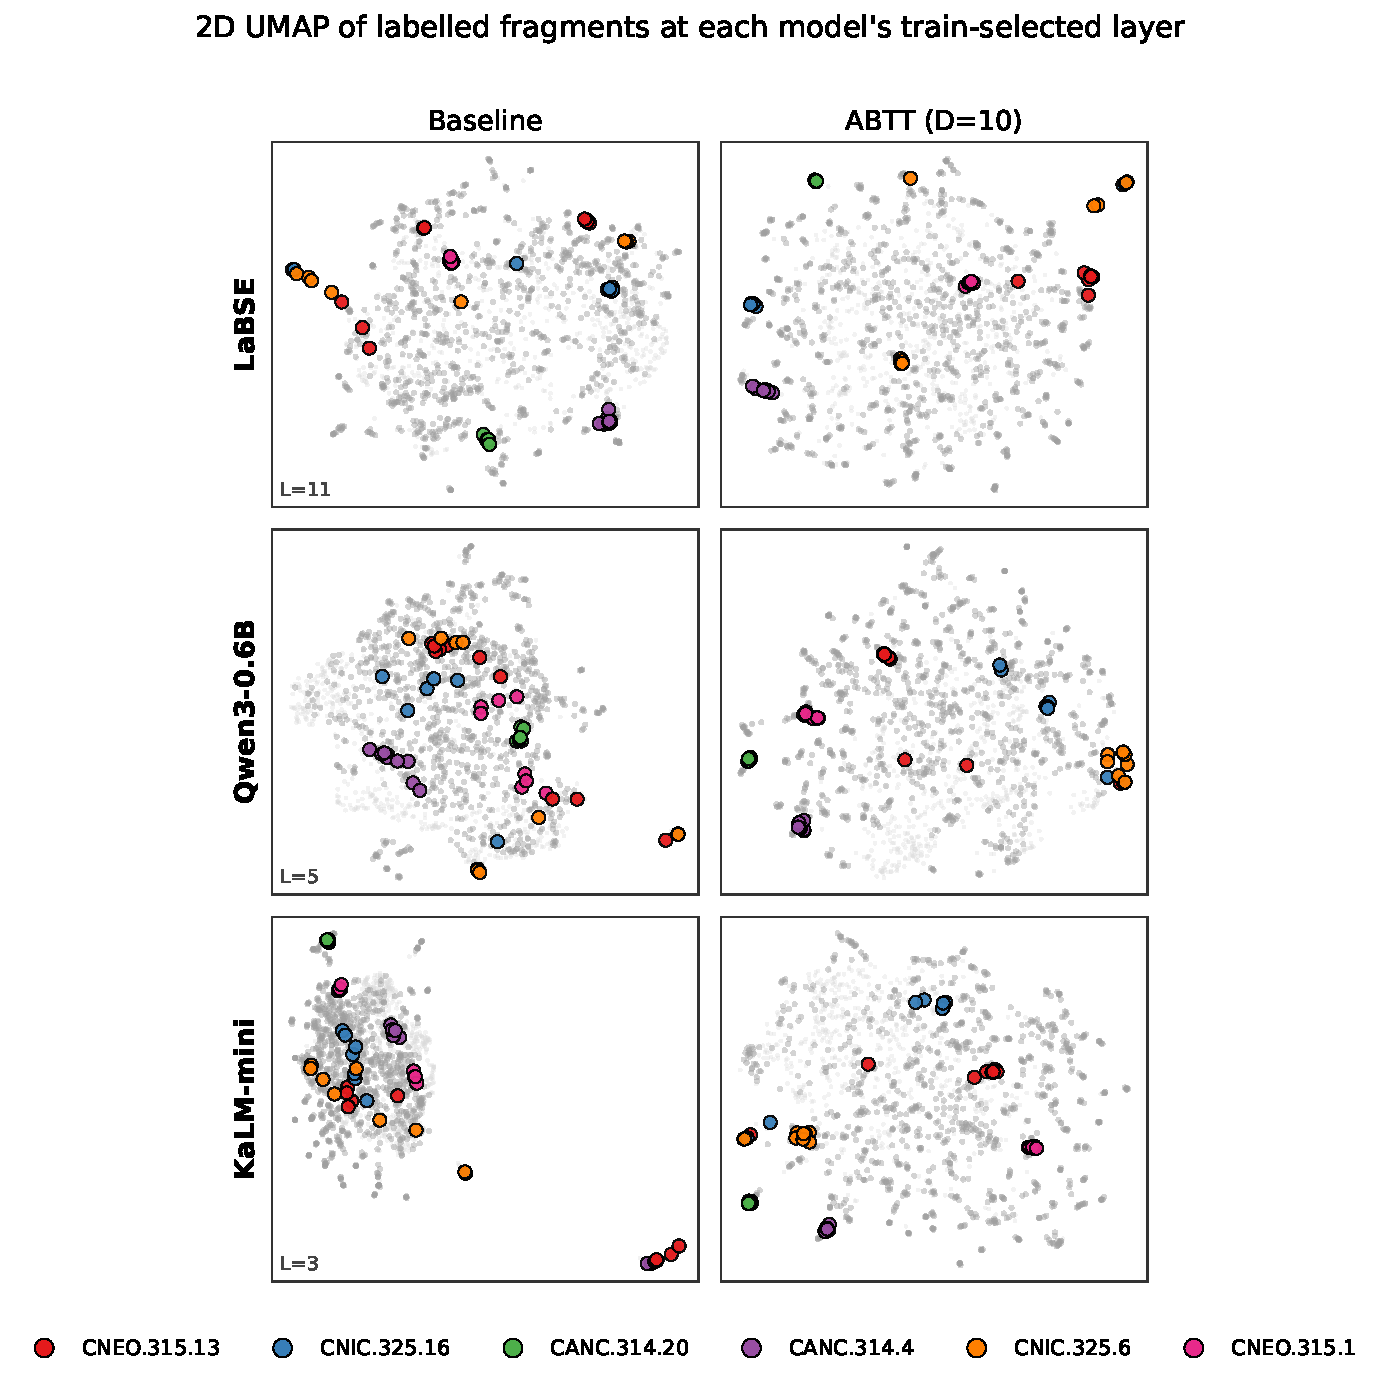
\includegraphics[width=\textwidth]{fig_umap_appendix.pdf}
\caption{UMAP projections matching Figure~\ref{fig:tsne_appendix}. The cluster-tightening pattern appears under a second projection method.}
\label{fig:umap_appendix}
\end{figure*}

\end{document}
